% !TEX root = projekt.tex
        % Tento soubor nahraďte vlastním souborem s obsahem práce.
        %=========================================================================
        % Autoři: Michal Bidlo, Bohuslav Křena, Jaroslav Dytrych, Petr Veigend a Adam Herout 2019
      
        % Pro kompilaci po částech (viz projekt.tex), nutno odkomentovat a upravit
        %\documentclass[../projekt.tex]{subfiles}
        %\begin{document}
      
        \chapter{Úvod}
      
        Mobilná robotika dnes umožňuje vytvárať autonómne systémy aj na relatívne dostupnom hardvéri. Na prvý pohľad sa môže zdať, že postaviť robota, ktorý sa pohybuje v priestore, vyhýba sa prekážkam a reaguje na okolie, je len otázkou poskladania niekoľkých komponentov. V praxi však takéto riešenie prináša množstvo problémov, akými sú napríklad nepresný odhad polohy, šum v senzoroch, obmedzený výkon zariadenia alebo samotná zložitosť prepojenia všetkých častí do jedného funkčného systému.
      
        Táto práca sa zameriava práve na tieto výzvy a ukazuje, ako je možné navrhnúť a postupne vybudovať robotické riešenie založené na ROS~2. Cieľom je vytvoriť zostavu, ktorá zvládne nielen jednoduché diaľkové ovládanie, ale aj základné autonómne správanie. Zároveň je architektúra navrhnutá tak, aby jednotlivé časti boli oddelené a dali sa samostatne upravovať alebo rozširovať.
      
        Riešenie je implementované na podvozku \emph{Wave Rover} od spoločnosti Waveshare, doplnenom o mikropočítač Raspberry Pi~5 a kameru. Zostava je rozdelená medzi samotného robota a externý počítač s Ubuntu~24.04, čo pomáha lepšie využiť dostupný výkon a jednoduchšie testovať jednotlivé časti.
      
        V priebehu práce vysvetlím, ako robot spracúva dáta zo senzorov, ako sa pohybuje aj bez presného merania kolies a ako sa dokáže vyhnúť prekážkam alebo orientovať v prostredí. Okrem toho sú predstavené aj rozšírenia, ako mapovanie prostredia (SLAM), jednoduchá navigácia, simulácia v prostredí Gazebo či sledovanie farebného objektu pomocou kamery.
      
        Práca je rozdelená do viacerých kapitol. Druhá kapitola predstavuje použitý hardvér, tretia približuje princípy ROS~2 a spôsob, akým spolu jednotlivé časti systému komunikujú. Štvrtá kapitola sa venuje samotnému návrhu a implementácii riešenia a záver obsahuje testovanie, vyhodnotenie výsledkov a diskusiu o možnostiach ďalšieho rozvoja.
      
      
      
        \chapter{Hardvérové vybavenie}
        \label{chap:hardware}
      
        Hardvér robota tvorí základ celého systému a priamo ovplyvňuje jeho možnosti aj obmedzenia. Pri mobilnej platforme nestačí navrhnúť iba softvér, dôležité je poznať aj spôsob riadenia motorov, dostupné senzory, výpočtovú jednotku a rozhrania, cez ktoré spolu jednotlivé časti komunikujú.
      
        Táto kapitola preto predstavuje komponenty použité v práci a zároveň vysvetľuje, akú úlohu majú v navrhnutom riešení. Postupne je opísaný jednodoskový počítač Raspberry Pi, podvozok Wave Rover s pohonom, doplnkové riadiace dosky, senzory a komunikačné rozhrania.
      
        \section{Raspberry Pi 5}
      
        Raspberry Pi tvorí hlavnú výpočtovú časť robota. Beží na ňom ROS~2, spracovanie senzorických dát aj väčšina riadiacej logiky. Preto je vhodné najprv stručne priblížiť jeho vlastnosti a úlohu v systéme.
      
        Raspberry Pi~5 je kompaktný jednodoskový počítač určený na vývoj a prototypovanie\footnote{Oficiálna dokumentácia Raspberry Pi: \url{https://www.raspberrypi.com/documentation/}.}. Často sa používa v projektoch z oblasti elektroniky, internetu vecí a robotiky, pretože ponúka dostatočný výkon pri malých rozmeroch a nízkej spotrebe.
      
        \begin{figure}[H] 
            \centering
            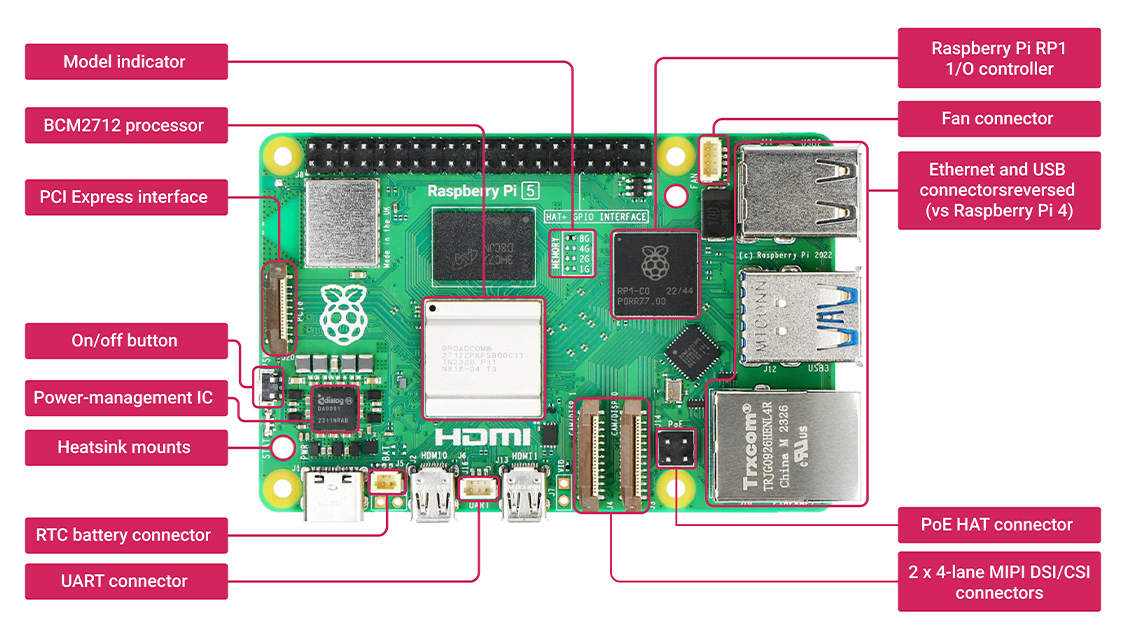
\includegraphics[width=0.7\textwidth]{obrazky/Raspberry_Pi_5_Specifications.jpg} 
            \caption{Špecifikácie Raspberry Pi~5 (prehľad platformy)}
            \label{fig:rpi5-specs}
        \end{figure}
      
        \subsection*{Architektúra}
      
        Raspberry Pi~5 je založené na architektúre ARM a využíva procesor Cortex-A76, ktorý má štyri jadrá pracujúce na frekvencii 2,4\,GHz. Vďaka tomu dokáže paralelne spracovávať viacero úloh, čo je pri robotickom systéme dôležité pri súčasnom spracovaní dát z kamery, LiDARu, IMU a riadení pohonu.
      
        Na platforme Wave Rover je Raspberry Pi pripojené cez GPIO piny. Tie je možné použiť ako vstupy na čítanie signálov alebo ako výstupy na ovládanie ďalších periférií.
      
        \section{Wave Rover}
      
        Wave Rover predstavuje mobilnú platformu\footnote{Produktová stránka Wave Rover: \url{https://www.waveshare.com/wave-rover.htm}.}, na ktorej je celé riešenie postavené. Poskytuje podvozok, kolesá, pohon a priestor na rozšírenie o ďalšie komponenty.
      
        Ide o experimentálnu platformu pre mobilnú robotiku: podvozok a kolesá sú navrhnuté tak, aby boli stabilné a odolné voči náročnejším povrchom, v základnej zostave sú senzory a aktuátory a zostáva priestor na modifikácie podľa aplikácie.
      
        \begin{figure}[H]
            \centering
            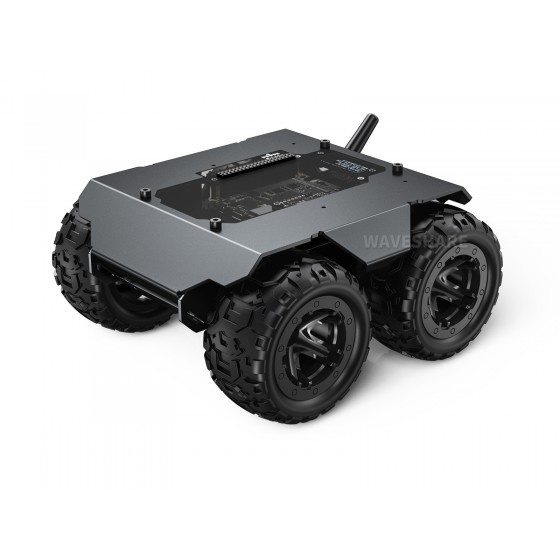
\includegraphics[width=0.4\textwidth]{obrazky/wave-rover-1.jpg}
            \caption[Wave Rover]{Platforma Wave Rover v pôvodnej zostave}
            \label{fig:wave-rover-base}
        \end{figure}
      
        \section{Motory a pohon podvozku}
      
        Pohyb robota je zabezpečený jednosmernými motormi. Keďže riadenie pohybu patrí medzi najdôležitejšie časti celej práce, najprv treba vysvetliť, ako takýto motor funguje a ako sa dá jeho rýchlosť a smer ovládať.
      
        \subsection*{Jednosmerný elektromotor}
      
        Pohon kolies zabezpečujú jednosmerné elektromotory. Ich princíp spočíva v elektrickom prúde, ktorý preteká vinutím rotora. Tým v magnetickom poli statora vzniká elektromagnetická sila a následne krútiaci moment na hriadeli. Aby sa rotor nepootočil iba jednorazovo, ale otáčal sa plynulo, treba priebežne meniť smer prúdu vo vinutí. Motor tak premieňa elektrickú energiu na mechanický pohyb.
      
        Rýchlosť otáčania motora sa riadi pomocou PWM (\emph{Pulse Width Modulation}) signálu. PWM nemení priamo veľkosť napätia, ale jeho časový priebeh. Napájanie sa rýchlo prepína medzi zapnutým a vypnutým stavom a pomer medzi týmito stavmi určuje výslednú strednú hodnotu napätia privádzaného na motor. Vďaka tomu je možné regulovať rýchlosť otáčania bez potreby analógovej regulácie napätia.
      
        Zmenu smeru otáčania zabezpečuje H-most, ktorý umožňuje prehodiť polaritu napájania motora~\cite{hyperphysics_dc_motor}.
      
        \begin{figure}[H]
            \centering
            \begin{minipage}[t]{0.48\textwidth}
                \centering
                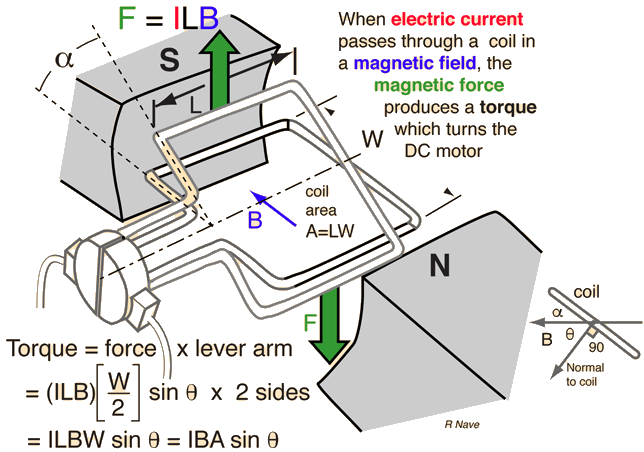
\includegraphics[width=\linewidth]{obrazky/dc.png}\\[0.35em]
                {\small Princíp kefkového jednosmerného motora}
            \end{minipage}
            \hfill
            \begin{minipage}[t]{0.48\textwidth}
                \centering
                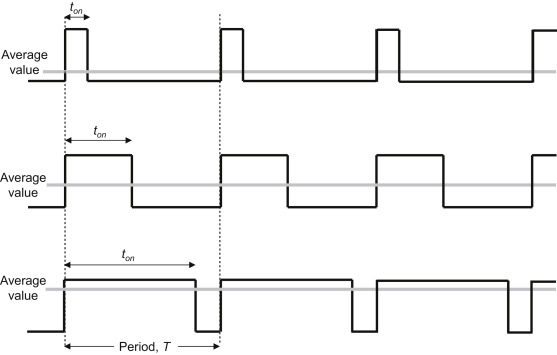
\includegraphics[width=\linewidth]{obrazky/pwm.jpg}\\[0.35em]
                {\small PWM: rovnaká perioda $T$, priemerná hodnota od $t_{\mathrm{on}}$}
            \end{minipage}
            \caption[Vľavo DC motor, vpravo PWM]{Vľavo ilustrácia princípu kefkového jednosmerného motora. Vpravo šírkovo-pulzná modulácia (PWM) --- pri rovnakej perióde $T$ závisí priemerná hodnota signálu od dĺžky impulzu $t_{\mathrm{on}}$ (striedy).}
            \label{fig:dc-motor-principle}
        \end{figure}
      
        Podvozok robota je diferenciálny. Ľavá a pravá strana pohonu sú riadené nezávisle, čo umožňuje jazdu vpred, vzad aj otáčanie na mieste. V práci sa pracuje s dvomi vetvami riadenia. Hlavná nasadená konfigurácia využíva Motor Driver HAT na Raspberry Pi, kde sa PWM signály pre H-mosty nastavujú cez čip PCA9685 na zbernici I\textsuperscript{2}C~\cite{nxp_pca9685}. Druhou vetvou je referenčná výrobná alternatíva založená na doske General Driver for Robots s mikrokontrolérom ESP32 a HTTP API od Waveshare, ktorá je opísaná v nasledujúcej časti.
      
        \section{General Driver for Robots}
      
        Doska General Driver for Robots predstavuje výrobnú alternatívu riadenia podvozku. V práci bola použitá najmä na overenie pôvodného spôsobu ovládania platformy a ako porovnanie s vlastnou implementáciou riadenia cez Motor Driver HAT.
      
        General Driver for Robots patrí k ekosystému Waveshare\footnote{Waveshare Wiki k doske General Driver for Robots: \url{https://www.waveshare.com/wiki/General_Driver_for_Robots}.}. Je založený na module ESP32-WROOM-32 a podporuje bezdrôtové rozhrania WiFi, Bluetooth a ESP-NOW. ESP32 tu funguje ako sprostredkovateľ medzi hardvérom a vyššou riadiacou logikou. Obr.~\ref{fig:general-driver-board} znázorňuje dosku s číslovaním podľa výrobcu a v tabuľke~\ref{tab:general-driver-onboard} sú uvedené vybrané položky dôležité pre nadväznosť na Raspberry Pi, LiDAR, pohon a palubnú IMU. Úplný popis označení uvádza rovnaký zdroj.
      
        Pre odhad orientácie doska využíva integrovanú deväťosovú IMU, ktorá pozostáva zo šesťosového senzora pohybu a trojosového magnetometra. Motory ovláda čip TB6612FNG, ďalšie údaje o palubných blokoch, schémach a open-source ukážkach uvádza dokumentácia výrobcu. Prepojenie s ROS~2 cez HTTP a firmvér UGV Base General je podrobnejšie rozobrané v kapitole o implementácii.
      
        \begin{figure}[H]
            \centering
            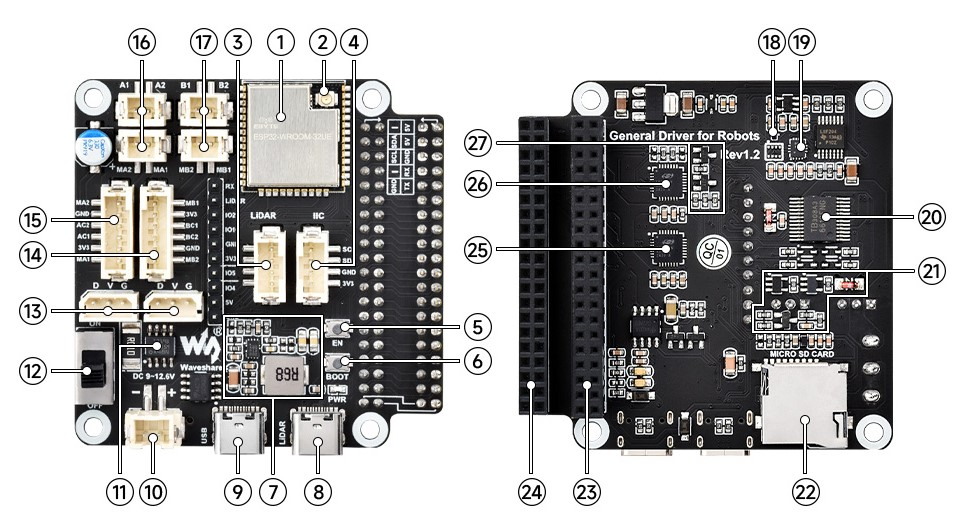
\includegraphics[width=0.6\textwidth]{obrazky/General_Driver_for_Robot02.jpg}
            \caption[General Driver for Robots]{Doska General Driver for Robots (Waveshare) s vyznačenými palubnými zdrojmi; číslovanie zodpovedá tabuľke~\ref{tab:general-driver-onboard} a dokumentácii výrobcu}
            \label{fig:general-driver-board}
        \end{figure}
      
        {\footnotesize
        \begin{table}[H]
          \centering
          \begin{tabular}{@{}r >{\raggedright\arraybackslash}p{0.32\textwidth} >{\raggedright\arraybackslash}p{0.48\textwidth}@{}}
            \toprule
            Č. & Palubný zdroj / rozhranie & Stručný význam pre robotiku \\
            \midrule
            1 & ESP32-WROOM-32 & Hlavný mikrokontrolér; nízkoúrovňové riadenie a firmvér. \\
            \midrule
            3 & Rozhranie LiDAR & Konektor pre LiDAR. \\
            \midrule
            7 & Obvod DC--DC 5\,V & Napájanie hostiteľa (Raspberry Pi) z palubného napájania. \\
            \midrule
            8--9 & Type-C (LiDAR / USB) & Dátové prepojenie LiDARu a USB/UART pre ESP32 (programovanie a sériová linka). \\
            \midrule
            10 & Napájací port XH2.54 & Vstup DC 7--13\,V pre motory a súvisiace okruhy. \\
            \midrule
            14--17 & Motor PH2.0 (6P / 2P) & Skupiny A/B: motory s enkodérom (6P) alebo bez enkodéra (2P). \\
            \midrule
            18--19 & AK09918C, QMI8658 & Palubná deväťosová IMU. \\
            \midrule
            20 & TB6612FNG & H-mostové ovládanie jednosmerných motorov. \\
            \midrule
            23--24 & 40-pinové rozšírenie & Kompatibilný konektor pre osadenie na Raspberry Pi (hostiteľ ROS~2). \\
            \midrule
            25--26 & CP2102 (LiDAR, ESP32) & USB--UART mostíky pre dátový tok LiDARu a komunikáciu s ESP32. \\
            \bottomrule
          \end{tabular}
          \caption[Výber blokov General Driver]{Výber najdôležitejších palubných blokov dosky General Driver for Robots podľa číslovania (obr.~\ref{fig:general-driver-board}).}
          \label{tab:general-driver-onboard}
        \end{table}
        }
      
        \subsubsection*{Arduino Nano ako doplnková jednotka pre IMU}
      
        Okrem Raspberry Pi a Motor Driver HAT je v realizačnej zostave použité Arduino Nano
        ako malý mikrokontrolér výhradne na čítanie IMU dát z MPU-6050 a streamovanie údajov
        po USB. Dôvodom bolo, aby senzor nezdieľal I\textsuperscript{2}C zbernicu(\ref{sec:i2c}) s motorovým HATom na strane
        RPi, čím sa zvýšila spoľahlivosť čítania a zápisu dát pri vyšších frekvenciách
        pre riadenie motorov aj spracovanie IMU.
      
        \begin{figure}[H]
            \centering
            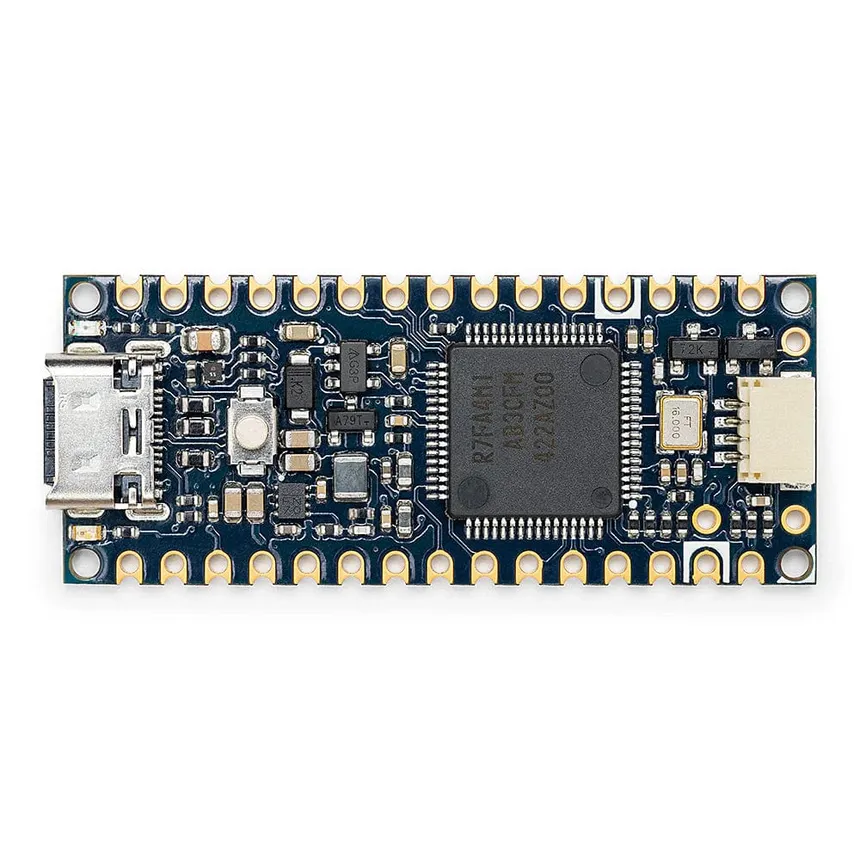
\includegraphics[width=0.4\textwidth]{obrazky/arduinonano.png}
            \caption[Arduino Nano]{Arduino Nano R4 použité v zostave ako mikrokontrolér pre MPU-6050 a USB výstup dát na Raspberry Pi}
            \label{fig:arduino-nano-imu}
        \end{figure}
      
        \section*{Inerciálna meracia jednotka (IMU)}
      
        IMU poskytuje informácie o pohybe a orientácii robota. Keďže použitý podvozok nemá enkodéry na kolesách, tieto dáta sú dôležité pri stabilizácii jazdy a odhade orientácie robota.
      
        \subsection*{Akcelerometer}
      
        V module IMU MPU-6050 sa nachádza trojosový akcelerometer, ktorý meria lineárne zrýchlenie pôsobiace v osiach senzora. MEMS akcelerometer využíva kapacitný princíp, pri ktorom sa vnútorný hmotný prvok pri zrýchlení vychyľuje. Tým sa mení kapacita štruktúry a táto zmena sa následne prevedie na elektrický signál.
      
        Okrem dynamického zrýchlenia sa v meraní prejavuje aj gravitačné zrýchlenie. Pri pomalom alebo ustálenom pohybe preto možno zo zložiek gravitácie v súradnicovej sústave senzora odhadovať náklon zariadenia voči zemi. V robotických aplikáciách sa tieto údaje využívajú napríklad pri stabilizácii pohybu alebo ako doplnková informácia pre odhad orientácie.
      
        Pri dynamickom pohybe však meranie obsahuje aj zrýchlenie spôsobené samotným pohybom podvozku, čo môže odhad náklonu skresliť. Z tohto dôvodu sa akcelerometer v praxi často kombinuje s gyroskopom alebo s metódami senzorovej fúzie~\cite{analog_devices_accel_gyro}, ktoré umožňujú získať stabilnejší odhad orientácie.
      
        \begin{figure}[H]
            \centering
            \begin{minipage}[t]{0.48\textwidth}
                \centering
                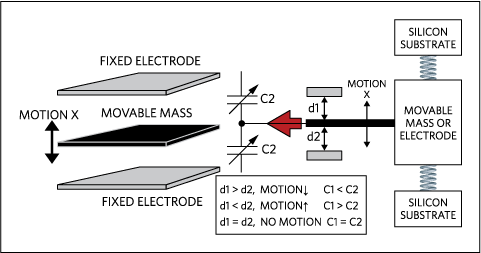
\includegraphics[width=\linewidth]{obrazky/acelerometer.png}\\[0.35em]
                {\small Ilustrácia MEMS akcelerometra}
            \end{minipage}
            \hfill
            \begin{minipage}[t]{0.48\textwidth}
                \centering
                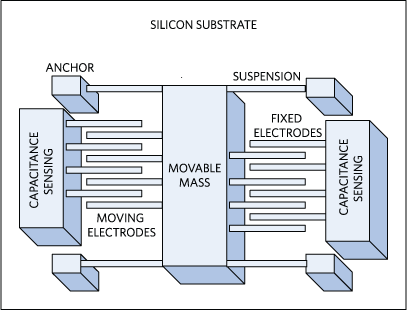
\includegraphics[width=\linewidth]{obrazky/mechmodelaccelerometer.png}\\[0.35em]
                {\small Zjednodušený mechanický model: hmotnosť na pružine s tlmením}
            \end{minipage}
            \caption[Vľavo MEMS akcelerometer, vpravo mechanický model]{Akcelerometer meria zrýchlenie cez silové účinky na vnútornú hmotu. Vľavo princíp MEMS realizácie, vpravo ekvivalent hmotnosť--pružina--tlmenie~\cite{analog_devices_accel_gyro}.}
            \label{fig:accel-principle}
        \end{figure}
      
        \subsection*{Gyroskop}
      
        Na rozdiel od akcelerometra gyroskop meria uhlovú rýchlosť okolo osí, teda rýchlosť zmeny orientácie. Pri dynamickom pohybe preto poskytuje presnejší krátkodobý odhad otočenia než samotný akcelerometer. Ten naopak poskytuje dlhodobejšiu referenciu voči gravitácii. Z tejto vlastnosti vychádza aj motivácia kombinovať obe merania v senzorovej fúzii.
      
        Nevýhodou gyroskopu je postupná akumulácia chyby~\cite{analog_devices_accel_gyro}. Pri autonómnych režimoch, v ktorých robot vykonáva otočky, je preto potrebné počítať s obmedzenou presnosťou pri dlhšom behu. Prakticky sa to môže prejaviť aj tým, že odhad orientácie sa pomaly mení, hoci robot stojí na mieste. V digitálnej implementácii zodpovedá integrácii postupné sčítavanie príspevkov z jednotlivých vzoriek, takže každá malá chyba merania sa postupne kumuluje do odchýlky uhla.
      
        \subsection*{Fúzia senzorových dát (komplementárny filter)}
      
        Samotný akcelerometer aj gyroskop majú svoje obmedzenia, preto sa ich merania kombinujú. Prístup vychádza z princípov komplementárnej filtrácie orientácie~\cite{mahony_filter}, pričom v implementácii používam jednoduchú diskrétnu aproximačnú formu~\cite{complementary_filter_practical}.
      
        Z frekvenčného hľadiska sa tento prístup dá chápať ako hornopriepustná vetva pre gyroskop a dolnopriepustná vetva pre akcelerometer. V diskrétnom kroku $k$ sa najprv z gyroskopu vypočíta prírastok uhla $\omega_k \Delta t$, kde $\omega_k$ je uhlová rýchlosť a $\Delta t$ perióda vzorkovania. Potom sa predikcia z gyroskopu zmieša s uhlom z akcelerometra v bežne používanej aproximačnej forme:
      
        \begin{equation}
          \label{eq:comp-filter}
          \theta_k = \alpha\left(\theta_{k-1} + \omega_k \Delta t\right) + (1-\alpha)\,\theta_{\mathrm{acc},k},
        \end{equation}
      
        kde $\theta_{\mathrm{acc},k}$ je uhol z akcelerometra a parameter $\alpha \in (0,1)$ určuje pomer oboch vetiev. Pri vyššom $\alpha$ má väčšiu váhu gyroskop, čo znamená rýchlejšiu odozvu. Pri nižšom $\alpha$ má väčší vplyv akcelerometer, ktorý viac stabilizuje dlhodobý odhad.
      
        \section{LiDAR a snímač LD19}
      
        Na vnímanie okolia robota je použitý LiDAR senzor. Poskytuje informácie o vzdialenosti prekážok a tieto dáta sú základom pre vyhýbanie sa prekážkam aj pre mapovanie prostredia.
      
        LiDAR (\emph{Light Detection and Ranging}) je optická metóda diaľkového merania~\cite{britannica_lidar}. Z viacerých meraní v rôznych smeroch je možné skladať mapy alebo modely okolia. Používa sa napríklad v presnom mapovaní, archeológii, meteorológii aj v navigácii autonómnych vozidiel.
      
        \begin{figure}[H] 
            \centering
            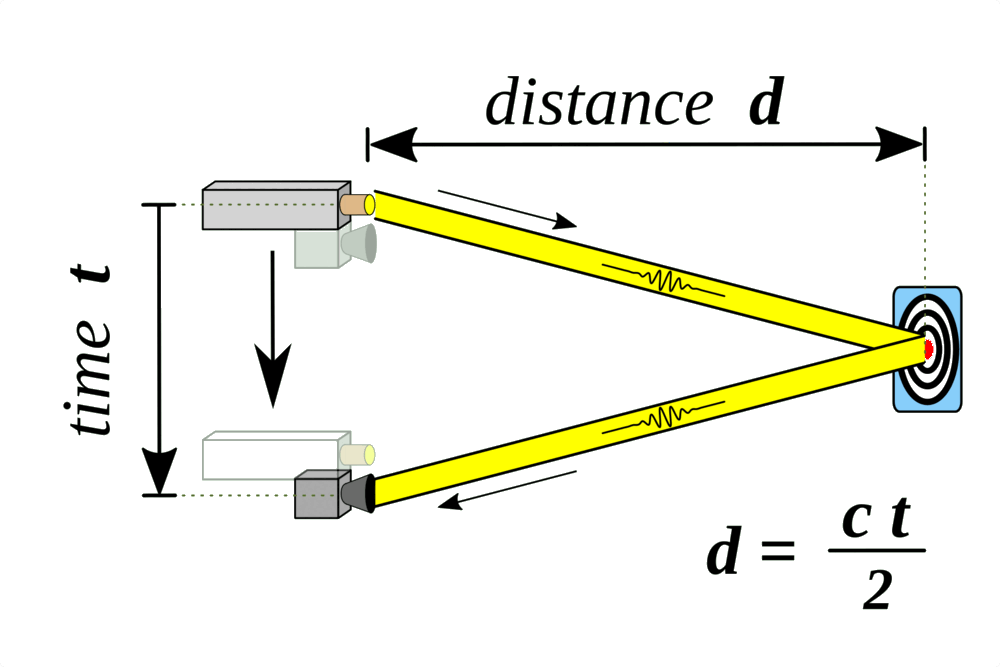
\includegraphics[width=0.6\textwidth]{obrazky/lidar.png} 
            \caption[Princíp LiDAR]{Ilustrácia merania vzdialenosti laserom}
            \label{fig:lidar-principle}
        \end{figure}
      
        Pri rotujúcom LiDARe sa jednotlivé merania vzdialenosti spájajú s uhlom natočenia senzora, čím vzniká dvojrozmerný obraz okolia robota. V ROS~2 sa takýto laserový sken reprezentuje správou \texttt{LaserScan}.
      
        Na Wave Roveri je použitý modul \emph{LD19}\footnote{Dokumentácia snímača DTOF LiDAR LD19: \url{https://www.waveshare.com/wiki/DTOF_LIDAR_LD19}.}. Jeho meracie jadro je založené na princípe \emph{direct time of flight}: laserový impulz sa odrazí od cieľa, prijímač zaznamená čas jeho návratu a z časového intervalu letu sa vypočíta vzdialenosť. Údaje sa následne spájajú s uhlom natočenia a odovzdávajú ako sken.
      
        \section{Raspberry Pi Camera Module 3}
      
        Kamera rozširuje schopnosti robota o vizuálne vnímanie prostredia. Okrem teleprezencie je využívaná pri experimentálnych úlohách, ako je korekcia jazdy a sledovanie farebného objektu.
      
        V práci je použitý oficiálny modul Raspberry Pi Camera Module~3\footnote{Oficiálna dokumentácia Raspberry Pi Camera Module: \url{https://www.raspberrypi.com/documentation/accessories/camera.html}.}. Podrobnejšie technické údaje o rade Camera Module uvádza výrobca v dokumentácii príslušenstva. Snímač využíva Sony IMX708, podporuje HDR snímanie a fázové zaostrovanie, čo uľahčuje ostrenie pri rôznych vzdialenostiach objektov v scéne.
      
        \begin{figure}[H]
            \centering
            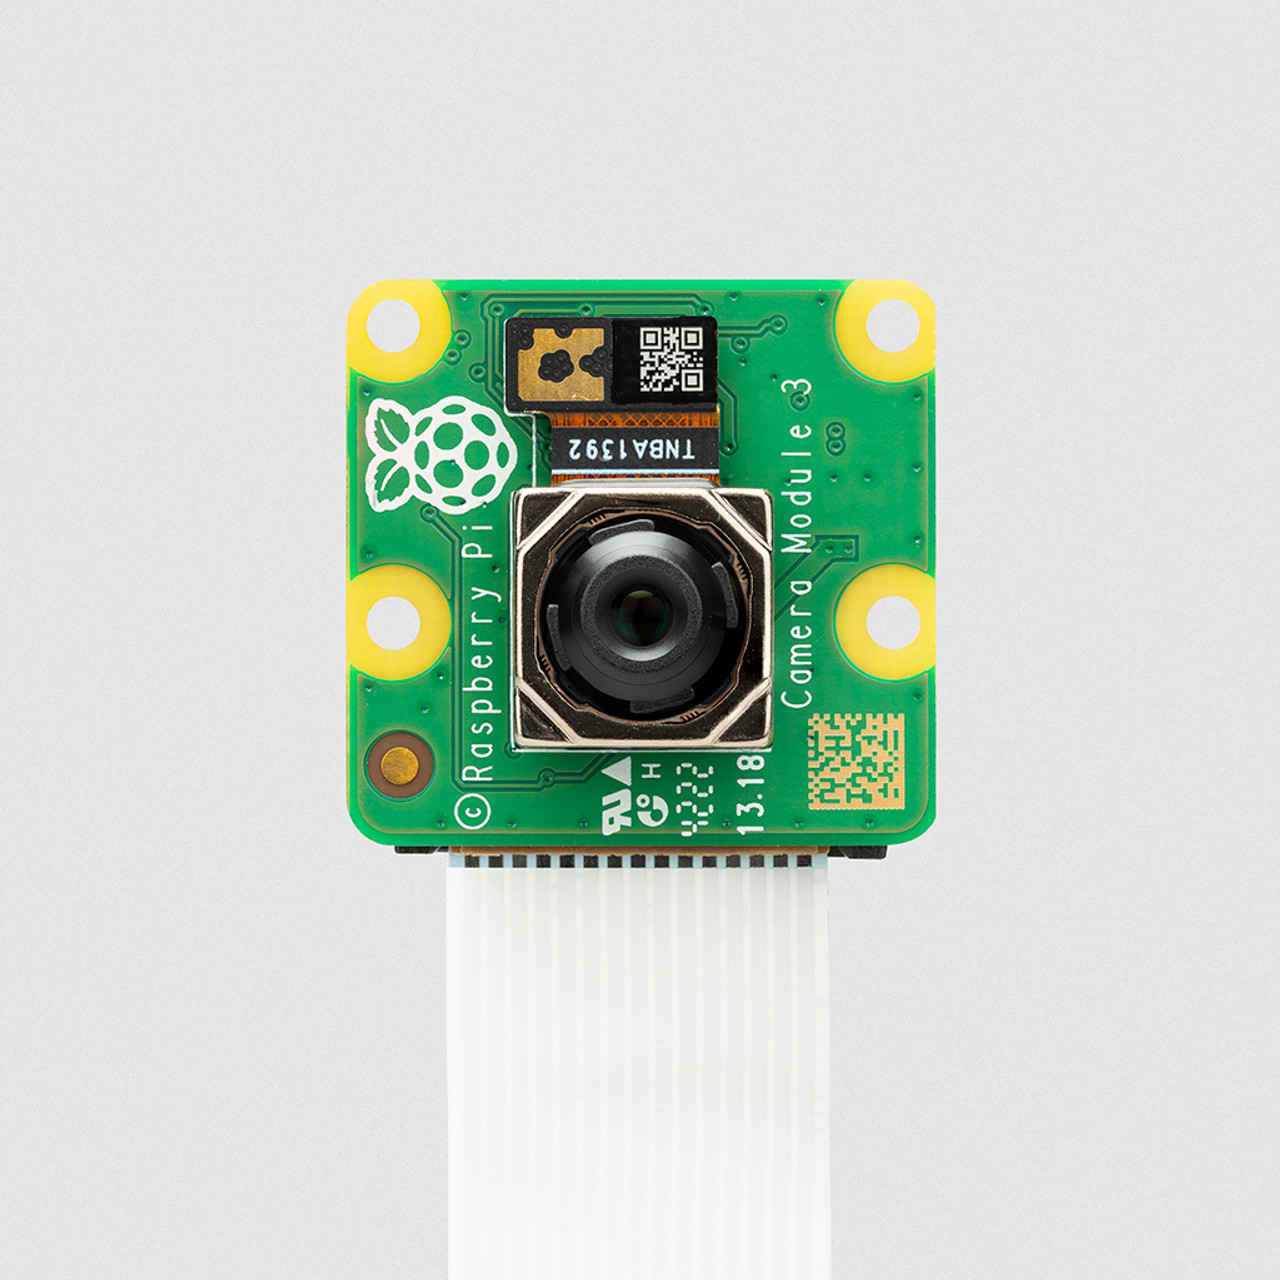
\includegraphics[width=0.4\textwidth]{obrazky/camera_module_3.jpg}
            \caption[Raspberry Pi Camera Module 3]{Raspberry Pi Camera Module~3 (Sony IMX708)}
            \label{fig:camera-module-3-photo}
        \end{figure}
      
        Inštalácia a konfigurácia softvéru (libcamera, balík \texttt{camera\_ros}, témy obrazu v ROS~2) a väzba na ostatné uzly sú podrobnejšie rozobrané v kapitole~\ref{kap:implementacia}, sek.~\ref{sec:kamera-rpi5-ros2}.
      
        \section{Komunikačné rozhrania}
      
        Jednotlivé časti robota musia medzi sebou spoľahlivo komunikovať. Používajú sa najmä dve rozhrania: I\textsuperscript{2}C pre komunikáciu s perifériami na zbernici a UART/USB pre sériový prenos dát medzi mikrokontrolérmi, senzormi a Raspberry Pi. V praxi sa v tejto zostave I\textsuperscript{2}C používa najmä pre krátke prepojenia na doske, zatiaľ čo UART/USB prepojuje samostatné zariadenia.
      
        \subsection*{I\textsuperscript{2}C komunikačné rozhranie}
        \label{sec:i2c}
      
        I\textsuperscript{2}C (\emph{Inter-Integrated Circuit}) je synchronné sériové komunikačné rozhranie určené na prepojenie integrovaných obvodov a periférnych zariadení na spoločnej zbernici. Komunikácia prebieha po dvoch vodičoch: dátovej linke SDA a hodinovej linke SCL, ktorú generuje riadiace zariadenie (master).
      
        Zbernica umožňuje pripojenie viacerých zariadení paralelne, pričom každé zariadenie má vlastnú adresu. Master začne komunikáciu podmienkou START, následne odošle adresu cieľového zariadenia spolu s bitom určujúcim smer prenosu. Dáta sa prenášajú po bajtoch a po každom bajte nasleduje potvrdzovací bit ACK zo strany prijímateľa. Komunikácia je ukončená podmienkou STOP.
      
        Fyzická realizácia zbernice využíva open-drain výstupy~\cite{i2c}. Zariadenia aktívne ťahajú linky k logickej nule, zatiaľ čo logická jednotka je zabezpečená pomocou pull-up rezistorov pripojených na napájacie napätie. Vďaka tomu môže zbernicu zdieľať viac zariadení.
      
        V rámci tejto práce je I\textsuperscript{2}C zbernica využitá najmä na komunikáciu s riadiacim obvodom motorov a inerciálnym senzorom.
      
        \begin{figure}[H] 
            \centering
            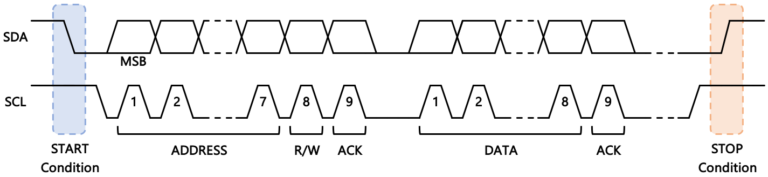
\includegraphics[width=1\textwidth]{obrazky/i2c2.png} 
            \caption{Príklad prenosu dát po I\textsuperscript{2}C}
            \label{fig:i2c-transfer}
        \end{figure}
      
        \subsection*{UART a USB}
      
        UART (\emph{Universal Asynchronous Receiver-Transmitter})~\cite{uart_fundamentals_aticleworld} je asynchrónne sériové rozhranie. Dáta sa prenášajú po jednotlivých bitoch bez zdieľaného hodinového signálu. V mikrokontroléri ide o hardvérovú perifériu, ktorá z paralelných slov procesora vytvára sériový výstup a z prichádzajúceho toku bitov skladá bajty pre CPU.
      
        Obe strany komunikácie musia byť nastavené na rovnakú symbolovú rýchlosť (\emph{baud rate}), ktorá určuje časový úsek jedného bitu. Ak sa rýchlosti nezhodujú, prijímač nesprávne rozdelí rámec a vznikajú chyby. Prenos je najčastejšie dvojlinkový v plnom duplexe: vodič \texttt{TX} jedného zariadenia sa pripája na \texttt{RX} druhého a opačne, pričom obe zariadenia musia mať spoločnú referenčnú zem.
      
        V nečinnom stave je linka v logickej jednotke. Prenos začne štartovým bitom, pri ktorom linka prejde do logickej nuly. Nasledujú dátové bity, prípadne paritný bit a na konci jeden alebo viac stop bitov, ktoré vrátia linku späť do pokojového stavu. Prijímač sa zosynchronizuje podľa prechodu štartového bitu a následne číta jednotlivé bity v pravidelných intervaloch.
      
        \begin{figure}[H] 
            \centering
            \IfFileExists{obrazky/uart.png}{%
                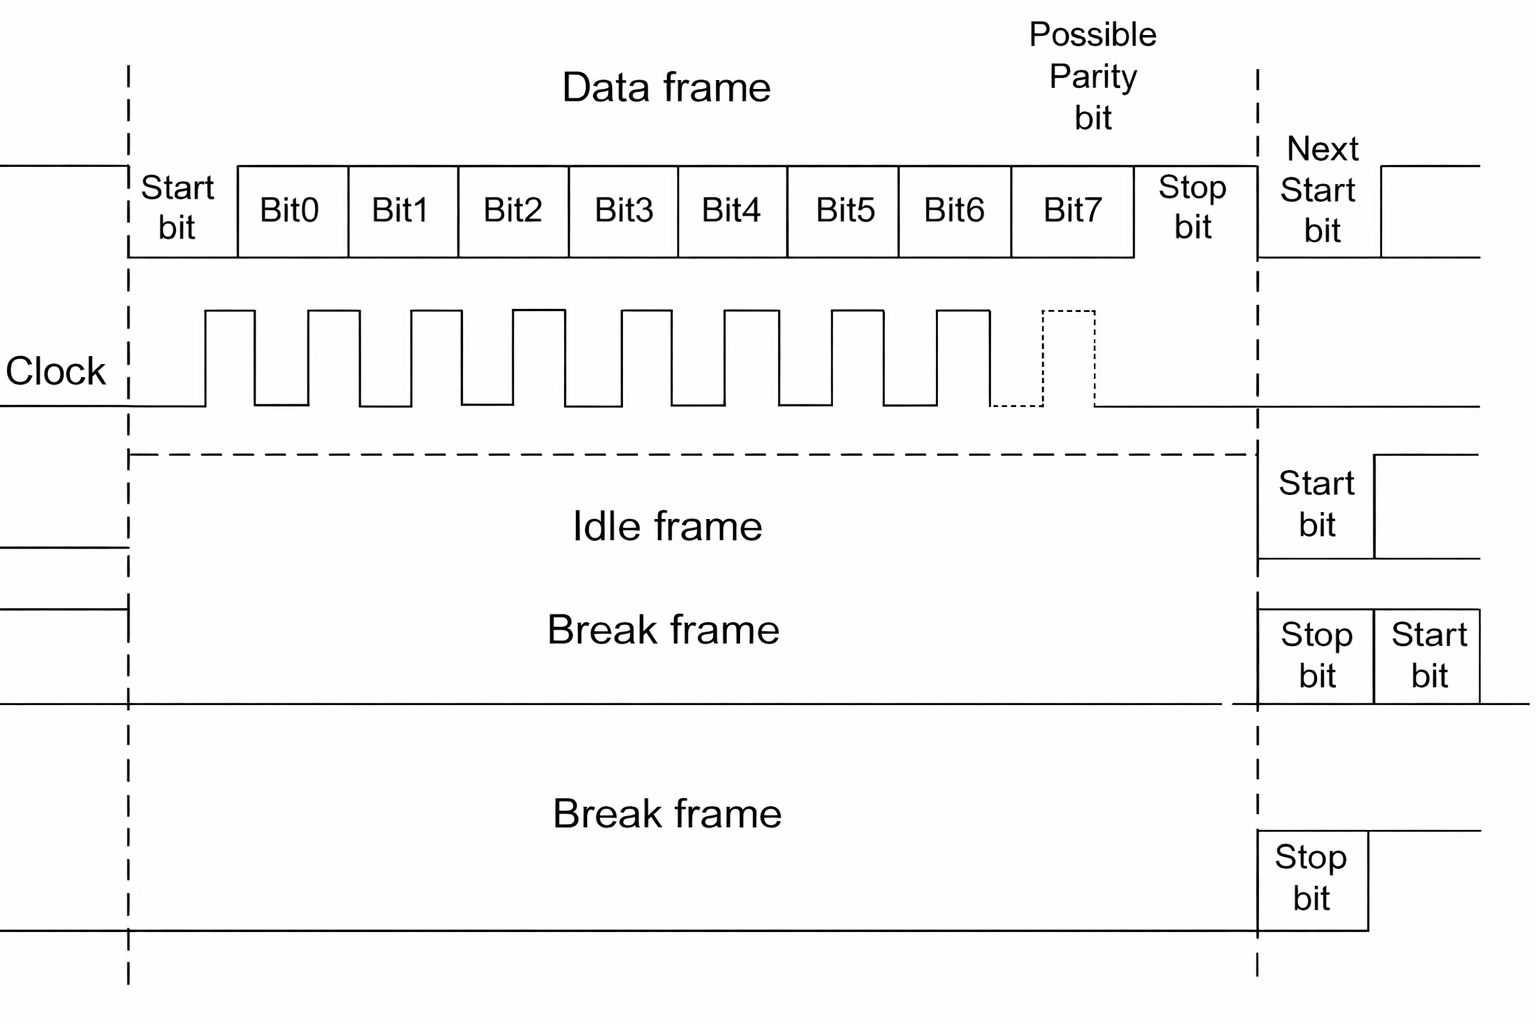
\includegraphics[width=0.8\textwidth]{obrazky/uart.png}%
            }{%
                \fbox{\begin{minipage}{0.78\textwidth}\centering\small
                    Chýba súbor \texttt{obrazky/uart.png} (časový diagram UART). Po doplnení obrázka zmizne tento rámček.
                \end{minipage}}%
            }
            \caption[Časový diagram UART]{Časový diagram UART: rámec so štartovým bitom, dátovými bitmi, voliteľnou paritou a stop bitom.}
            \label{fig:uart-timing}
        \end{figure}
      
      
        \chapter{Robot Operating System 2}
      
        ROS~2 v navrhnutom riešení slúži ako komunikačná vrstva medzi motorovým uzlom, senzormi, kamerou, webovým rozhraním, simuláciou a autonómnymi modulmi. Aby bolo jasné, ako sú jednotlivé časti prepojené, táto kapitola stručne predstavuje koncepty ROS~2, ktoré sa priamo využívajú pri implementácii robota.
      
        Najprv je opísaná základná architektúra ROS~2 a komunikácia. Ďalej sú vysvetlené uzly, témy, služby, akcie a parametre, teda prvky, z ktorých je zložená výsledná zostava. Záver kapitoly sa venuje nástrojom na ladenie, transformáciám a simulácii, ktoré boli použité pri vývoji a overovaní riešenia.
      
        \section{Úvod, architektúra a zdroje informácií}
      
        ROS~2 je middleware platforma určená na vývoj robotických aplikácií. Ide o sadu knižníc, nástrojov a rozhraní, ktoré zjednocujú komunikáciu medzi komponentmi robotického systému. ROS~2 poskytuje štandardizovaný spôsob práce s uzlami, správami, témami, službami, akciami, parametrami a transformáciami, čím uľahčuje návrh modulárnych a distribuovaných aplikácií.
      
        V porovnaní s ROS1 je navrhnutý na robustnejšie nasadenie v distribuovaných systémoch, podporu viacerých platforiem a flexibilnejšiu komunikáciu cez DDS. Architektúra oddeľuje aplikačný kód od transportnej vrstvy a umožňuje meniť middleware bez zásahu do logiky uzlov.
      
        Väčšina tejto kapitoly vychádza z oficiálnej dokumentácie ROS~2~\cite{ros2_doc}, takže priebežné vysvetlenia a príklady budú spracované na základe tohto zdroja.
      
        \begin{figure}[H]
            \centering
            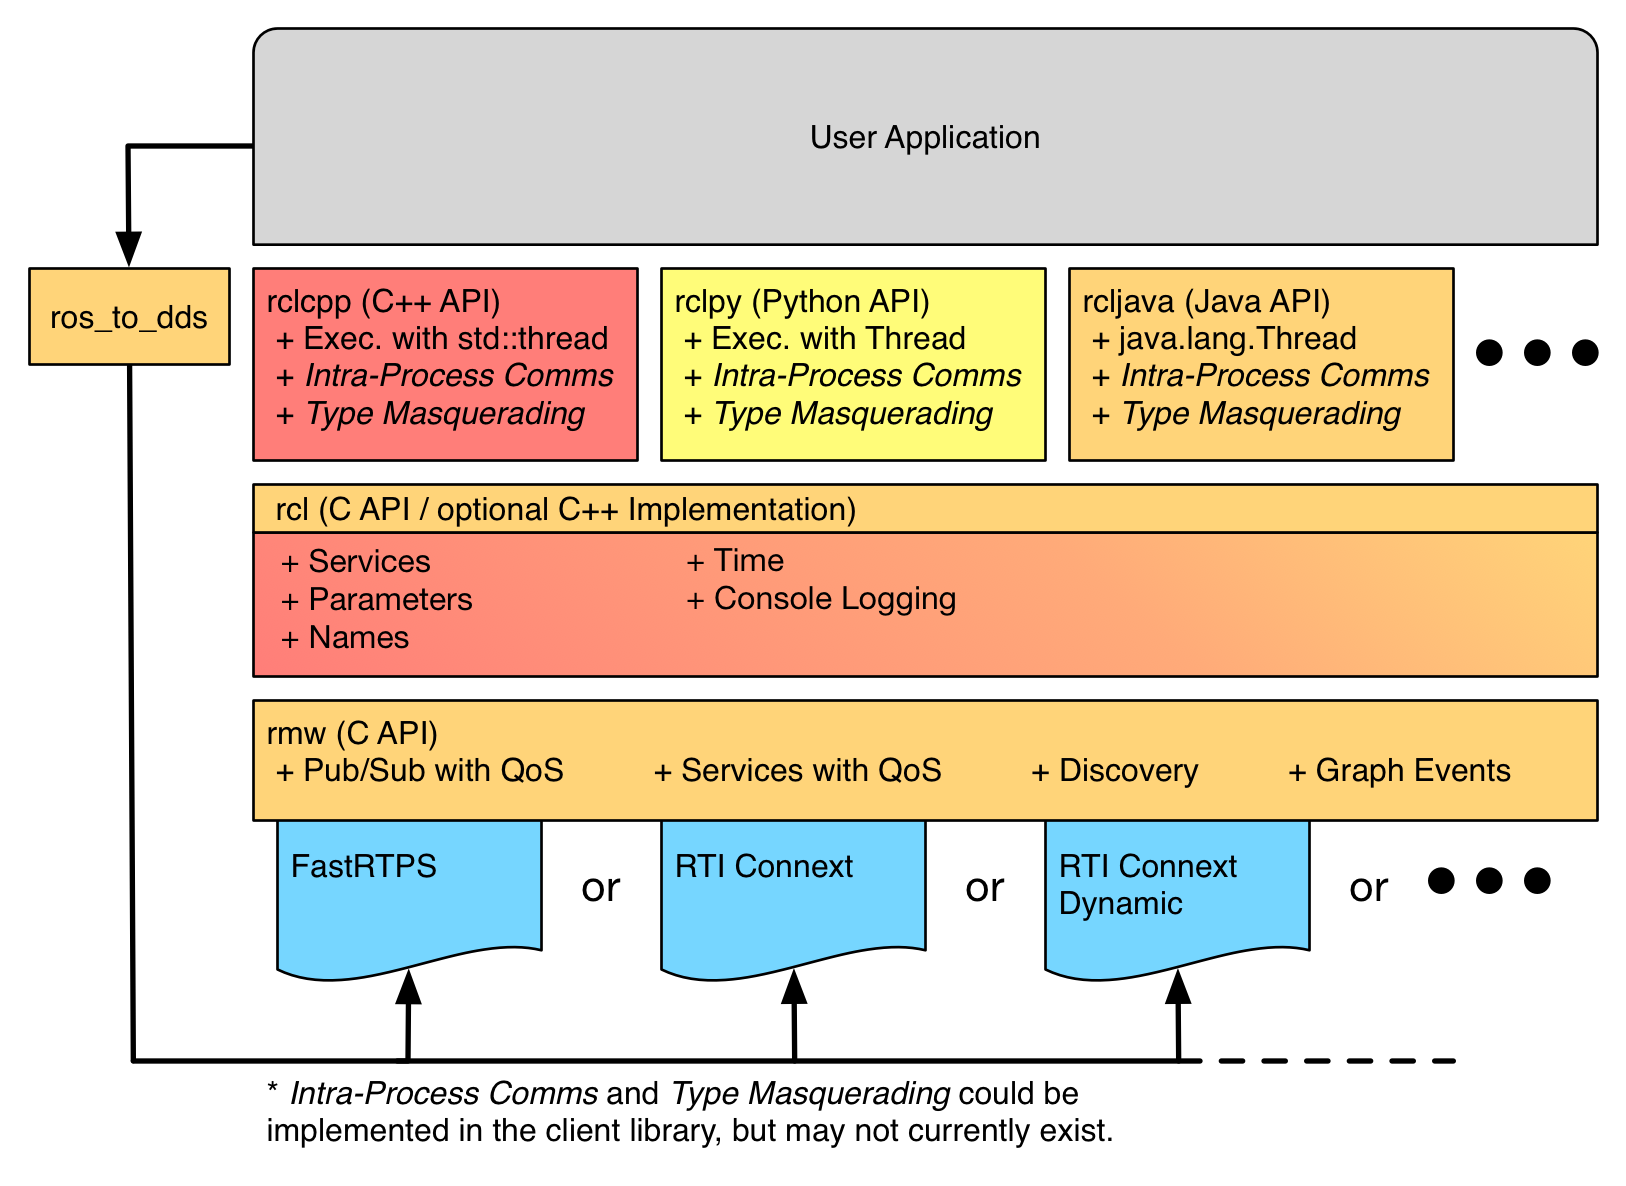
\includegraphics[width=0.88\textwidth]{obrazky/ros_client_library_api_stack.png}
            \caption[Zásobník klientskych knižníc ROS~2]{Zásobník klientskych knižníc a rozhraní: aplikácia cez \texttt{rclpy}/\texttt{rclcpp}, spoločná vrstva RCL, RMW a DDS ako transport }
            \label{fig:ros2-client-library-stack}
        \end{figure}
      
        \section{DDS, domény a micro-ROS}
      
        V tomto riešení beží zostava distribuovane medzi Raspberry Pi a externým počítačom. V krátkosti vysvetlím, ako ROS~2 zabezpečuje komunikáciu medzi uzlami v sieti a ako sa jednotlivé behy oddeľujú pomocou domén.
      
        \subsection*{DDS a discovery}
      
        Komunikačný základ ROS~2 tvorí DDS~\cite{dds_foundation_what_is_dds}, čo je decentralizovaný publish--subscribe middleware. DDS zabezpečuje priamu komunikáciu medzi uzlami bez centrálneho servera. Po spustení uzla dochádza k jeho automatickému oznámeniu v rámci rovnakej domény. Následne sa vytvorí spojenie s kompatibilnými účastníkmi komunikácie.
      
        Výber, ktorá logická DDS doména sa použije, sa riadi premennou prostredia \texttt{ROS\_DOMAIN\_ID}. Uzly so zhodným ID patria do jednej skupiny pre discovery a výmenu správ, odlišná hodnota oddelí napríklad viac nezávislých behov ROS~2 na jednom počítači alebo susedné robotické systémy v lokálnej sieti.
      
        \subsection*{micro-ROS a embedded systémy}
      

        Pre mikrokontroléry s obmedzenou pamäťou a výkonom nie je plný ROS~2 stack na zariadení reálny a preto v ekosystéme existuje \emph{micro-ROS}\footnote{Oficiálna dokumentácia micro-ROS: \url{https://micro.ros.org/}.}. Ide o zjednodušené klientské knižnice, ktoré na MCU zachovávajú základné koncepty ROS~2 (uzly, témy, služby, parametre). Typicky beží \emph{micro-ROS klient} na zariadení ako ESP32 či STM32 a \emph{micro-ROS agent} na výkonnejšom uzle zabezpečí premostenie do tej istej DDS domény ako ostatné uzly.
      
        \section{Uzly, správy a priebežná komunikácia}
      
        Výsledný systém je rozdelený na viacero samostatných uzlov, z ktorých každý rieši konkrétnu úlohu, napríklad čítanie senzora, riadenie motorov alebo spracovanie obrazu. Ďalej ukazujem tento komunikačný model ROS~2.
      
        \subsection*{Uzly a klientské knižnice}
      
        Základnou jednotkou aplikácie je uzol (\emph{node}). Uzol, ako som hovoril v úvode, predstavuje samostatný proces alebo logickú časť procesu, ktorá vykonáva určitú funkcionalitu. 
      
        Nasledujúca ukážka ilustruje najjednoduchšiu kostru uzla v \texttt{rclpy}:
      
        \begin{verbatim}
        import rclpy
        from rclpy.node import Node
      
        class SimpleNode(Node):
            def __init__(self):
                super().__init__('simple_node')
                self.get_logger().info('Uzol bol spustený')
      
        def main(args=None):
            rclpy.init(args=args)
            node = SimpleNode()
            rclpy.spin(node)
            node.destroy_node()
            rclpy.shutdown()
        \end{verbatim}
      
        \subsection*{Správy a rozhrania}
      
        Komunikácia medzi uzlami prebieha pomocou správ (\emph{messages}), ktorých formát je pevne definovaný rozhraním. Štandardné typy správ sú súčasťou balíkov ako \texttt{std\_msgs}, \texttt{geometry\_msgs}, \texttt{sensor\_msgs} alebo \texttt{nav\_msgs} (definície typov sú súčasťou ekosystému ROS~2).
      
        Pre túto prácu sú dôležité napríklad typy:
        \begin{itemize}
            \item \texttt{sensor\_msgs/msg/LaserScan} pre 2D lidar,
            \item \texttt{sensor\_msgs/msg/Image} pre kameru,
            \item \texttt{sensor\_msgs/msg/Imu} pre IMU,
            \item \texttt{geometry\_msgs/msg/Twist} pre rýchlostné príkazy,
            \item \texttt{nav\_msgs/msg/Odometry} pre odometriu.
        \end{itemize}
      
        \subsection*{Témy a model publisher--subscriber}
      
        Témy (\emph{topics}) sú asynchrónne komunikačné kanály určené na priebežnú výmenu správ medzi uzlami. Publisher odosiela správy na tému a subscriber ich prijíma. Tento model je vhodný pre kontinuálne dátové toky zo senzorov alebo z riadiacich uzlov.
      
        Príklad jednoduchého publishera v jazyku Python:
      
        \begin{verbatim}
        from std_msgs.msg import String
        import rclpy
        from rclpy.node import Node
      
        class Talker(Node):
            def __init__(self):
                super().__init__('talker')
                self.pub = self.create_publisher(String, 'demo_topic', 10)
                self.timer = self.create_timer(0.5, self.timer_callback)
                self.counter = 0
      
            def timer_callback(self):
                msg = String()
                msg.data = f'Sprava {self.counter}'
                self.pub.publish(msg)
                self.counter += 1
        \end{verbatim}
      
        Zodpovedajúci subscriber môže mať tvar:
      
        \begin{verbatim}
        from std_msgs.msg import String
        import rclpy
        from rclpy.node import Node
      
        class Listener(Node):
            def __init__(self):
                super().__init__('listener')
                self.sub = self.create_subscription(
                    String, 'demo_topic', self.callback, 10)
      
            def callback(self, msg):
                self.get_logger().info(f'Prijata sprava: {msg.data}')
        \end{verbatim}
      
        \begin{figure}[H]
            \centering
            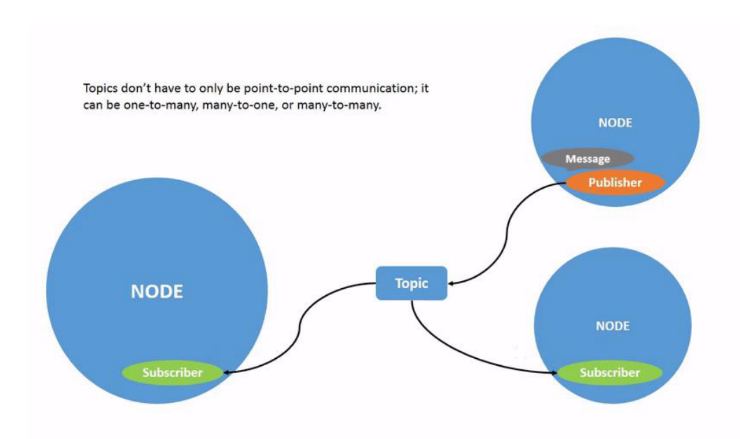
\includegraphics[width=0.7\textwidth]{obrazky/publisher_subscriber.png}
            \caption[Model publisher a subscriber na téme]{Publisher publikuje správy na tému a jeden alebo viac subscriberov ich odoberá}
            \label{fig:ros2pubsub}
        \end{figure}
      
        \section{Služby, akcie a kvalita služieb}
      
        Nie všetka komunikácia má rovnaký charakter. Senzorické dáta sa posielajú priebežne, prepnutie režimu je jednorazová požiadavka a sledovanie lopty je dlhšie trvajúca úloha. Preto ROS~2 rozlišuje témy, služby a akcie.
      
        \subsection*{Služby}
      
        Služby (\emph{services}) realizujú synchrónny model request--response. Klient odošle požiadavku a server vráti odpoveď. Tento spôsob komunikácie sa používa na jednorazové operácie, ktoré majú mať jednoznačný výsledok, ako je reset modulu, prepnutie režimu alebo získanie konfigurácie.
      
        Zjednodušený príklad servera služby:
      
        \begin{verbatim}
        from example_interfaces.srv import AddTwoInts
        import rclpy
        from rclpy.node import Node
      
        class AddService(Node):
            def __init__(self):
                super().__init__('add_service')
                self.srv = self.create_service(
                    AddTwoInts, 'add_two_ints', self.callback)
      
            def callback(self, request, response):
                response.sum = request.a + request.b
                return response
        \end{verbatim}
      
        \subsection*{Akcie}
      
        Akcie (\emph{actions}) sú určené pre dlhšie trvajúce operácie. Na rozdiel od služieb umožňujú priebežnú spätnú väzbu, vrátenie konečného výsledku a zrušenie požiadavky. Využívajú napríklad pri navigácii, manipulácii alebo vykonávaní komplexnej sekvencie pohybov.
      
        Typická akcia zahŕňa:
        \begin{itemize}
            \item odoslanie cieľa (\emph{goal}),
            \item priebežný feedback,
            \item finálny výsledok (\emph{result}).
        \end{itemize}
      
        Zjednodušená myšlienka callbacku akčného servera:
      
        \begin{verbatim}
        def execute_callback(self, goal_handle):
            sequence = [0, 1]
            for i in range(2, goal_handle.request.order):
                sequence.append(sequence[i-1] + sequence[i-2])
                goal_handle.publish_feedback(...)
            goal_handle.succeed()
            result = Fibonacci.Result()
            result.sequence = sequence
            return result
        \end{verbatim}
      
        \subsection*{QoS}
      
        Dôležitou vlastnosťou ROS~2 je podpora Quality of Service (QoS), ktorá umožňuje ovplyvniť správanie komunikácie medzi uzlami. Pomocou QoS je možné nastaviť, či je pri prenose dát dôležitejšia spoľahlivosť (aby sa nestratili správy), alebo nízka latencia (aby boli dáta čo najaktuálnejšie).
      
        Medzi najdôležitejšie QoS politiky patria:
        \begin{itemize}
            \item \textbf{history} a \textbf{depth} – určujú, koľko posledných správ sa uchováva v pamäti,
            \item \textbf{reliability} – definuje, či má byť prenos spoľahlivý (bez straty dát) alebo najlepšou snahou (môžu sa stratiť niektoré správy),
            \item \textbf{durability} – určuje, či noví odberatelia dostanú aj staršie správy,
            \item \textbf{deadline} – maximálny čas medzi správami,
            \item \textbf{lifespan} – ako dlho je správa platná,
            \item \textbf{liveliness} – mechanizmus na kontrolu, či je uzol stále aktívny.
        \end{itemize}
      
        Voľba QoS závisí od konkrétneho použitia. Zo skúsenosti sa osvedčilo, že pri senzorických dátach, ako sú dáta z LiDARu alebo kamery, je lepšie uprednostniť aktuálnosť než úplnú spoľahlivosť a vybrať režim \emph{best effort}. Pri riadiacich príkazoch je zasa vhodnejšie použiť spoľahlivý prenos.
      
        \section{Workspace, balíky, build, launch a parametre}
      
        Keďže systém pozostáva z viacerých balíkov a uzlov, bolo potrebné riešiť aj ich organizáciu, spúšťanie a konfiguráciu. Na to slúži ROS~2 workspace, launch súbory a parametre.
      
        \subsection*{Workspace, balíky a build systém}
      
        Vývoj v ROS~2 prebieha vo workspace, ktorého zdrojová časť sa spravidla nachádza v priečinku \path{src/}. Po príkaze \texttt{colcon build} vznikajú priečinky \path{build/}, \path{install/} a \path{log/}. Dokumentácia Jazzy rozlišuje aj vzťah \emph{underlay} a \emph{overlay}, kde systémová inštalácia ROS~2 tvorí základ a vlastný workspace na ňu nadväzuje.
      
        Príklad typickej štruktúry Python balíka:
      
        \begin{verbatim}
        my_package/
        |-- package.xml
        |-- setup.py
        |-- setup.cfg
        |-- resource/
        |-- my_package/
        |   |-- __init__.py
        |   `-- my_node.py
        |-- launch/
        `-- config/
        \end{verbatim}
      
        \subsection*{Launch súbory}
      
        Launch súbory slúžia na spustenie viacerých uzlov, nastavenie parametrov, remapovanie tém a celkové zostavenie aplikácie. V ROS~2 sa bežne používajú Python launch súbory, ktoré vracajú objekt \texttt{LaunchDescription}.
      
        Jednoduchý launch súbor môže vyzerať nasledovne:
      
        \begin{verbatim}
        from launch import LaunchDescription
        from launch_ros.actions import Node
      
        def generate_launch_description():
            return LaunchDescription([
                Node(
                    package='demo_nodes_py',
                    executable='talker',
                    name='demo_talker'
                )
            ])
        \end{verbatim}
      
        \subsection*{Parametre}
      
        Parametre sú konfiguračné hodnoty viazané na konkrétny uzol. Možno ich nastavovať pri štarte aj za behu a ich životnosť sa viaže na životnosť uzla.
      
        Príklad deklarácie a čítania parametra v \texttt{rclpy}:
      
        \begin{verbatim}
        import rclpy
        from rclpy.node import Node
      
        class ParamNode(Node):
            def __init__(self):
                super().__init__('param_node')
                self.declare_parameter('gain', 0.5)
                gain = self.get_parameter('gain').value
                self.get_logger().info(f'gain = {gain}')
        \end{verbatim}
      
        Parametre sa zvyknú ukladať do YAML súborov a predávajú cez launch súbory, čo zjednodušuje konfiguráciu viacerých uzlov bez zásahu do zdrojového kódu.
      
        \section{Nástroje ladenia, transformácie a vizualizácia}
      
        Pri vývoji robota nestačilo uzly iba spustiť, bolo potrebné aj sledovať, či medzi sebou správne komunikujú a či dáta zo senzorov dávajú zmysel. Preto boli pri práci užitočné nástroje na introspekciu, vizualizáciu a ladenie.
      
        \subsection*{Príkazový riadok a introspekcia systému}
      
        ROS~2 obsahuje rozsiahle CLI nástroje na introspekciu systému, ktoré umožňujú sledovať stav uzlov, komunikáciu a konfiguráciu bez zásahu do kódu. Medzi najdôležitejšie patria:
        \begin{itemize}
            \item \texttt{ros2 node list} -- zobrazí zoznam všetkých aktívnych uzlov v systéme, \texttt{ros2 node info} poskytne detailné informácie o konkrétnom uzle (publikované a odoberané témy, služby),
            
            \item \texttt{ros2 topic list} -- vypíše dostupné témy, \texttt{ros2 topic echo} umožňuje sledovať obsah správ publikovaných na téme, \texttt{ros2 topic hz} odhaduje frekvenciu publikovania,
            
            \item \texttt{ros2 service list} -- zobrazí dostupné služby, \texttt{ros2 service call} umožňuje manuálne zavolať službu s konkrétnymi parametrami,
            
            \item \texttt{ros2 param list} -- vypíše parametre uzlov, \texttt{ros2 param get} a \texttt{ros2 param set} slúžia na čítanie a zmenu hodnôt parametrov počas behu,
            
            \item \texttt{ros2 interface show} -- zobrazí definíciu typu správy, služby alebo akcie (napr.\ štruktúru \texttt{sensor\_msgs/msg/LaserScan}),
            
            \item \texttt{ros2 doctor} -- diagnostický nástroj, ktorý kontroluje správnosť konfigurácie ROS~2 prostredia a upozorňuje na možné problémy.
        \end{itemize}
      
        \subsection*{tf2 a súradnicové rámce}
      
        Subsystém tf2 slúži na reprezentáciu vzťahov medzi súradnicovými rámami robota. Každá transformácia má rodičovský a detský rám, čím vzniká strom transformácií. Bežne sa používajú rámce ako \path{map}, \path{odom}, \path{base_link} alebo rámce jednotlivých senzorov. Robot to potrebuje na správne prepočty polohy medzi mapou, podvozkom a senzormi.
      
        Statické transformácie opisujú pevné geometrické vzťahy, napríklad montáž senzora na podvozok. Dynamické transformácie sa menia v čase, čo je napríklad poloha robota voči odometrii. V \texttt{rclpy} sa na publikovanie transformácií používa \texttt{TransformBroadcaster} a na ich odoberanie kombinácia \texttt{Buffer} a \texttt{TransformListener}.
      
        \begin{figure}[H]
            \centering
            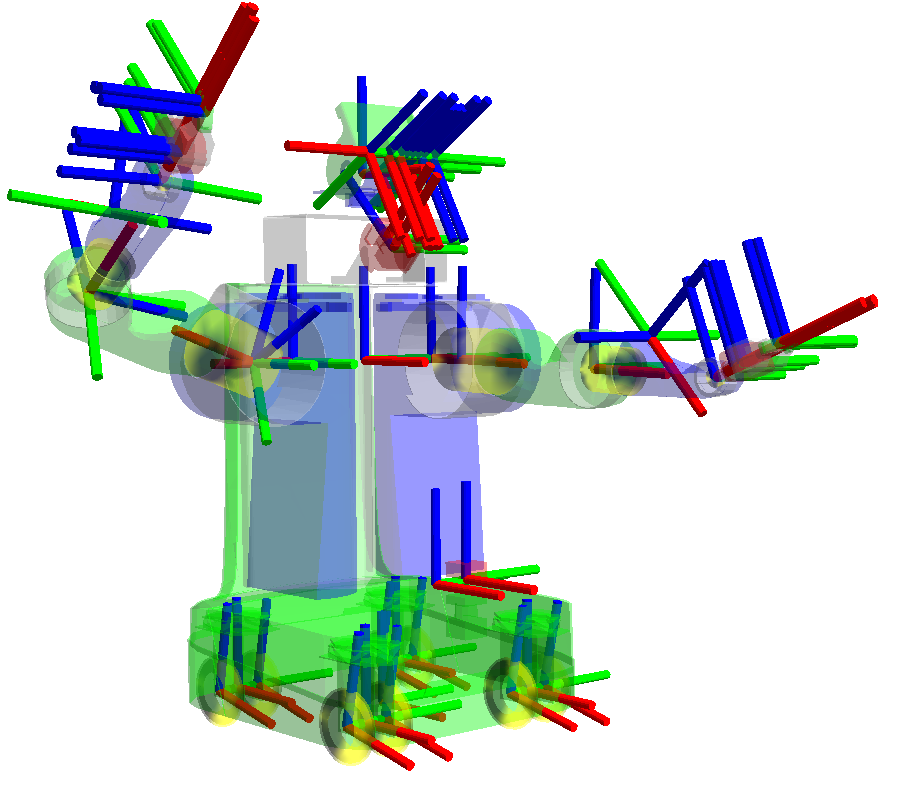
\includegraphics[width=0.45\textwidth]{obrazky/ros2_tf2_frames.png}
            \caption[Strom súradnicových rámov tf2]{Príklad stromu súradnicových rámov prepojených transformáciami tf2, rodičovské a detské rámce zodpovedajú vzťahom medzi mapou, odometriou, podvozkom a senzormi}
            \label{fig:ros2-tf2-frames}
        \end{figure}
      
        \subsection*{RViz2 a rqt}
      
        RViz2 je hlavný vizualizačný nástroj v prostredí ROS~2, ktorý umožňuje zobrazenie stavu robota a dát zo senzorov v reálnom čase. Podporuje vizualizáciu 3D modelu robota, laserových skenov, obrazových dát, markerov, máp, plánovaných trajektórií a transformácií medzi súradnicovými rámami. Dá sa v ňom dynamicky pridávať jednotlivé zobrazovacie prvky a konfigurovať ich parametre podľa potreby.
        V rámci tejto práce sa využíva RViz na výkonnejšom externom počítači~\ref{sec:distrib-slam-rviz}.
      
        Balík rqt združuje sadu grafických nástrojov, ktoré slúžia na analýzu a ladenie systému. Medzi najčastejšie používané patria:
        \begin{itemize}
            \item \texttt{rqt\_graph} -- zobrazuje graf uzlov a tém, čo umožňuje overiť štruktúru komunikácie a prepojenie jednotlivých komponentov,
            
            \item \texttt{rqt\_plot} -- umožňuje sledovať časový priebeh číselných veličín publikovaných na témach, napríklad výstupy regulátora alebo hodnoty zo senzorov,
            
            \item \texttt{rqt\_image\_view} -- slúži na zobrazenie obrazových dát zo senzorov, napríklad kamery alebo spracovaného obrazu.
        \end{itemize}
      
      \section{Simulácia robotických systémov}
      
      Simuláciu som využil na overenie modelu robota, senzorov a správania ešte pred nasadením na fyzický hardvér. Detailnejšie nastavenie a konkrétne použitie uvádzam v kapitole o implementácii.
      
      \subsection*{Gazebo a simulácia}
      
      ROS~2 podporuje simuláciu robotických systémov prostredníctvom nástrojov, ako je Gazebo Sim~\cite{gazebo}. Pred samotnou prácou s hardvérom som v simulácii testoval algoritmy aj so simulovanými senzormi a fyzikou prostredia.
      
      Prepojenie medzi ROS~2 a Gazebo Sim sa rieši pomocou balíkov \texttt{ros\_gz\_sim} a \texttt{ros\_gz\_bridge}, ktoré zabezpečujú komunikáciu medzi simulačným prostredím a ROS témami.
      
      Konkrétnu konfiguráciu a spôsob využitia týchto nástrojov podrobnejšie opisujem v kapitole~\ref{kap:implementacia}, najmä v sekcii~\ref{sec:sim-gazebo}.
      
        \chapter{Implementácia}
        \label{kap:implementacia}
      
        V tejto kapitole sa venujem návrhu a realizácii výsledného systému. Postupne prejdem prípravu vývojového prostredia, modelovanie robota so simulačnou vrstvou, konfiguráciu s pôvodným driverom a nakoniec hlavnú implementáciu.
      
          Neopisujem len samotné implementačné kroky, ale aj to, ako sú jednotlivé časti navrhnuté, aby spolu fungovali ako modulárny a rozšíriteľný systém.
      
        Pri vypracovaní tejto bakalárskej práce som sa čiastočne inšpiroval bakalárskou prácou Daniela Onderku~\cite{onderka2024mobilecamera} z hľadiska štruktúry textu a taktiež pri niektorých implementačných prvkoch: režim blúdenia (wander), jednoduchá bodová navigácia a Gazebo simulácia.
      
      
        \section{Hardvérová a systémová príprava}
        \label{sec:setup-pred-spojazdnenim}
      
        Ešte pred samotným spojazdnením robota bolo potrebné pripraviť jednotné prostredie na Raspberry Pi. Ako základ softvérového stacku je operačný systém Ubuntu~24.04 a k nemu distribúcia ROS~2 Jazzy. Súčasťou prípravy bolo aj nastavenie ROS\_DOMAIN\_ID, ktoré zabezpečuje, aby uzly bežiace na rôznych zariadeniach patrili do rovnakej komunikačnej domény a mohli si medzi sebou vymieňať správy.
      
        Osobitnú pozornosť si vyžadovala integrácia kamery na Raspberry Pi~5. Podrobný opis problémov s \path{/dev/video*}, vrstvou \emph{libcamera} a voľbou balíka \texttt{camera\_ros}\footnote{Praktický postup pre RPi5 a ROS~2 Jazzy: \url{https://github.com/ARLunan/Raspberry-Pi-Camera-ROS/blob/main/Documents/RPCamera-Installation-RP5.md}. Oficiálny repozitár \texttt{camera\_ros}: \url{https://github.com/christianrauch/camera_ros}.} je uvedený v sekcii~\ref{sec:kamera-rpi5-ros2}. V tejto časti chcem len spomenúť, že pre stabilnú prevádzku sa osvedčil práve tento prístup.
      
        \section{Model robota a simulačná vrstva}
        \label{sec:sim-gazebo}
      
        Súčasťou návrhu systému bolo vytvorenie jednotného modelu robota. Vytvorenie modelu robota je dôležité pre simulácie, vďaka čomu sa dajú testovať algoritmy ešte skôr, ako spustím reálneho robota.
      
        Model je vytvorený vo formáte Xacro a rozdelený na viacero logických častí. Základ tvorí telo robota reprezentované rámom \texttt{base\_link}, ku ktorému sú pripojené kolesá a jednotlivé senzorické bloky. Pri definovaní modelu nebola doplnená len vizuálna reprezentácia, ale aj kolízne a zotrvačné parametre, aby model neslúžil iba na zobrazenie, ale aj na fyzikálnu simuláciu v Gazebo.
      
        \subsection{Definícia tela}
      
        Podvozok som definoval ako jednoduchý kváder s príslušnou hmotnosťou, geometriou a aproximačnou maticou zotrvačnosti:
      
        \begin{verbatim}
        <link name="base_link">
            <inertial>
                <mass value="1.2"/>
                <origin xyz="0 0 0"/>
                <inertia ixx="0.003" iyy="0.005" izz="0.006"/>
            </inertial>
            <visual>
                <origin xyz="0 0 0"/>
                <geometry><box size="${body_l} ${body_w} ${body_h}"/></geometry>
                <material name="dark_gray"/>
            </visual>
            <collision>
                <origin xyz="0 0 0"/>
                <geometry><box size="${body_l} ${body_w} ${body_h}"/></geometry>
            </collision>
        </link>
        \end{verbatim}
      
        Hodnoty zotrvačnosti v ukážke vyššie nezodpovedajú presnému rozloženiu na reálnom podvozku, no presné hodnoty by si vyžadovali detailnejšie meranie rozloženia hmotnosti, čo presahuje rámec tejto práce. Aktuálne hodnoty teda postačia.
      
        Kolesá sú k telu podvozku pripojené rotačnými kĺbmi. V simulačnej vrstve boli doplnené aj základné parametre kontaktu a trenia, aby sa správanie modelu aspoň približne podobalo fyzickému podvozku.
      
        \subsection{Kamera a LiDAR}
      
        Na ten istý základný rám boli pomocou pevných kĺbov pripojené aj kamera a LiDAR.
      
        \begin{verbatim}
        <joint name="camera_joint" type="fixed">
            <parent link="base_link"/>
            <child link="camera_link"/>
            <origin xyz="0.097 0 0.005" rpy="0 0 0"/>
        </joint>
        <joint name="lidar_joint" type="fixed">
            <parent link="base_link"/>
            <child link="lidar_link"/>
            <origin xyz="-0.04 0 0.092" rpy="0 0 0"/>
        </joint>
        \end{verbatim}
      
        \subsection{Gazebo Sim a RViz2}
      
        Takto pripravený model bol následne použitý v RViz2 aj v Gazebo Sim~\cite{gazebo} -- vizualizácia aj fyzikálna simulácia vychádzajú z tej istej štruktúry. V simulačnom prostredí sú kamera aj LiDAR sprístupnené cez \path{ros_gz_bridge}, vďaka čomu s nimi viem pracovať ako so štandardnými ROS témami, napríklad \rostopic{/camera/image_raw} a \rostopic{/scan}.
      
        Simulácia mi umožnila prvotné vyskúšanie manuálneho aj autonómneho riadenia robota, vrátane experimentov s navigáciou v štýle Nav2 v simulácii. Oproti reálnemu prostrediu však pretrvávajú rozdiely v trení, poddajnosti kolies, oneskorení senzorov a šume.
      
        \begin{figure}[H]
            \centering
            \begin{minipage}[t]{0.49\textwidth}
                \centering
                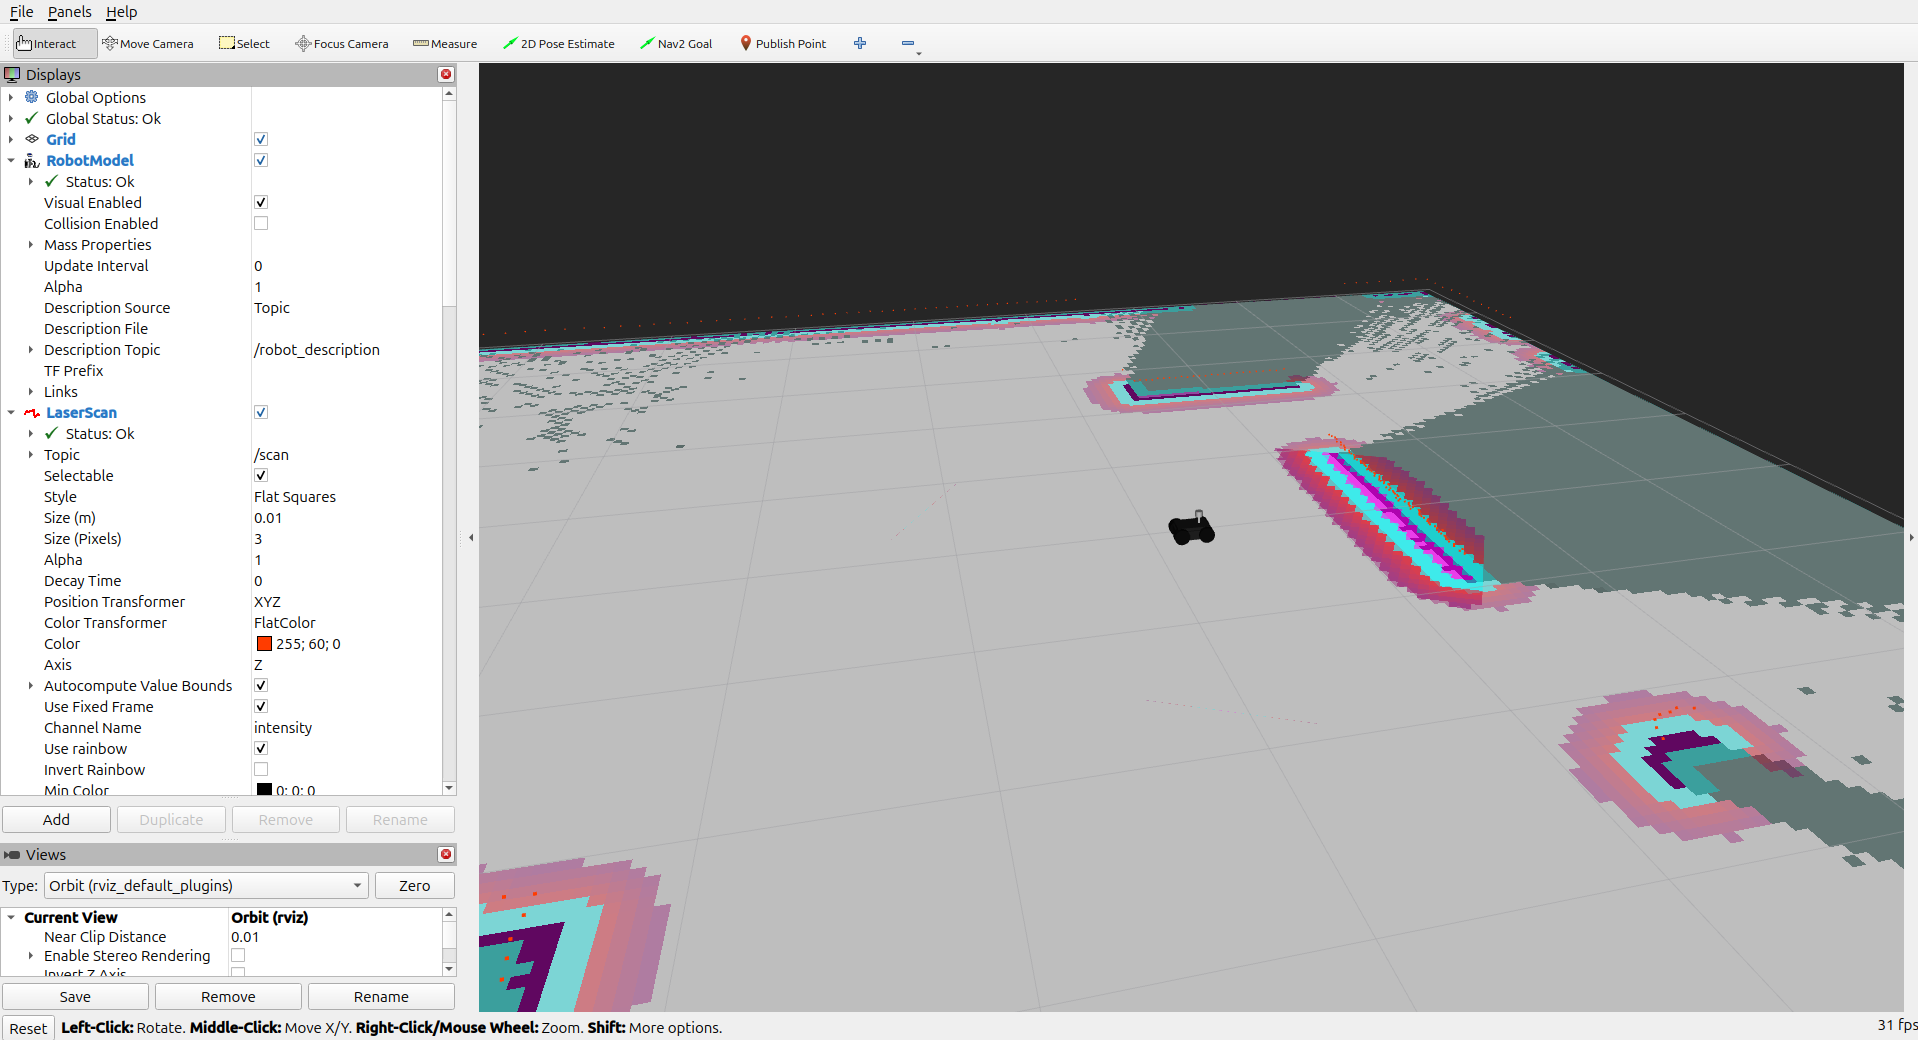
\includegraphics[height=5cm]{obrazky/model_rviz.png}
            \end{minipage}
            \hfill
            \begin{minipage}[t]{0.49\textwidth}
                \centering
                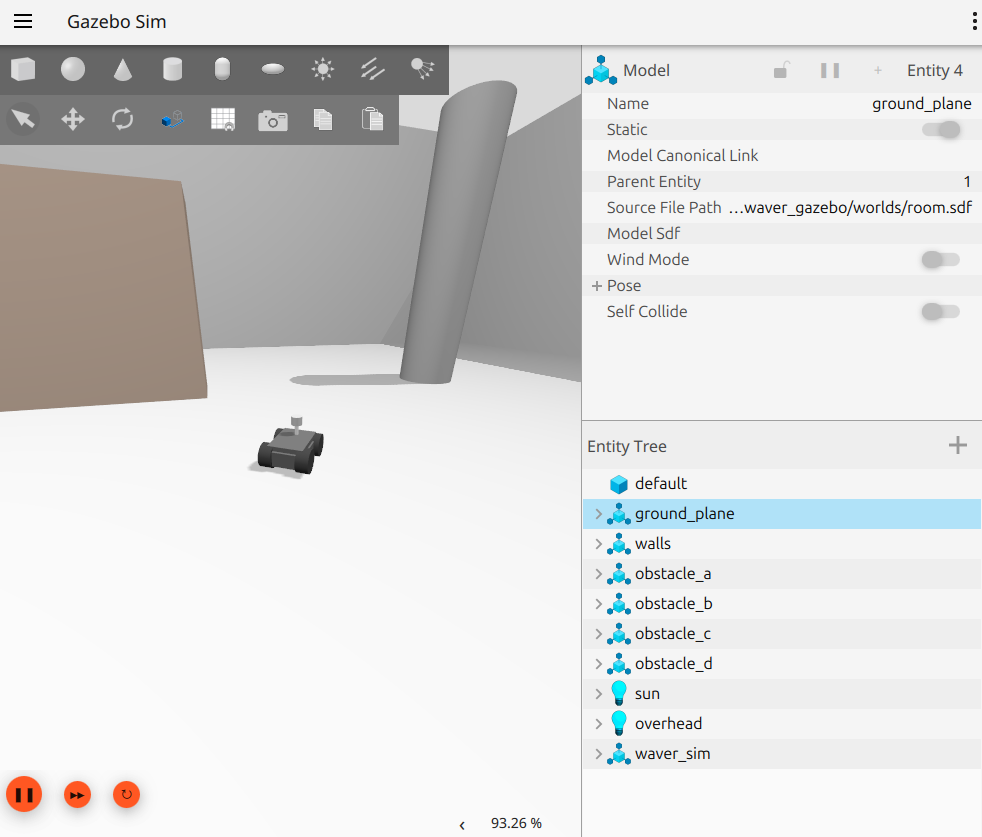
\includegraphics[height=5cm]{obrazky/gazebo.png}
            \end{minipage}
            \caption{Model Wave Rovera: vľavo RViz2, vpravo Gazebo Sim}
            \label{fig:model_rviz_waver}
        \end{figure}
      
        \section{Implementácia cez UGV Base General (\texorpdfstring{ESP32/HTTP}{ESP32--HTTP})}
        \label{sec:ugv_esp32_alternativa}
      
        Ešte pred vytvorením hlavnej implementácie bola overená aj referenčná konfigurácia založená na doske General Driver For Robots. Táto konfigurácia bola skúmaná ako alternatíva k priamemu riadeniu 
        motorov z Raspberry Pi, s cieľom overiť flexibilitu a možnosti 
        existujúceho firmvéru platformy.
      
        Riadenie v tejto konfigurácii vychádza z oficiálneho firmvéru UGV Base General\footnote{Oficiálny repozitár firmvéru: \url{https://github.com/waveshareteam/ugv_base_general}.}. Architektúra je rozdelená medzi dve samostatné výpočtové jednotky. Raspberry Pi plní úlohu nadradeného počítača, na ktorom beží ROS~2 a vyššie vrstvy riadenia, zatiaľ čo ESP32 zabezpečuje nízkoúrovňové ovládanie motorov a priamu komunikáciu s hardvérom podvozku.
      
        Komunikácia medzi oboma zariadeniami prebieha prostredníctvom HTTP požiadaviek s JSON obsahom. Raspberry Pi vďaka tomuto prístupu nemuselo byť fyzicky pripojené priamo k motorovému radiču ani pevne umiestnené na podvozku robota. Aj keď takýto spôsob integrácie nie je v prostredí ROS~2 taký bežný, prináša v tomto  prípade väčšiu flexibilitu a jednoduchosť.
      
        Na rozdiel od natívnej komunikácie v ROS~2, HTTP API firmvéru je striktne \emph{request--response}. Každý príkaz vyžaduje novú požiadavku a čakanie na odpoveď. Pre časovo kritické uzatvorené riadenie s vysokou frekvenciou a nízkym jitterom to nie je ideálne, lebo latencia závisí od zaťaženia ESP32, WiFi a parsovania JSON. Napriek tomu bol tento prístup vhodný na rýchle prototypovanie a overenie pohonu bez úprav firmvéru.
      
        \subsection{HTTP komunikácia s ESP32}
      
        Všeobecný tvar komunikácie je:
      
        \begin{verbatim}
        http://<ESP32_IP>/js?json=<URL_ENCODED_JSON>
        \end{verbatim}
      
        Každá správa obsahuje pole \texttt{T}, ktoré určuje typ operácie, a ďalšie parametre podľa požadovanej funkcie. Pri riadení pohybu sa používajú hodnoty ľavej a pravej strany pohonu. Príkladom je príkaz \texttt{\{"T":1,"L":0.3,"R":0.3\}}, ktorý nastaví obe strany na rovnakú doprednú rýchlosť. Hodnoty \texttt{L} a \texttt{R} sú normalizované v rozsahu od $-1$ do $1$.
      
        V prostredí ROS~2 túto komunikáciu zabezpečujú jednoduché mostové uzly, ktorých úlohou je preberať vstupy z tém alebo z klávesnice a prevádzať ich na HTTP požiadavky smerované na ESP32. Ide o preklad medzi internou komunikáciou ROS~2 a externým API. Každá zmena príkazu znamená aspoň jeden sieťový round-trip navyše oproti priamemu volaniu ovládača na I\textsuperscript{2}C z Raspberry Pi.
      
        Aj z tohto dôvodu bola táto architektúra použitá len na experimentálne účely 
        a hlavná implementácia bola realizovaná priamo na Raspberry Pi.
      
        \section{Architektúra hlavnej zostavy Wave Roveru}
        \label{sec:architektura-auticko}
      
        Zostava sa skladá z podvozku Wave Rover, Raspberry Pi~5, motorového HATu a pripojených senzorov. Z pohľadu architektúry je riešenie rozdelené do troch vrstiev. Prvú tvorí senzorická vrstva zahŕňajúca kameru, LiDAR a IMU. Druhú predstavuje riadiaca vrstva, v ktorej sa nachádza ovládanie motorov, korekčné algoritmy a autonómne režimy pohybu. Treťou je integračná vrstva, ktorá zabezpečuje spúšťanie systému, prepínanie režimov, webové rozhranie a prevádzkové služby.
      
        Rozdelenie systému na vrstvy oddeľuje zber a publikovanie senzorických dát od samotnej logiky pohybu. Samostatné uzly pre LiDAR alebo kameru sú úzko špecializované a ľahko vymeniteľné, zatiaľ čo DriveNode spolu s jednotlivými režimami (wander, jednoduchá bodová navigácia alebo sledovanie objektu) pracujú nad jednotným rozhraním.
      
        Takéto rozdelenie umožňuje oddeliť spracovanie senzorických dát 
        od riadiacej logiky a zároveň zjednodušuje rozšírenie systému. 
        Nové senzory alebo algoritmy je potom možné pridať ako samostatné uzly 
        bez zásahu do existujúcich častí systému.
      
        Alternatívne by sa dalo mať aj jeden veľký monolitický uzol, ktorý by naraz spracovával senzory, plánovanie aj riadenie motora. Také riešenie by však bolo postupom času ťažšie na testovanie, rozširovanie a rýchlo by v ňom vznikali problémy.
      
        \begin{figure}[H]
            \centering
            \begin{minipage}[t]{0.31\textwidth}
                \centering
                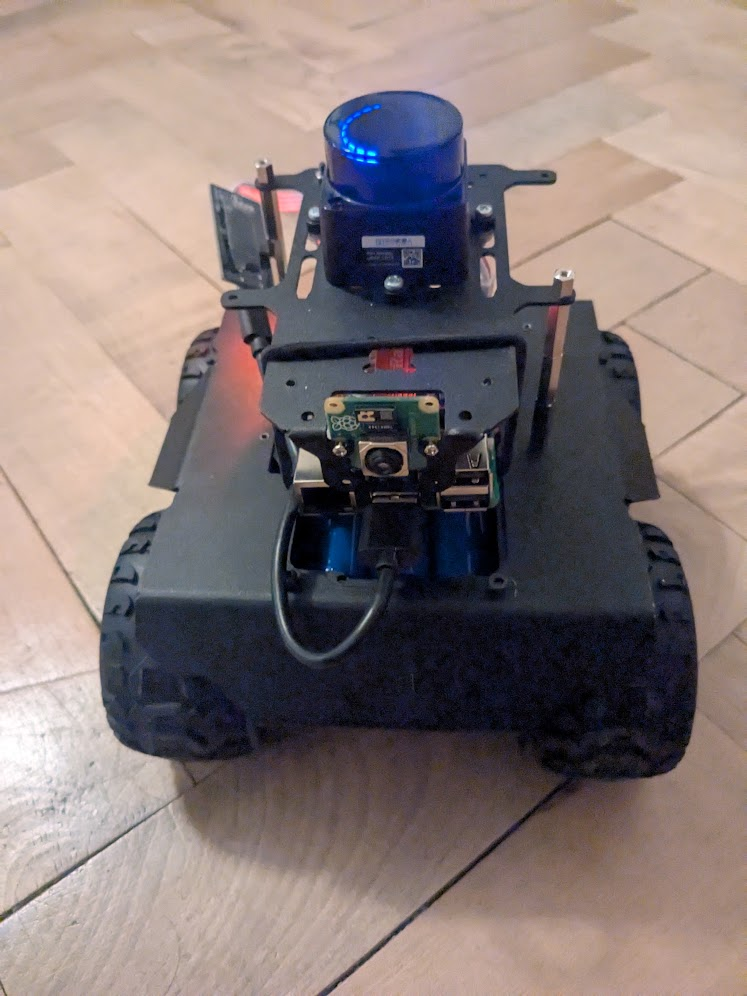
\includegraphics[width=\linewidth]{obrazky/rover_predok.jpg}\\[0.25em]
                {\small Pohľad spredu}
            \end{minipage}
            \hfill
            \begin{minipage}[t]{0.31\textwidth}
                \centering
                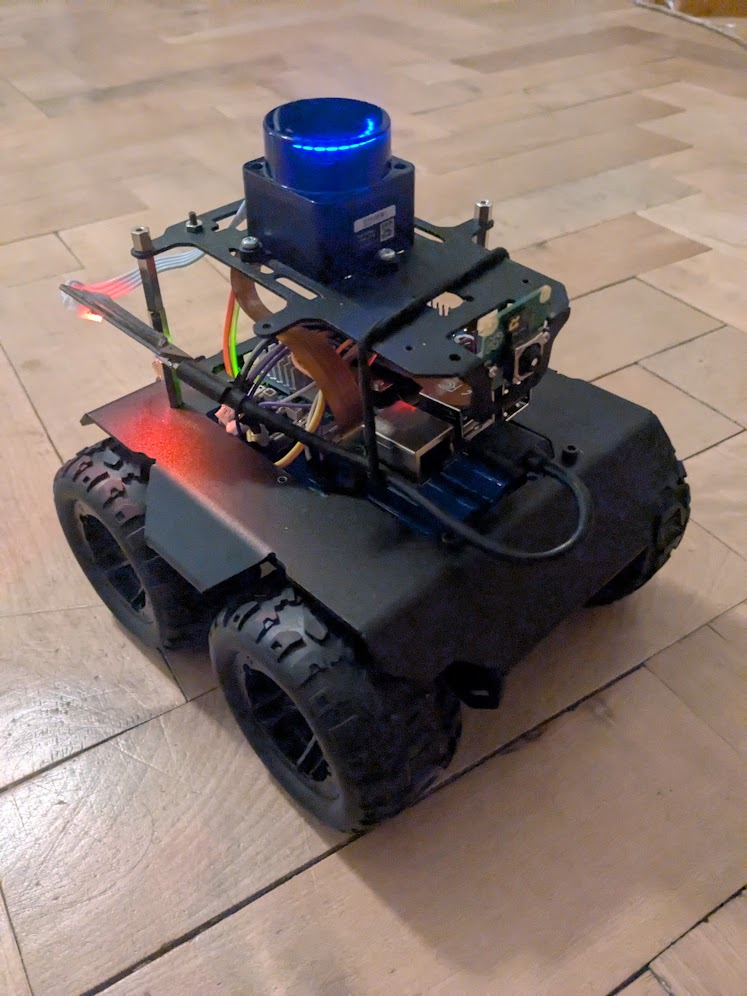
\includegraphics[width=\linewidth]{obrazky/rover_diag.jpg}\\[0.25em]
                {\small Šikmý pohľad}
            \end{minipage}
            \hfill
            \begin{minipage}[t]{0.31\textwidth}
                \centering
                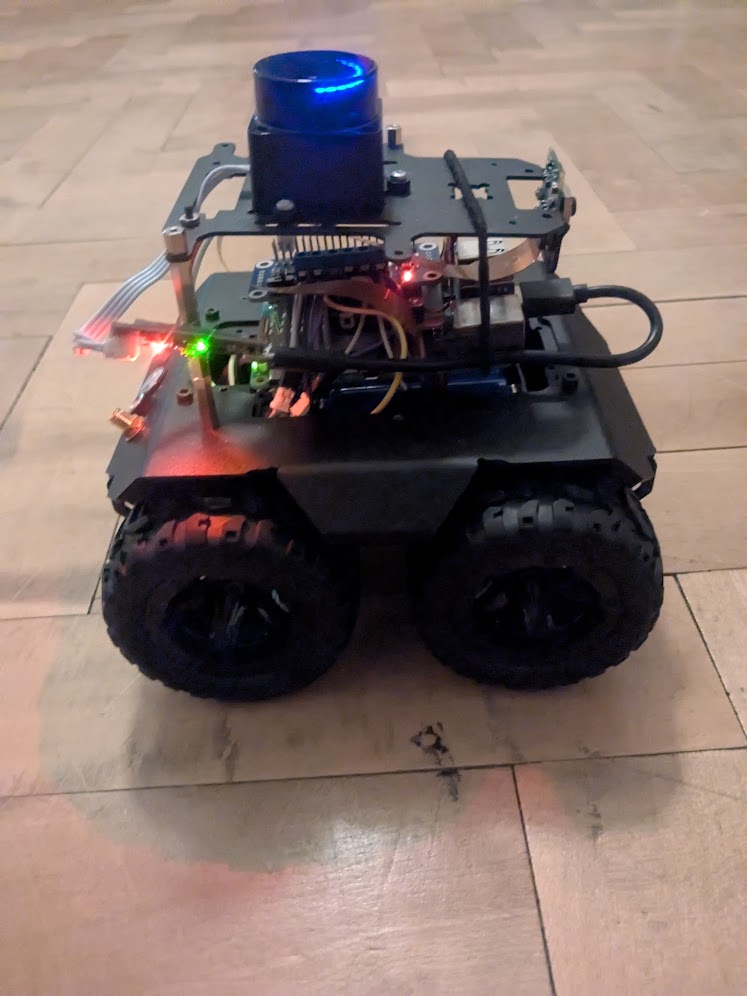
\includegraphics[width=\linewidth]{obrazky/rover_bok.jpg}\\[0.25em]
                {\small Pohľad zboku}
            \end{minipage}
            \caption[Wave Rover -- fyzická zostava]{Fyzická zostava platformy Wave Rover použitá pri hlavnej implementácii}
            \label{fig:wave-rover-fyzicka-zostava}
        \end{figure}
      
        \section{Manuálne ovládanie, motorový uzol a kamera}
        \label{sec:waverover-riadenie}
      
        Pred autonómnymi režimami a korekciou smeru je potrebné mať spoľahlivý základ: manuálne riadenie, jednotný výstup na motory a stabilný obraz z kamery. V tejto časti popisujem, ako tieto tri bloky spolu nadväzujú a aké ROS~2 rozhrania medzi nimi tečú.
      
        \subsection{Manuálne ovládanie a motorový uzol}
      
        Základným režimom práce robota je manuálne ovládanie. Na tento účel bol použitý štandardný uzol \texttt{teleop\_twist\_keyboard}, ktorý prevádza stlačenia kláves na správy typu \texttt{geometry\_msgs/msg/Twist}. Tieto správy predstavujú v ROS~2 bežný spôsob zadávania lineárnej a uhlovej rýchlosti.
      
        Samotný pohon robota zabezpečuje \texttt{DriveNode}, ktorý predstavuje jediný výstup smerom k motorom. Jeho úlohou je prijímať príkazy typu \texttt{Twist}, previesť ich na rýchlosti ľavej a pravej strany podvozku a následne generovať PWM signály pre motor HAT.
      
        Pri diferenciálnom podvozku sa otáčanie dosahuje rozdielom rýchlosti ľavej a pravej strany. Ak sa jedna strana zrýchli a druhá spomalí, vznikne moment, ktorý robota točí okolo zvislej osi. V teleop režime sa táto idea používa tak, že zložka \texttt{fb} (\emph{forward/back}) nastavuje spoločný pohon oboch strán (vpred alebo vzad), zatiaľ čo \texttt{tr} (\emph{turn}) pridáva k ľavej strane a uberá z pravej (alebo naopak), čím sa mení pomer krútiacich momentov a robot sa stáča.
      
        \begin{verbatim}
        target_l_ = std::clamp(-fb + tr, -1.0, 1.0);
        target_r_ = std::clamp(-fb - tr, -1.0, 1.0);
        \end{verbatim}
      
        Funkcia \texttt{std::clamp(..., -1.0, 1.0)} obmedzuje výsledné hodnoty do rozsahu, ktorý očakáva motorový ovládač. Bez tohto orezania by kombinácia zložiek pri prudkých vstupoch z klávesnice alebo webového rozhrania mohla prekročiť fyzikálne limity PWM signálu.
      
        Pre klasický model diferenciálneho podvozku~\cite{roboticsbook_diff_drive} sa pohyb robota rozkladá na lineárnu rýchlosť $v$ a uhlovú rýchlosť $\omega$. Tieto veličiny sa následne transformujú na rýchlosti ľavého a pravého kolesa podľa rozchodu kolies $b$ v štandardnom tvare unicycle modelu. Lineárna zložka ovplyvňuje obe kolesá rovnako, zatiaľ čo uhlová zložka spôsobuje rozdiel ich rýchlostí, čím vzniká rotácia robota.
      
        \begin{equation}
          v_L = v - \omega\,\frac{b}{2}, \qquad
          v_R = v + \omega\,\frac{b}{2}.
          \label{eq:diff-drive-unicycle}
        \end{equation}
      
        Korekcia jazdy v \path{drive_node.cpp} už nie je súčasťou samotného kinematického rozkladu a preto ju podrobnejšie rozoberiem v časti~\ref{sec:korekcia-smer-jazdy}.
      
        Webové rozhranie predstavuje paralelnú možnosť manuálneho ovládania. Pomocou \texttt{rosbridge} a knižnice \texttt{roslibjs} môže používateľ zadávať rovnaké príkazy z webového prehliadača.
      
        \subsection{Obraz z kamery pre teleop a vizuálnu korekciu}
        \label{sec:kamera-rpi5-ros2}
      
        Kamera plní v systéme dve hlavné úlohy. Prvou je poskytovanie živého obrazu pri diaľkovom ovládaní robota. Druhou je poskytovanie vstupu pre algoritmy vizuálnej korekcie pohybu. (Dodatočne neskôr slúži aj na detekciu a sledovanie objektu.)
      
        Po zapnutí modulu v launch konfigurácii je na Raspberry Pi spustený uzol \texttt{camera\_ros}. Uzol publikuje štandardné ROS témy s obrazom, kamerovou kalibráciou a komprimovaným streamom.
      
        \subsubsection{Živý náhľad v dialkovom webovom rozhraní}
        \label{sec:web-camera-webrtc}
      
        Pre náhľad z kamery v prehliadači sa neukázalo ako spolahlivé prenášať každý JPEG rámec cez \texttt{rosbridge}, pretože WebSocket nad TCP a serializácia správ zvyšovali oneskorenie aj záťaž systému. Preto je v \path{runtime_stack.launch.py} predvolene zapnuté \texttt{use\_webrtc\_camera:=true}, pričom obraz sa odoberá z ROS~2 a prenáša do prehliadača cez WebRTC.
      
        Ten istý obrazový tok je súčasne využívaný aj uzlom optického toku, ktorý prejdem v neskorších sekcíach.
      
        \section{Korekcia priameho smeru jazdy bez enkodérov}
        \label{sec:korekcia-smer-jazdy}
      
        Pri testovacích jazdách sa už pri bežnej jazde vpred rýchlo ukáže, že udržať smer nie je samozrejmosťou. Aj keď sú obom stranám motorov posielané rovnaké príkazy, robot sa začne mierne stáčať na jednu stranu. Dôvodov môže byť viac: rozdielne vlastnosti motorov, nerovnosti povrchu, odlišný valivý odpor kolies, drobná mechanická asymetria alebo krátkodobé prešmykovanie kolies.
      
        Pri platformách vybavených enkodérmi sa podobný problém zvyčajne rieši spätnou väzbou z otáčok kolies. V tomto prípade však boli použité motory bez enkodérov, takže nebolo možné priamo porovnávať skutočnú rýchlosť ľavej a pravej strany. Preto bolo nutné hľadať inú formu spätnej väzby, podľa ktorej by sa dalo určiť, či sa robot pri jazde vpred nechcene odchyľuje od smeru jazdy.
      
        V implementácii boli overované dve metódy. Prvá využíva IMU, konkrétne uhlovú rýchlosť okolo zvislej osi. Druhá vychádza z optického toku v obraze z kamery. Obe metódy sa snažia zachytiť ten istý jav, teda odchýlku od priameho smeru, ale vychádzajú z iného typu merania.
      
        \subsection{MPU-6050 na Arduino Nano a USB most}
        \label{sec:mpu6050-nano-usb}
      
        Pôvodne bol senzor MPU-6050 plánovaný na spoločnej I\textsuperscript{2}C zbernici spolu s motorovým HATom. Pri spustení sa však pri súčasnom riadení motorov a čítaní IMU objavovali nestability komunikácie, výpadky zariadení a nekorektné transakcie na zbernici. Keďže išlo o kritický bod celej architektúry, bolo zvolené hardvérové oddelenie IMU od tejto zbernice.
      
        Senzor MPU-6050 bol preto pripojený k samostatnému mikrokontroléru Arduino Nano, ktorý vykonáva lokálne čítanie dát cez vlastnú I\textsuperscript{2}C zbernicu. Firmvér na Nano po inicializácii senzora vykoná kalibráciu gyroskopu a periodicky odosiela dáta po USB. Na Raspberry Pi ich skript \path{imu_serial_fusion_bridge.py} parsuje a zostavuje z nich správy \texttt{sensor\_msgs/msg/Imu}.
      
        \subsection{Korekcia driftu podľa IMU}
      
        Cieľom nie je odhad absolútneho azimutu, ale zistenie, či sa podvozok pri jazde vpred neotáča. Pri rovnej jazde má byť $\omega_z$ z gyroskopu blízko nuly. Téma \rostopic{/imu} vzniká podľa časti~\ref{sec:mpu6050-nano-usb}. V moste sa pritom využíva aj komplementárny filter s akcelerometrom na stabilnejší odhad orientácie. Do regulátora v \texttt{DriveNode} však vstupuje predovšetkým priamo gyroskopická zložka $\omega_z$ .
      
        \subsubsection*{PID regulácia v motorovom uzle}
      
        Korekcia je implementovaná v \texttt{DriveNode}. Žiadaná hodnota je $\omega_{\mathrm{ref}} = 0$, takže chyba regulácie je $e_k = -\omega_{z,k}$. PID regulátor~\cite{astrom_murray_feedback} následne určuje korekciu ako kombináciu troch zložiek: okamžitej (proporcionálnej), kumulatívnej (integračnej) a predikčnej (derivačnej), pričom každá z nich ovplyvňuje správanie robota pri odchýlke od priamej jazdy.
      Pre potreby digitálnej implementácie v tomto systéme bol tento vzťah aproximovaný do diskrétneho tvaru:
        \begin{equation}
          u_k = K_p e_k + K_i \sum_{j=0}^{k} e_j\,\Delta t + K_d \frac{e_k - e_{k-1}}{\Delta t},
          \label{eq:pid-discrete}
        \end{equation}
      
        kde $u_k$ je výsledná korekcia aplikovaná diferenciálne na pohon – jedna strana sa zrýchľuje a druhá spomaľuje.
      
        Proporcionálna zložka reaguje okamžite na aktuálnu odchýlku, integračná odstraňuje dlhodobý drift a derivačná tlmí rýchle zmeny, čím stabilizuje reakciu systému. Koeficienty $K_p$, $K_i$, $K_d$ a obmedzenie integrátora sú nastaviteľné parametre uzla.
      
        V \path{drive_node.cpp} je pred aplikáciou PID na $\omega_z$ použitá mŕtva zóna a exponenciálne vyhladenie signálu. Podmienka \texttt{going\_straight} vypína korekciu pri zastavení, ostrých zatáčkach, veľkom rozdiele rýchlostí kolies alebo pri úmyselnom manévri, aby nezasahovala do zámerného riadenia.
      
        \begin{figure}[H]
          \centering
          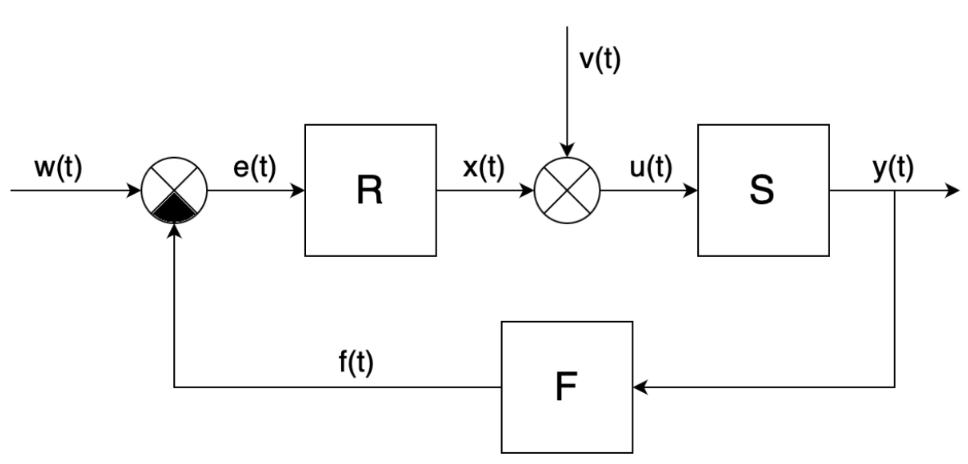
\includegraphics[width=0.6\linewidth]{obrazky/pid.png}
          \caption[Spätnoväzbová slučka regulácie]{Zovšeobecnená spätnoväzbová slučka: žiadaná hodnota $w(t)$, chyba $e(t)$, regulátor $R$, signál z regulátora $x(t)$, porucha $v(t)$, vstup do sústavy $u(t)$, sústava $S$, výstup $y(t)$, spätná väzba cez $F$.}
          \label{fig:pid-reg-loop}
        \end{figure}
      
        Použitý bol jednoduchý exponenciálny filter (EMA), ktorý obmedzuje šum a skoky:
        \begin{equation}
          y_k = \alpha x_k + (1-\alpha)\,y_{k-1}, \qquad \alpha \in (0,1),
          \label{eq:ema}
        \end{equation}
        pričom menšie $\alpha$ vedie k plynulejšej, ale pomalšej odozve. V implementácii sa používa na vyhladenie cieľových rýchlostí kolies (\texttt{smooth\_alpha}) aj na filtrovanie $\omega_z$ pred vstupom do PID (\texttt{imu\_yaw\_lowpass\_alpha}).
      
        Výstup PID regulátora sa následne aplikuje diferenciálne na pohon – z jednej strany sa odčíta a na druhej pripočíta, pričom výsledné hodnoty sa obmedzia do rozsahu \texttt{[-1, 1]} pomocou \texttt{std::clamp}, aby zostali v medziach motorového ovládača.
      
        \subsubsection*{Význam a využitie IMU korekcie}
      
        Metóda je vhodná pri slabom osvetlení a bez závislosti na textúre podlahy. Kvalita závisí od tlmenia šumu a biasu gyroskopu.
      
        \begin{figure}[H]
            \centering
            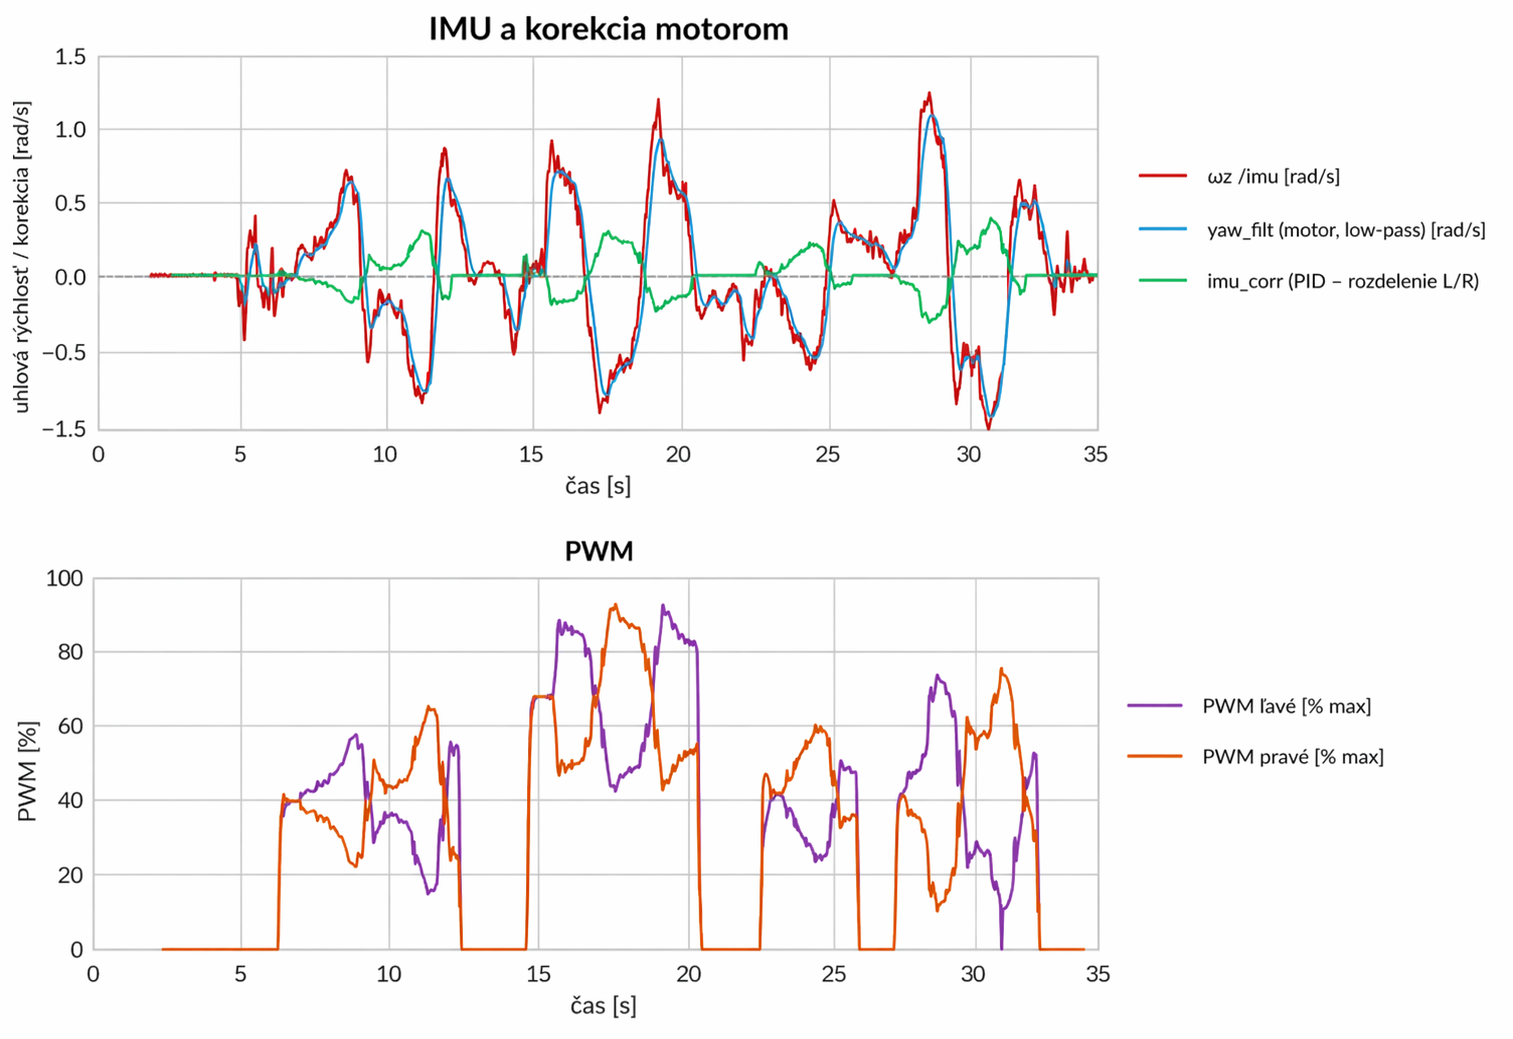
\includegraphics[width=0.9\linewidth]{obrazky/imu_graf.png}
            \caption[Priebeh IMU a korekcia pohonu]{Ukážka vzťahu medzi meranou uhlovou rýchlosťou a korekciou pohonu}
            \label{fig:imu-motor-correction}
        \end{figure}
      
        \subsection{Korekcia driftu podľa optického toku}
        \label{sec:korekcia-opticky-tok}
      
        Druhou skúšanou metódou bola korekcia podľa optického toku z kamery\footnote{OpenCV tutorial k optickému toku: \url{https://docs.opencv.org/3.4/d4/dee/tutorial_optical_flow.html}.}. Na rozdiel od IMU tu nejde o meranie rotácie priamo zo senzora, ale o pozorovanie toho, ako sa mení obraz pri pohybe robota podľa modelu Lucas--Kanade~\cite{lucas_kanade_1981}. Ak robot ide rovno dopredu a prostredie pred ním je približne statické, horizontálny posun obrazu by sa mal dlhodobo držať okolo nuly. Ak sa začne nechcene stáčať alebo uhýbať do strany, v obraze sa to prejaví ako postupný bočný posun sledovaných bodov. V implementácii sa z neho po priemerovaní a normalizácii vytvorí malá úprava \texttt{angular.z} v \texttt{Twist}, ktorá dopĺňa teleop rovnako ako pri IMU korekcii, ale z vizuálneho vstupu.
      
        \subsubsection*{Teoretický základ}
      
        Optický tok opisuje pohyb obrazových bodov medzi dvoma po sebe idúcimi snímkami. Zmeny polohy bodov umožňujú odhadnúť pohyb objektov alebo kamery v scéne.
      
        Metóda Lucas--Kanade vychádza z predpokladu konštantnosti jasu bodu medzi snímkami~\cite{lucas_kanade_1981}:
        $I(x,y,t) = I(x+\Delta x, y+\Delta y, t+\Delta t)$. Po linearizácii vznikne vzťah
        \begin{equation}
          I_x\,u + I_y\,v + I_t = 0,
        \end{equation}
        ktorý sa rieši pre rýchlosť pohybu $(u,v)$ v malom okolí bodu metódou najmenších štvorcov.
      
        V implementácii sa najprv vyberú stabilné body pomocou Shi--Tomasi detektora (\texttt{goodFeaturesToTrack})~\cite{shi_tomasi_1994}, ktorý preferuje rohy a výrazné hrany s vysokou zmenou intenzity v dvoch smeroch. Tieto body sa následne sledujú medzi snímkami pomocou \texttt{calcOpticalFlowPyrLK}.
      
        Výsledkom sú vektory posunu jednotlivých bodov, z ktorých sa pre riadenie využíva ich priemerná horizontálna zložka. Tá reprezentuje odchýlku robota od priamej jazdy a po normalizácii sa používa ako jemná korekcia uhlovej rýchlosti \texttt{angular.z}.
      
        \subsubsection*{Spracovanie v uzle \texttt{OpticalFlowNode}}

  Uzol priebežne odoberá obraz z kamery a sleduje aktuálny teleoperačný príkaz, ku ktorému môže podľa potreby pridať korekciu smeru.

  Každá snímka sa najprv dekóduje a prevedie do odtieňov sivej, keďže pre výpočet optického toku sú rozhodujúce zmeny jasu. Následne sa obraz zmenší, aby bol výpočet dostatočne rýchly.

  Na predchádzajúcej snímke sa vyberú body vhodné na sledovanie pomocou metódy Shi--Tomasi (\texttt{goodFeaturesToTrack})~\cite{shi_tomasi_1994}. Tieto body sa následne sledujú medzi snímkami pomocou metódy Lucas--Kanade (\texttt{calcOpticalFlowPyrLK})~\cite{lucas_kanade_1981}.

  Výpočet prebieha len v lokálnom okolí každého bodu, čo umožňuje efektívne spracovanie v reálnom čase.
      
        \begin{figure}[H]
          \centering
          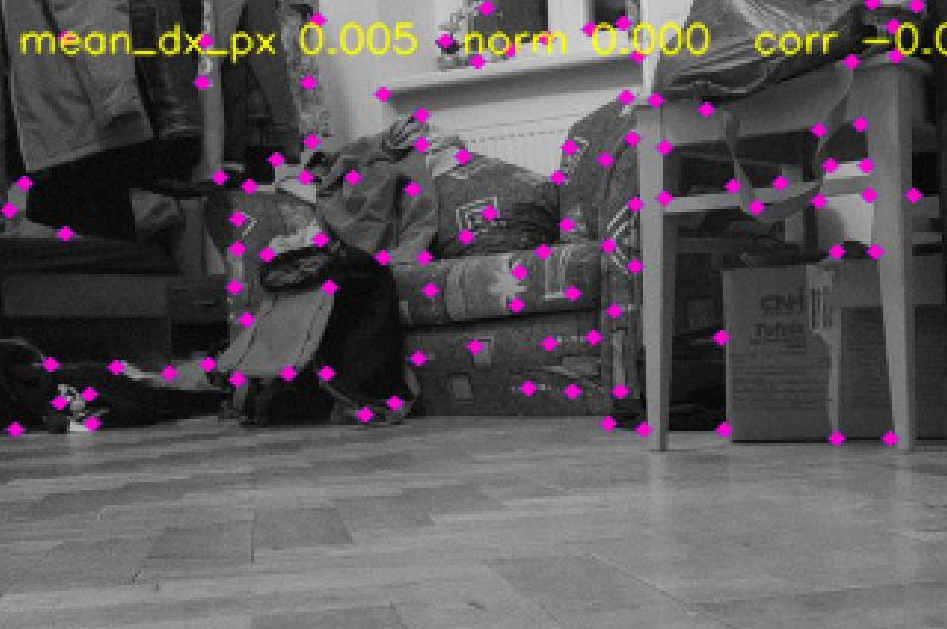
\includegraphics[width=0.7\linewidth]{obrazky/optical_flow_body.png}
          \caption[Sledované body optického toku]{Sledované body pri výpočte optického toku (ukážka z ladenia uzla)}
          \label{fig:optical-flow-tracked}
        \end{figure}
      
        \begin{verbatim}
        prev_pts = cv2.goodFeaturesToTrack(prev_gray, maxCorners=100,
                                          qualityLevel=0.01, minDistance=10)
        curr_pts, status, _ = cv2.calcOpticalFlowPyrLK(prev_gray, frame,
                                                        prev_pts, None)
        \end{verbatim}
      
        Zo všetkých úspešne sledovaných bodov sa počíta priemerný horizontálny posun. Ak sa napríklad väčšina bodov posúva v obraze doľava, znamená to, že robot má tendenciu uhýbať doprava. Znamienko a veľkosť priemernej hodnoty tak poskytujú jednoduchý odhad odchýlky od priameho smeru.
      
        Priemerovanie viacerých bodov má výhodu v tom, že výsledok je odolnejší voči chybným meraniam jednotlivých bodov. Ak sa niektorý bod stratí, zakryje alebo je vyhodnotený nepresne, ostatné body jeho vplyv zmiernia.
      
        Táto hodnota sa následne normalizuje podľa šírky obrazu, aby výsledok nebol závislý od použitého rozlíšenia. Po vynásobení nastaviteľným ziskom vznikne malá korekcia, ktorá sa pripočíta k zložke \texttt{angular.z}. Robot tak dostane povel na dorovnanie smeru jazdy.
      
        \begin{figure}[H]
          \centering
          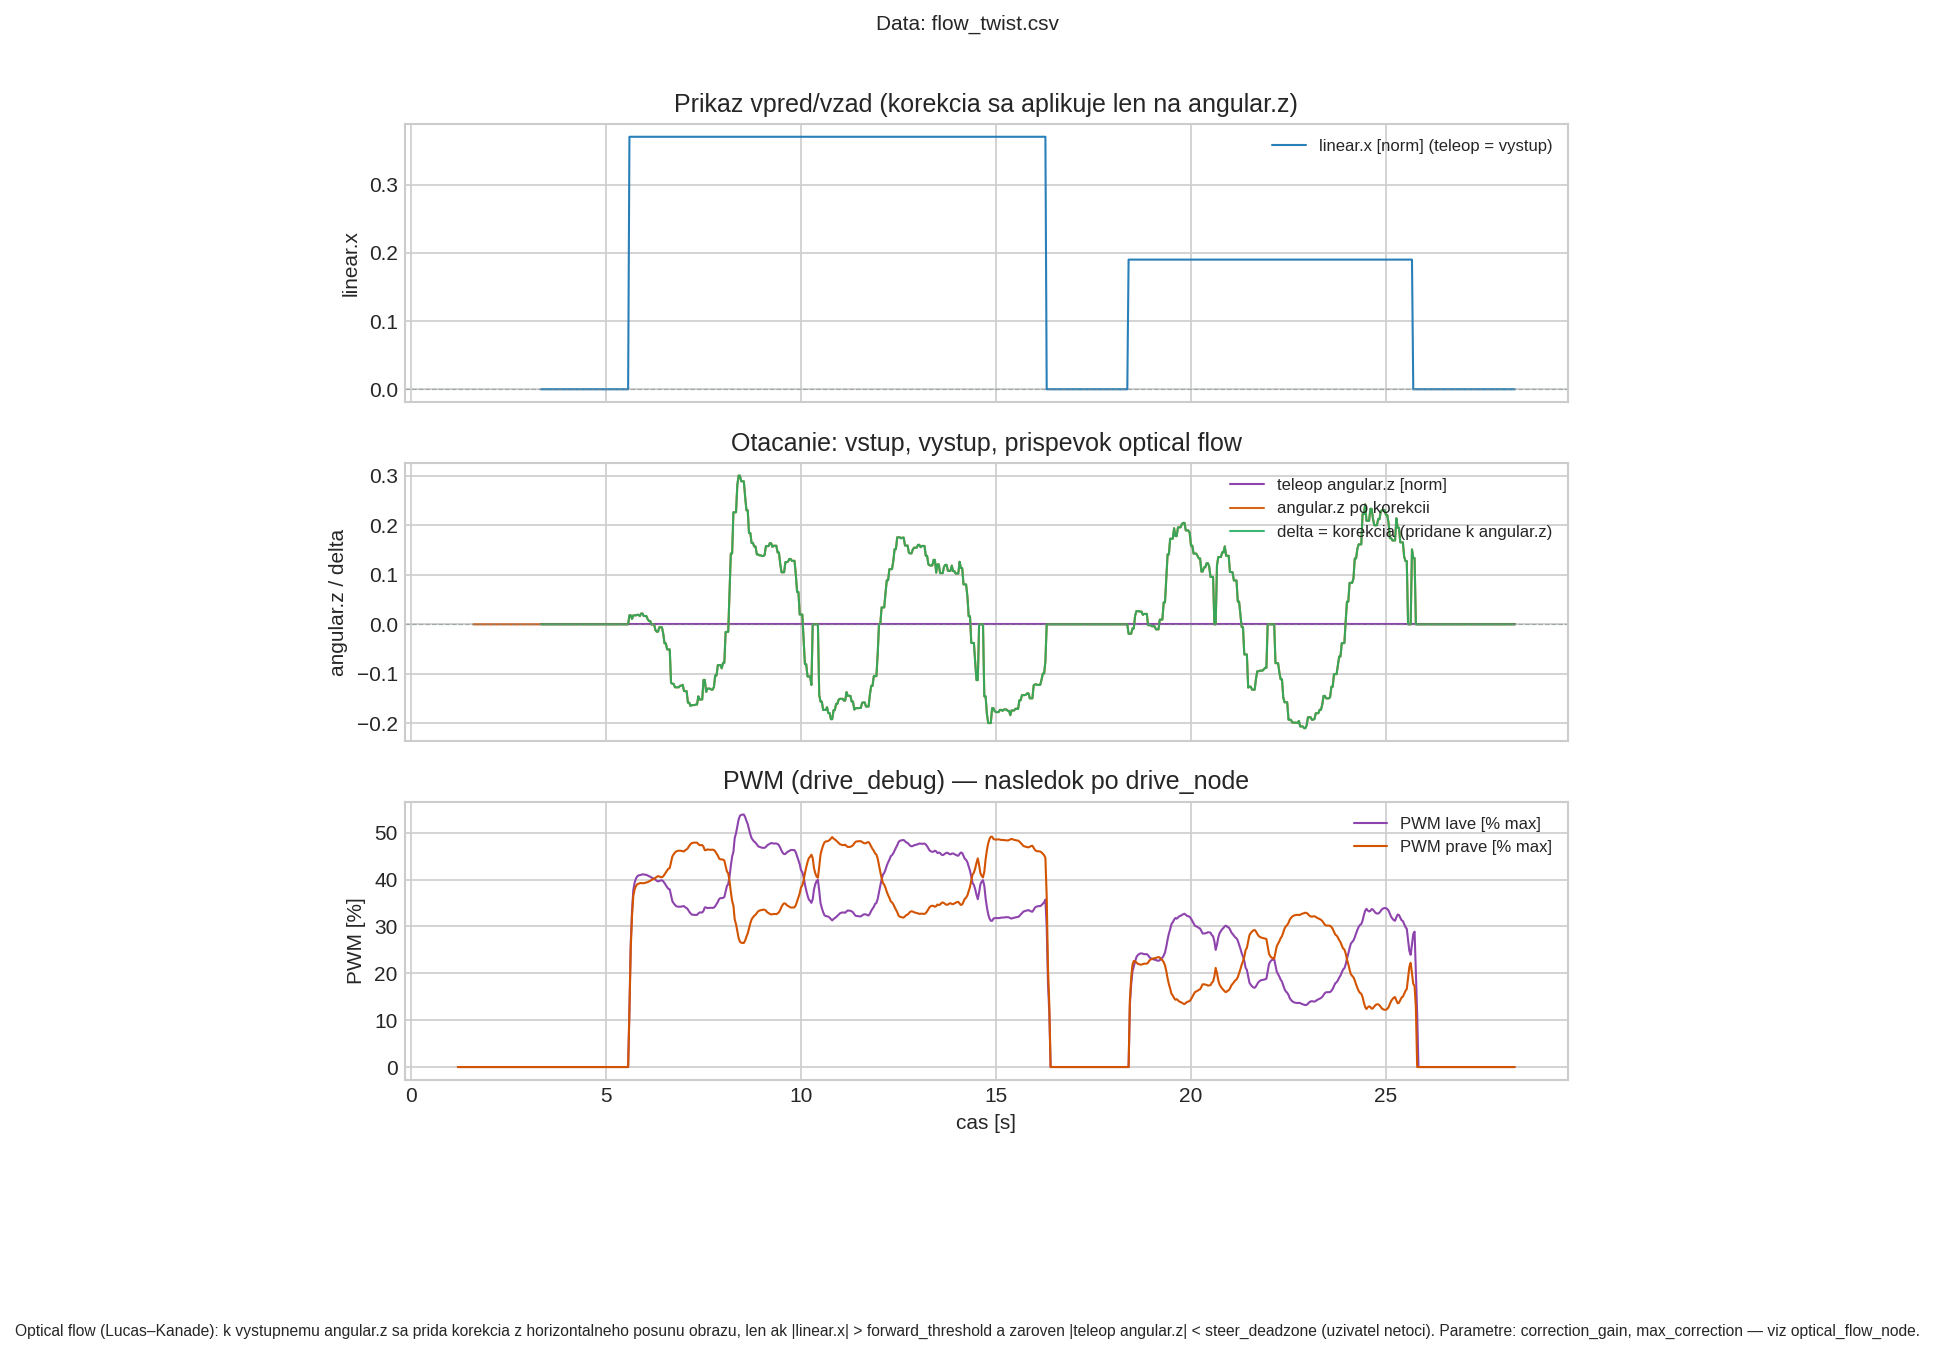
\includegraphics[width=0.88\linewidth]{obrazky/optical_flow_twist.png}
          \caption[Priebeh korekcie podľa optického toku]{Priebeh korekcie uhlovej zložky riadenia a súvisiacich signálov v čase (horný graf: \texttt{angular.z} a príspevok optického toku; dolný graf: PWM po spracovaní v \texttt{drive\_node})}
          \label{fig:optical-flow-correction}
        \end{figure}
      
      
        V grafoch tejto časti používam uhlovú rýchlosť okolo zvislej osi robota v jednotkách rad/s. Pri ideálne rovnej jazde má byť jej absolútna hodnota čo najmenšia.
      
        \begin{figure}[H]
          \centering
          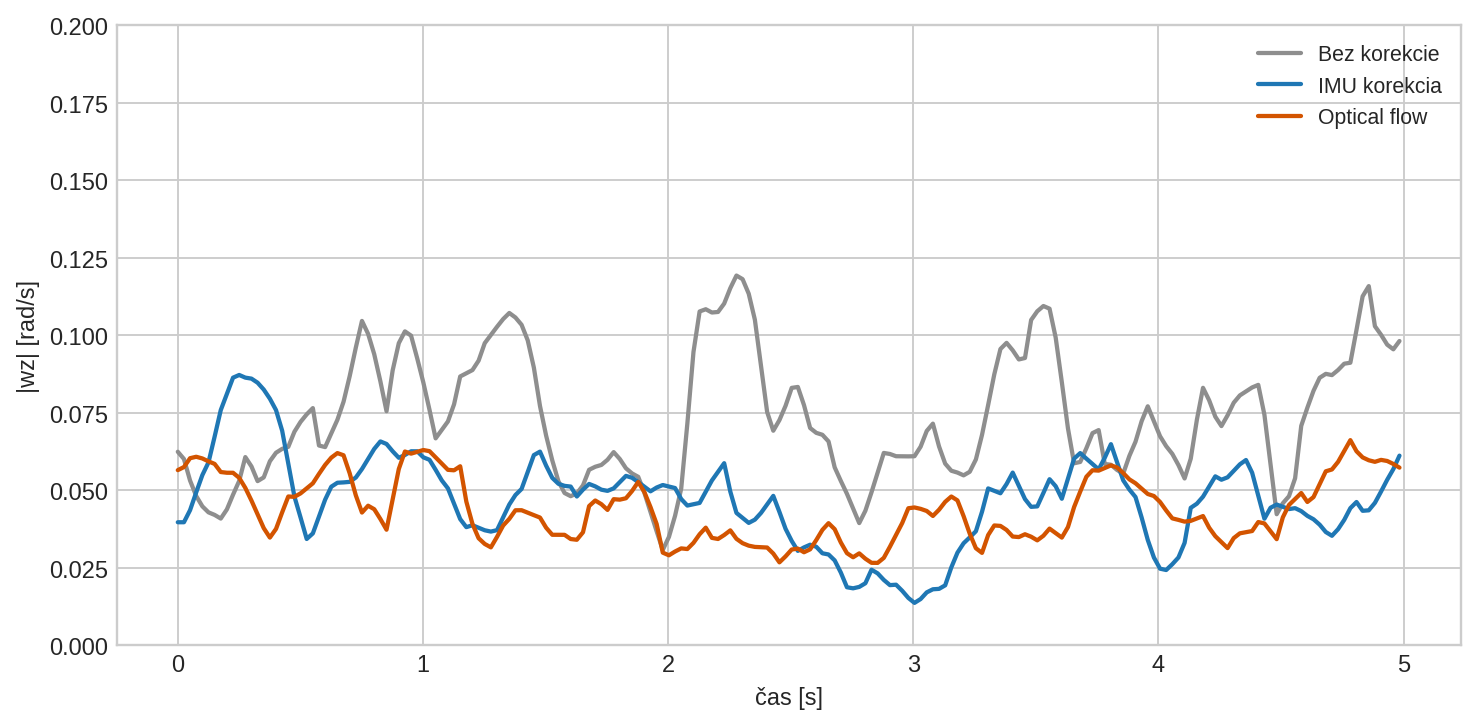
\includegraphics[width=0.8\linewidth]{obrazky/odchylka_porovnanie_3_rezimy_5s.png}
          \caption[Porovnanie odchýlky jazdy]{Porovnanie odchýlky jazdy počas 5-sekundového úseku pre tri režimy korekcie, pričom zobrazené priebehy predstavujú priemery z viacerých jazd.}
          \label{fig:odchylka-jazdy-porovnanie}
        \end{figure}
      
        \section{Autonómne blúdenie (wander)}
      
        Jedným z cieľov implementácie bolo doplniť platformu o autonómny režim pohybu. Na tento účel som implementoval režim \emph{wander} založený na reaktívnom vyhýbaní sa prekážkam podľa aktuálnych dát z LiDARu.
      
        Senzor LD19 je obsluhovaný driverom \texttt{ldlidar\_ros2}, ktorý publikuje laserový sken na tému \rostopic{/scan}. Namiesto spracovania celého skenu zložitým plánovačom je priestor okolo robota rozdelený na tri základné sektory: oblasť vpredu, oblasť vľavo a oblasť vpravo.
      
        Pre každý sektor sa z poľa \texttt{ranges} vyhodnocuje minimálna platná vzdialenosť. Neplatné merania alebo extrémne malé hodnoty sú ignorované.
      
        \begin{verbatim}
        def _sector_min(self, ranges, angle_min, angle_inc,
                        lo_deg, hi_deg, rotation_rad):
            best = math.inf
            for i, d in enumerate(ranges):
                if not math.isfinite(d) or d < 0.02:
                    continue
                ...
                if lo <= a_robot <= hi:
                    best = min(best, d)
            return best
        \end{verbatim}
      
        Takto získané tri hodnoty predstavujú zjednodušený model voľného priestoru v okolí robota a slúžia ako vstup pre rozhodovaciu logiku autonómneho režimu. 
      
        \begin{figure}[H]
            \centering
            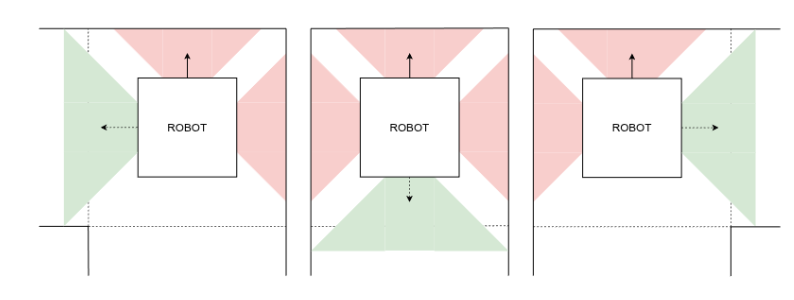
\includegraphics[width=0.75\textwidth]{obrazky/Wander_bloky.png}
            \caption[Bloková schéma režimu wander]{Rozhodovacia logika autonómneho blúdenia podľa miním v sektoroch}
            \label{fig:wander-block-diagram}
        \end{figure}
      
        \subsubsection{Stavový automat wanderu.}
      
        Riadenie je realizované ako jednoduchý stavový automat so stavmi jazdy vpred a otáčania. V predvolenom stave robot pokračuje dopredu konštantnou rýchlosťou \texttt{forward\_speed}, pokiaľ je priestor pred ním voľný a minimálna vzdialenosť v prednom sektore je väčšia než nastavený prah \texttt{threshold\_m}.
      
        Ak sa pred robotom objaví prekážka bližšie než zvolený limit, systém porovná voľný priestor v ľavom a pravom sektore. Následne vyberie vhodný smer otočenia. Ak je napríklad voľnejšia ľavá strana, robot sa otočí doľava. Ak sú obe strany podobne voľné, zvolí sa výhodnejší smer podľa väčšej vzdialenosti. V prípade, že sú blokované obe strany, vykoná sa otočenie o $180^\circ$.
      
        \begin{figure}[H]
          \centering
          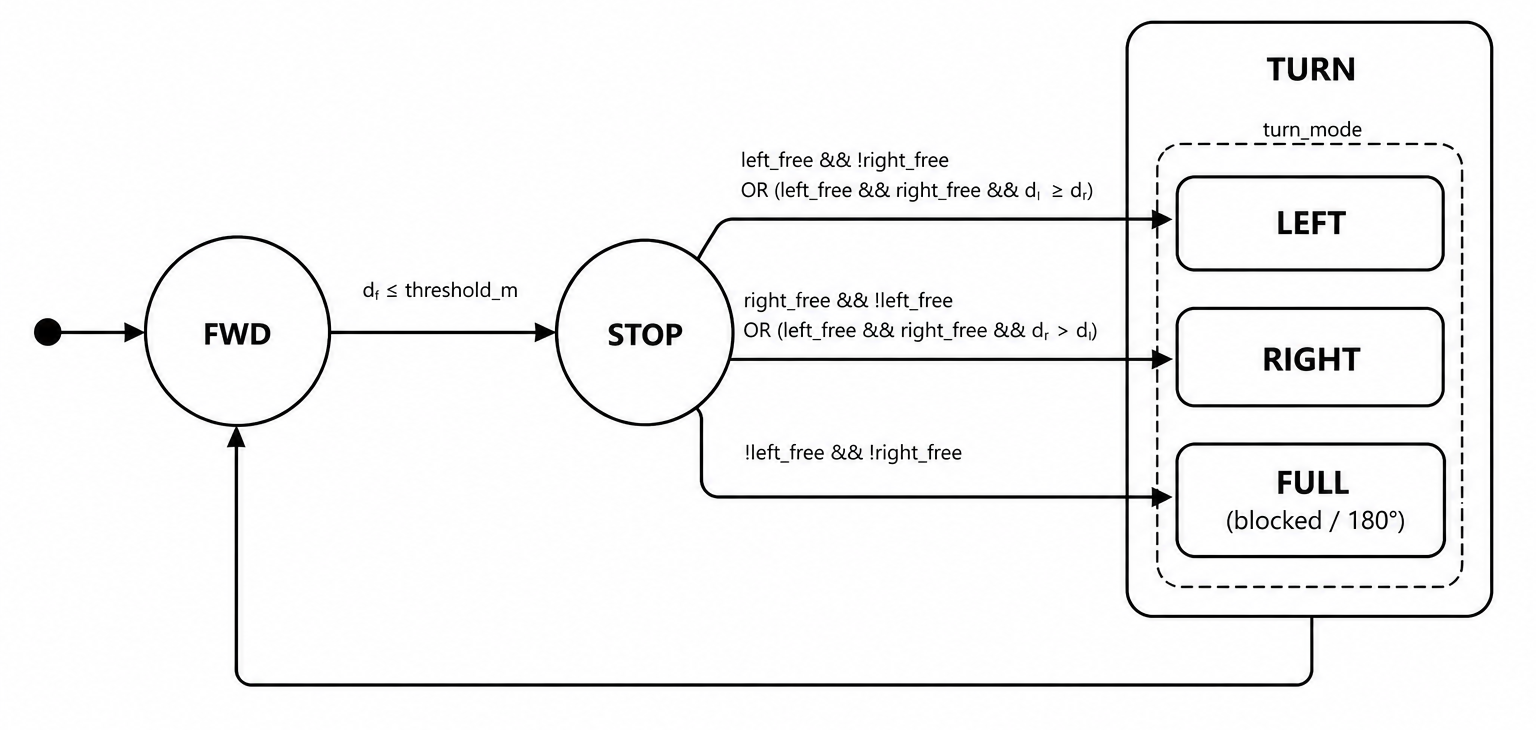
\includegraphics[width=0.7\textwidth]{obrazky/wander_automata.png}
          \caption[Stavový automat uzla wander]{Stavový automat uzla \texttt{lidar\_wander\_node} podľa implementácie v \path{lidar_wander.py}}
          \label{fig:wander-state-machine}
        \end{figure}
      
        Na obr.~\ref{fig:wander-rqt-scan} je ukážka behu režimu v nástroji \texttt{rqt}: laserový sken a súvisiace témy počas autonómneho blúdenia.
      
        \begin{figure}[H]
            \centering
            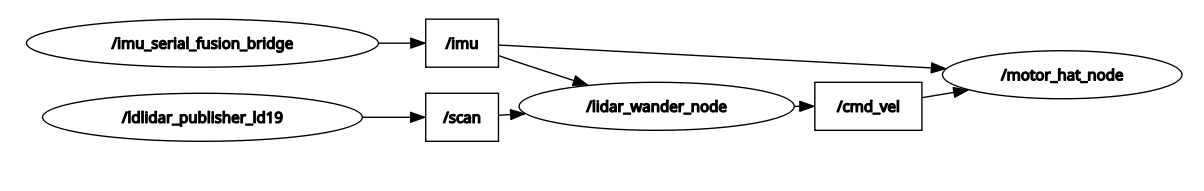
\includegraphics[width=0.75\textwidth]{obrazky/wander_rqt.png}
            \caption[Laserový sken pri režime wander]{Vizualizácia dát z LiDARu v nástroji \texttt{rqt} počas autonómneho bludenia}
            \label{fig:wander-rqt-scan}
        \end{figure}
      
        Počas otáčania robot generuje uhlovú rýchlosť okolo osi $z$. Odhad natočenia počas manévre sa v \path{lidar_wander.py} robí integráciou gyroskopickej zložky $\omega_z$ z IMU.
      
        \section{Mapovanie a jednoduchá bodová navigácia}
        \label{sec:mapovanie-simple-nav}
      
        Okrem reaktívneho wanderu som chcel ukázať aj prácu s mapou a cieľom v súradniciach \path{map}. Sekcia najprv stručne predstavuje 2D SLAM a distribuované spustenie náročnejších uzlov, potom jednoduchú bodovú navigáciu bez plného Nav2 stacku na reálnom podvozku.
      
        \subsubsection*{Mapovanie prostredia (SLAM)}
      
        Dôležitou súčasťou autonómneho pohybu Wave Roveru je schopnosť vytvárať mapu neznámeho prostredia a zároveň odhadovať vlastnú polohu v tejto mape. Táto úloha je známa ako \emph{SLAM} (\emph{Simultaneous Localization and Mapping}). Robot pri nej postupne získava merania zo senzorov, z ktorých buduje mapu okolia a súčasne spresňuje svoj odhad pozície.
      
        Na riešenie mapovania bol použitý balík \texttt{slam\_toolbox}, ktorý patrí medzi štandardné nástroje pre 2D SLAM v prostredí ROS~2. Zvolený bol pre jeho ľahkú integráciu s ostatnými časťami zostavy a priamu nadväznosť na navigačné úlohy.
      
        Balík pracuje predovšetkým s 2D LiDAR dátami a transformáciami medzi rámcami robota. Mapa je reprezentovaná \emph{occupancy grid}om, čo je pravidelná mriežka buniek, kde každej bunke zodpovedá odhad pravdepodobnosti obsadenia. Nové LiDAR skeny sa neukladajú len podľa odometrie, ale zarovnávajú sa voči už existujúcej mape, čím sa znižuje drift odhadu polohy.
      
        Súčasťou SLAM je aj \emph{uzatváranie slučiek}. Ak sa robot po čase vráti do už navštívenej oblasti, systém rozpozná známu časť prostredia a opraví nahromadenú chybu v trajektórii aj v mape. Vďaka tomu zostáva výsledná mapa konzistentnejšia aj pri dlhšom pohybe.
      
        \begin{figure}[H]
            \centering
            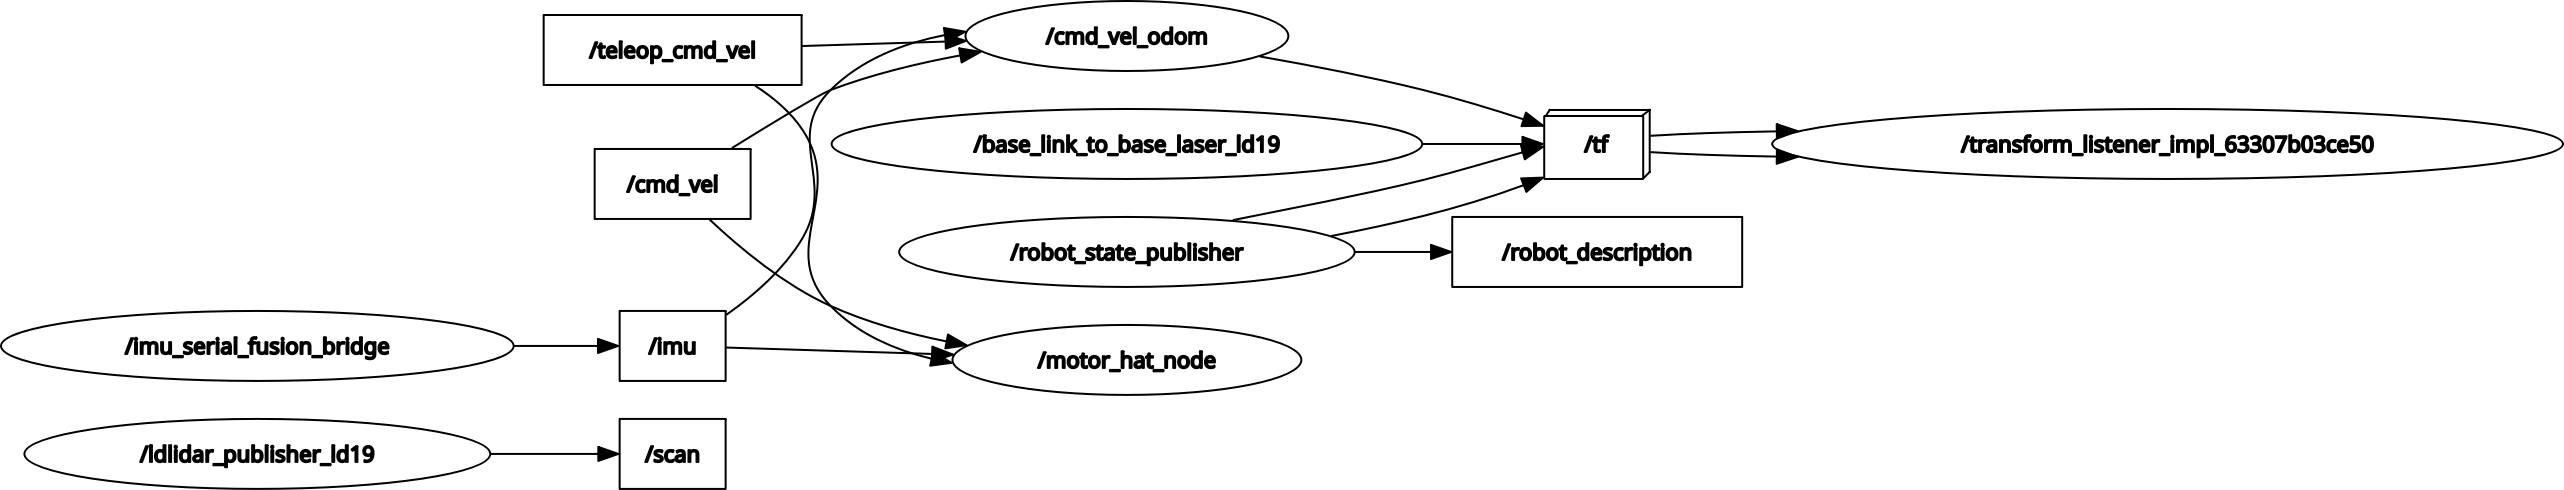
\includegraphics[width=0.8\linewidth]{obrazky/manual+slam_rqt.png}
            \caption[Graf uzlov pri manuálnom ovládaní a SLAM]{Prepojenie uzlov pri manuálnom režime a súčasne spustenom mapovaní}
            \label{fig:manual-slam-rqt-graph}
        \end{figure}
      
        \subsubsection*{Distribuované nasadenie}
        \label{sec:distrib-slam-rviz}
      
        Výpočtovo náročnejšie časti systému, najmä SLAM a plynulá vizualizácia v RViz, výrazne zaťažovali Raspberry Pi, čo sa prejavovalo na stabilite ostatných procesov. Z tohto dôvodu som tieto komponenty spúšťal na výkonnejšom externom počítači.
      
        Na Raspberry Pi zostáva \emph{runtime stack} zabalený v \path{runtime_stack.launch.py}. Pri zapnutí mapovania s parametrom \texttt{use\_offboard\_slam:=true} sa uzol \texttt{slam\_toolbox} nespúšťa na Raspberry Pi, ale beží na externom počítači pomocou launch súboru \path{slam_remote_pc.launch.py}. Na tomto počítači je zároveň spustený aj RViz, ktorý slúži na vizualizáciu mapy a aktuálneho stavu lokalizácie.
      
      
        \subsection*{Jednoduchá navigácia}
      
        V systéme je okrem režimu \emph{wander} implementovaný aj jednoduchý navigačný režim \emph{simple nav}, aby bolo možné aspoň sčasti ukázať 
        základné princípy riadenia bez komplexného Nav2 stacku.
      
        Cieľ sa zadáva v RViz pomocou nástroja \emph{2D Goal Pose} a prichádza ako správa \texttt{geometry\_msgs/msg/PoseStamped} na tému \rostopic{/goal_pose}. Poloha cieľa aj aktuálna poloha robota sa získavajú z transformácie \texttt{map} $\rightarrow$ \texttt{base\_link} cez SLAM.
      
        Po prijatí cieľa sa robot najprv otočí smerom k nemu a následne sa k nemu pohybuje priamo dopredu. Rýchlosti sa posielajú ako \texttt{geometry\_msgs/msg/Twist} na \rostopic{/cmd_vel}.
      
        V simulácii bol použitý plnohodnotný stack Nav2, ktorý obsahuje globálne aj lokálne plánovanie. V reálnom nasadení sa však ukázalo, že priame riadenie cez Nav2 a generované rýchlosti nebolo dostatočne stabilné. Preto bola implementovaná primitívnejšia verzia, ktorá rieši iba presun medzi bodmi bez komplexného plánovania.
      
        \section{Sledovanie farebnej lopty}
        \label{sec:ball-follow-section}
      
        V tejto časti opisujem sledovanie jednofarebného objektu (v testoch pomaranč) pomocou kamery a následné priblíženie robota. Z obrazu sa vždy vyberá len horizontálna odchýlka cieľa od stredu záberu a veľkosť jeho projekcie v pixeloch. Na základe týchto dvoch hodnôt regulátor generuje príkaz \texttt{Twist}, ktorý sa publikuje na tému \rostopic{/cmd_vel} podobne, ako to bolo u korekcii jazdy.
      
        Postup detekcie vychádza z farebnej segmentácie v HSV, ošetrenia binárnej masky a extrakcie kontúr. Konkrétne funkcie a operácie pri jednotlivých krokoch odkazujem na príslušné časti dokumentácie OpenCV nižšie. V implementácii sa používa vlastný výber kandidáta z kontúr. Ako východiskový nápad poslúžil verejný ROS~2 balík Josha Newansa\footnote{Repozitár \texttt{ball\_tracker}: \url{https://github.com/joshnewans/ball_tracker}.}, no v navrhnutom riešení je nad ním postavená vlastná riadiaca vrstva s rozhodovacou logikou sledovania a spôsobom spúšťania.
      
        \subsubsection*{Tri vrstvy Architektúry}
      
        \begin{itemize}
          \item \path{detector.py} --- obsahuje triedu \texttt{OrangeDetector}, ktorá vracia štruktúru \texttt{Detection} (\texttt{x\_err}, \texttt{radius\_px}, \texttt{confidence}).
          \item \path{controller.py} --- trieda \texttt{BallController}, ktorá spracuje detekciu cez \texttt{update(det, has\_frame)} a vráti \texttt{Twist} spolu so stavom.
          \item \path{action_node.py} --- \texttt{BallFollowerNode}, ktorý zabezpečuje príjem obrazu, publikovanie dôvery v správnu detekciu, debug obraz a akčný server typu \texttt{FollowBall}.
        \end{itemize}
      
        \subsubsection*{Detekcia v \texttt{OrangeDetector}}
      
        Detekcia začína funkciou \texttt{\_make\_mask}. Najprv sa vstupný obraz zmenší na polovicu, aby sa znížila výpočtová náročnosť, pričom sa stále zachová dostatok informácie na spoľahlivú detekciu objektu.
      
        Následne sa obraz prevedie z farebného priestoru BGR do HSV, ktorý je pre farebnú segmentáciu vhodnejší, pretože oddelí informáciu o farbe od jasu. Na základe nastavených intervalov pre oranžovú farbu (\texttt{orange\_h\_min/max}, \texttt{s\_*}, \texttt{v\_*}) sa pomocou funkcie \texttt{cv2.inRange}~\cite{opencv_inrange_tutorial} vytvorí binárna maska, kde sú pixely patriace lopte biele a zvyšok čierny.
      
        Takto vzniknutá maska však obsahuje aj drobné šumy a rušenie, preto sa ďalej čistí morfologickými operáciami (\textbf{opening} \texttt{MORPH\_OPEN}, \textbf{closing} \texttt{MORPH\_CLOSE}) podľa \cite{opencv_morphology_tutorial}: opening je zložením erozie a dilatácie a odstraňuje drobné artefakty, closing je zložením dilatácie a erozie a vypĺňa malé dierky v oblasti objektu. V implementácii najprv nasleduje opening, potom closing.
      
        Z výslednej masky sa následne extrahujú kontúry pomocou \texttt{findContours(..., RETR\_EXTERNAL)}~\cite{opencv_contours_tutorial}, pričom sa berú len vonkajšie obrysy objektov. Veľmi malé kontúry sa zahadzujú, pretože zvyčajne znamenajú šum alebo odrazy.
      
        Pre každú zostávajúcu kontúru sa vyhodnocuje, či ide skutočne o guľu podľa rôznych vlastností. Na vyhodnotenie kandidátnych kontúr sa v implementácii používa vlastná skórovacia heuristika. Z geometrických vlastností kontúry sa zostaví veličina spoľahlivosti:
      
        \[
          \texttt{conf} = \mathrm{clip}\bigl(0{,}40\,c + 0{,}35\,s + 0{,}15\,a + 0{,}10\,\mathrm{clip}(f,0,1)\bigr),
        \]
      
        kde $c$ predstavuje kruhovitosť, $s$ soliditu, $f$ vyplnenie kruhu a $a$ normalizovanú plochu vzhľadom na veľkosť masky. Ak je výsledná hodnota menšia než prah \texttt{min\_confidence}, kontúra sa ignoruje. Z platných kandidátov sa následne vyberie tá s najvyššou spoľahlivosťou.
      
        Pozícia lopty sa určuje až na pôvodnom rozlíšení obrazu. Zo stredu detegovaného kruhu sa v implementácii počíta normalizovaná horizontálna odchýlka od stredu, kde $w$ je šírka obrazu:
      
        \[
          \texttt{x\_err} = \frac{c_x - w/2}{w/2},
        \]
        
      
  Keďže detekcia môže občas preskočiť na iný objekt alebo šum, systém kontroluje, či sa poloha stredu medzi snímkami príliš nezmenila. Ak je skok väčší než povolený limit, detekcia sa zahodí a označí sa ako miss. Ak sa takáto situácia opakuje dlhšie, než je nastavený čas \texttt{jump\_reset\_sec}, história sledovania sa resetuje, aby sa systém znovu stabilizoval.
      
  Pre ladenie som generoval vizuálny výstup, ktorý zobrazuje masku prekrytú na pôvodnom obraze, stred obrazu, detegovaný kruh a aktuálnu pozíciu lopty. Dopĺňajú sa aj hodnoty polomeru, odchýlky \texttt{x\_err} a spoľahlivosti \texttt{conf}.
      
        \begin{figure}[htbp]
            \centering
            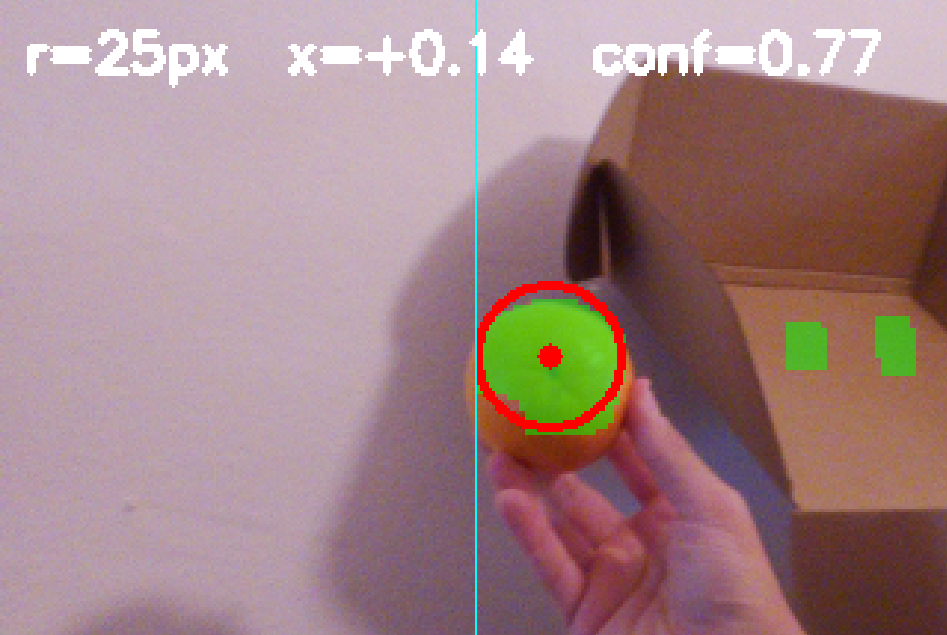
\includegraphics[width=0.65\linewidth]{obrazky/pomaranc.png}
            \caption[Sledovanie objektu: debug obraz]{Debug v \texttt{rqt\_image\_view} na \rostopic{/ball_follower/debug_image/compressed}: maska, polomer a horizontálna odchýlka.}
            \label{fig:ball-follow-debug}
        \end{figure}
      
        \subsubsection*{Rozhodovacia logika \texttt{BallController}}
      
        Riadenie sledovania nie je v kóde zapísané ako tabuľka prechodov klasického stavového automatu, ale ako priradenie režimu v každom volaní \texttt{update()}: z aktuálneho vstupu (snímka, detekcia, polomer, čas od poslednej detekcie) sa vypočíta príkaz \texttt{Twist} a súčasne sa označí jedna z hodnôt výčtu \texttt{State} (\texttt{SEARCH}, \texttt{TRACK}, \texttt{APPROACH}, \texttt{COAST}, \texttt{STOP}).
      
        Ak nie je k dispozícii obraz, výstup je bezpečná zástava a režim \texttt{SEARCH}. Pri krátkodobej strate detekcie sa použije \texttt{COAST} s poslednou zapamätanou doprednou rýchlosťou. Ak je objekt v zábere dostatočne veľký, aktivuje sa \texttt{STOP}.
      
        Inak robot cieľ sleduje v režime \texttt{TRACK}; pri približovaní v pásme pred zastavením sa rýchlosť a zatáčanie zmierňujú (\texttt{APPROACH}) podľa \texttt{stop\_radius\_px} a \texttt{brake\_band\_px}. Obr.~\ref{fig:ballfollow-fsm} zobrazuje rovnakú logiku vo forme toku rozhodnutí pre jedno volanie \texttt{update()}.
      
        \begin{figure}[H]
            \centering
            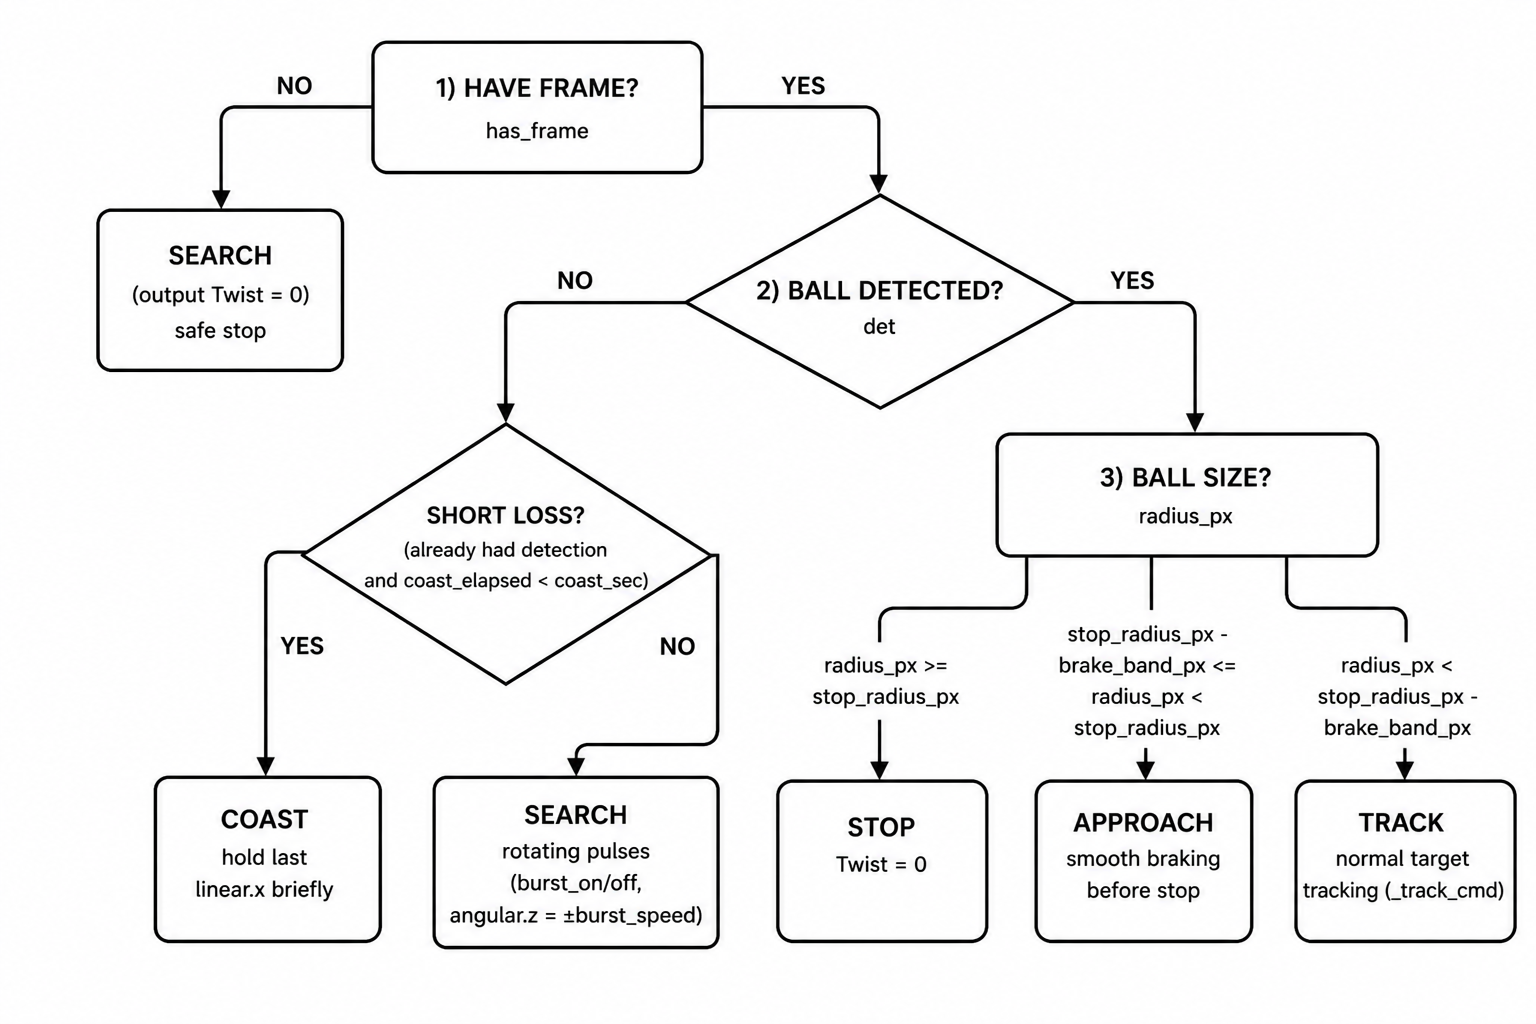
\includegraphics[width=0.85\linewidth]{obrazky/ballfollow_automat.png}
            \caption{Rozhodovací diagram režimov sledovania lopty (\texttt{BallController}, metóda \texttt{update()}).}
            \label{fig:ballfollow-fsm}
        \end{figure}

              Vplyv vzdialenosti objektu sa zohľadňuje škálovaním podľa jeho polomeru, čím sa zvyšuje citlivosť riadenia pri bližšom objekte. Výsledný príkaz Twist je následne obmedzený na bezpečný rozsah a vyhladený pomocou EMA filtra.
      
        \begin{figure}[htbp]
            \centering
            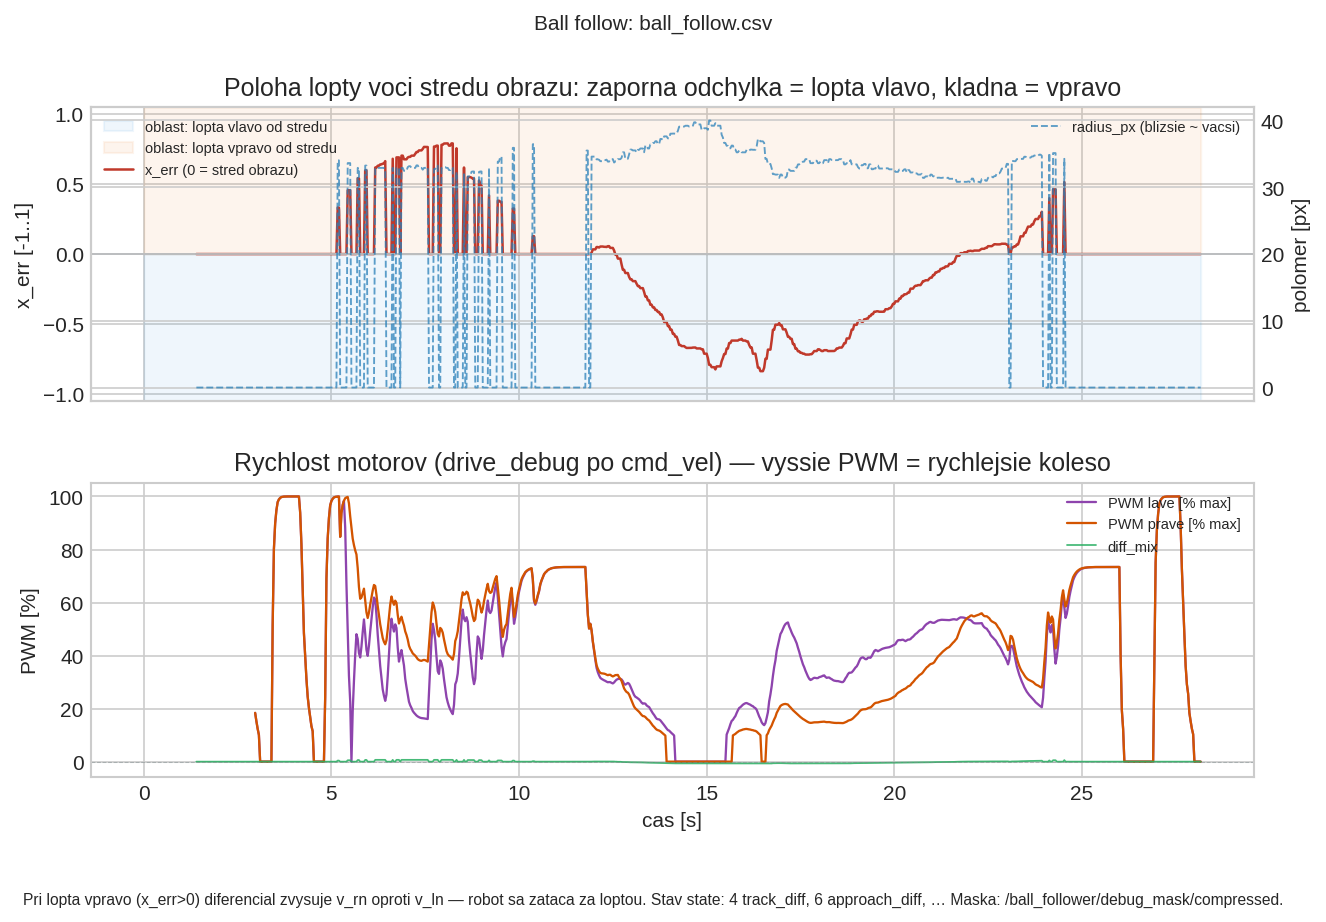
\includegraphics[width=0.88\linewidth]{obrazky/ball_follow_graf.png}
            \caption[Sledovanie objektu: priebeh rýchlostí]{Priebeh lineárnej a uhlovej rýchlosti počas sledovania objektu.}
            \label{fig:ball-follow-graph}
        \end{figure}
      
        \subsubsection*{Behaviorálny strom ako orchestrátor}
      
        \texttt{BallController} rieši lokálnu rozhodovaciu logiku sledovania objektu, napríklad 
        reakciu na stratu cieľa, zatiaľ čo behaviorálny strom riadi celkové 
        správanie robota na vyššej úrovni.
      
        Vyššiu logiku úlohy zabezpečuje uzol \path{bt_runner.py} využívajúci knižnicu \texttt{py\_trees}~\cite{py_trees_docs}. Behaviorálny strom (Obr.~\ref{fig:ball-follow-bt-diagram}) organizuje celý priebeh sledovania do troch na seba nadväzujúcich fáz: \textbf{FindBall}, \textbf{FollowBall} a \textbf{Celebrate}. Jednotlivé kroky opakovane využívajú ten istý akčný server \texttt{follow\_ball}, ale s rôznymi parametrami cieľa.
      
        \begin{figure}[H]
          \centering
          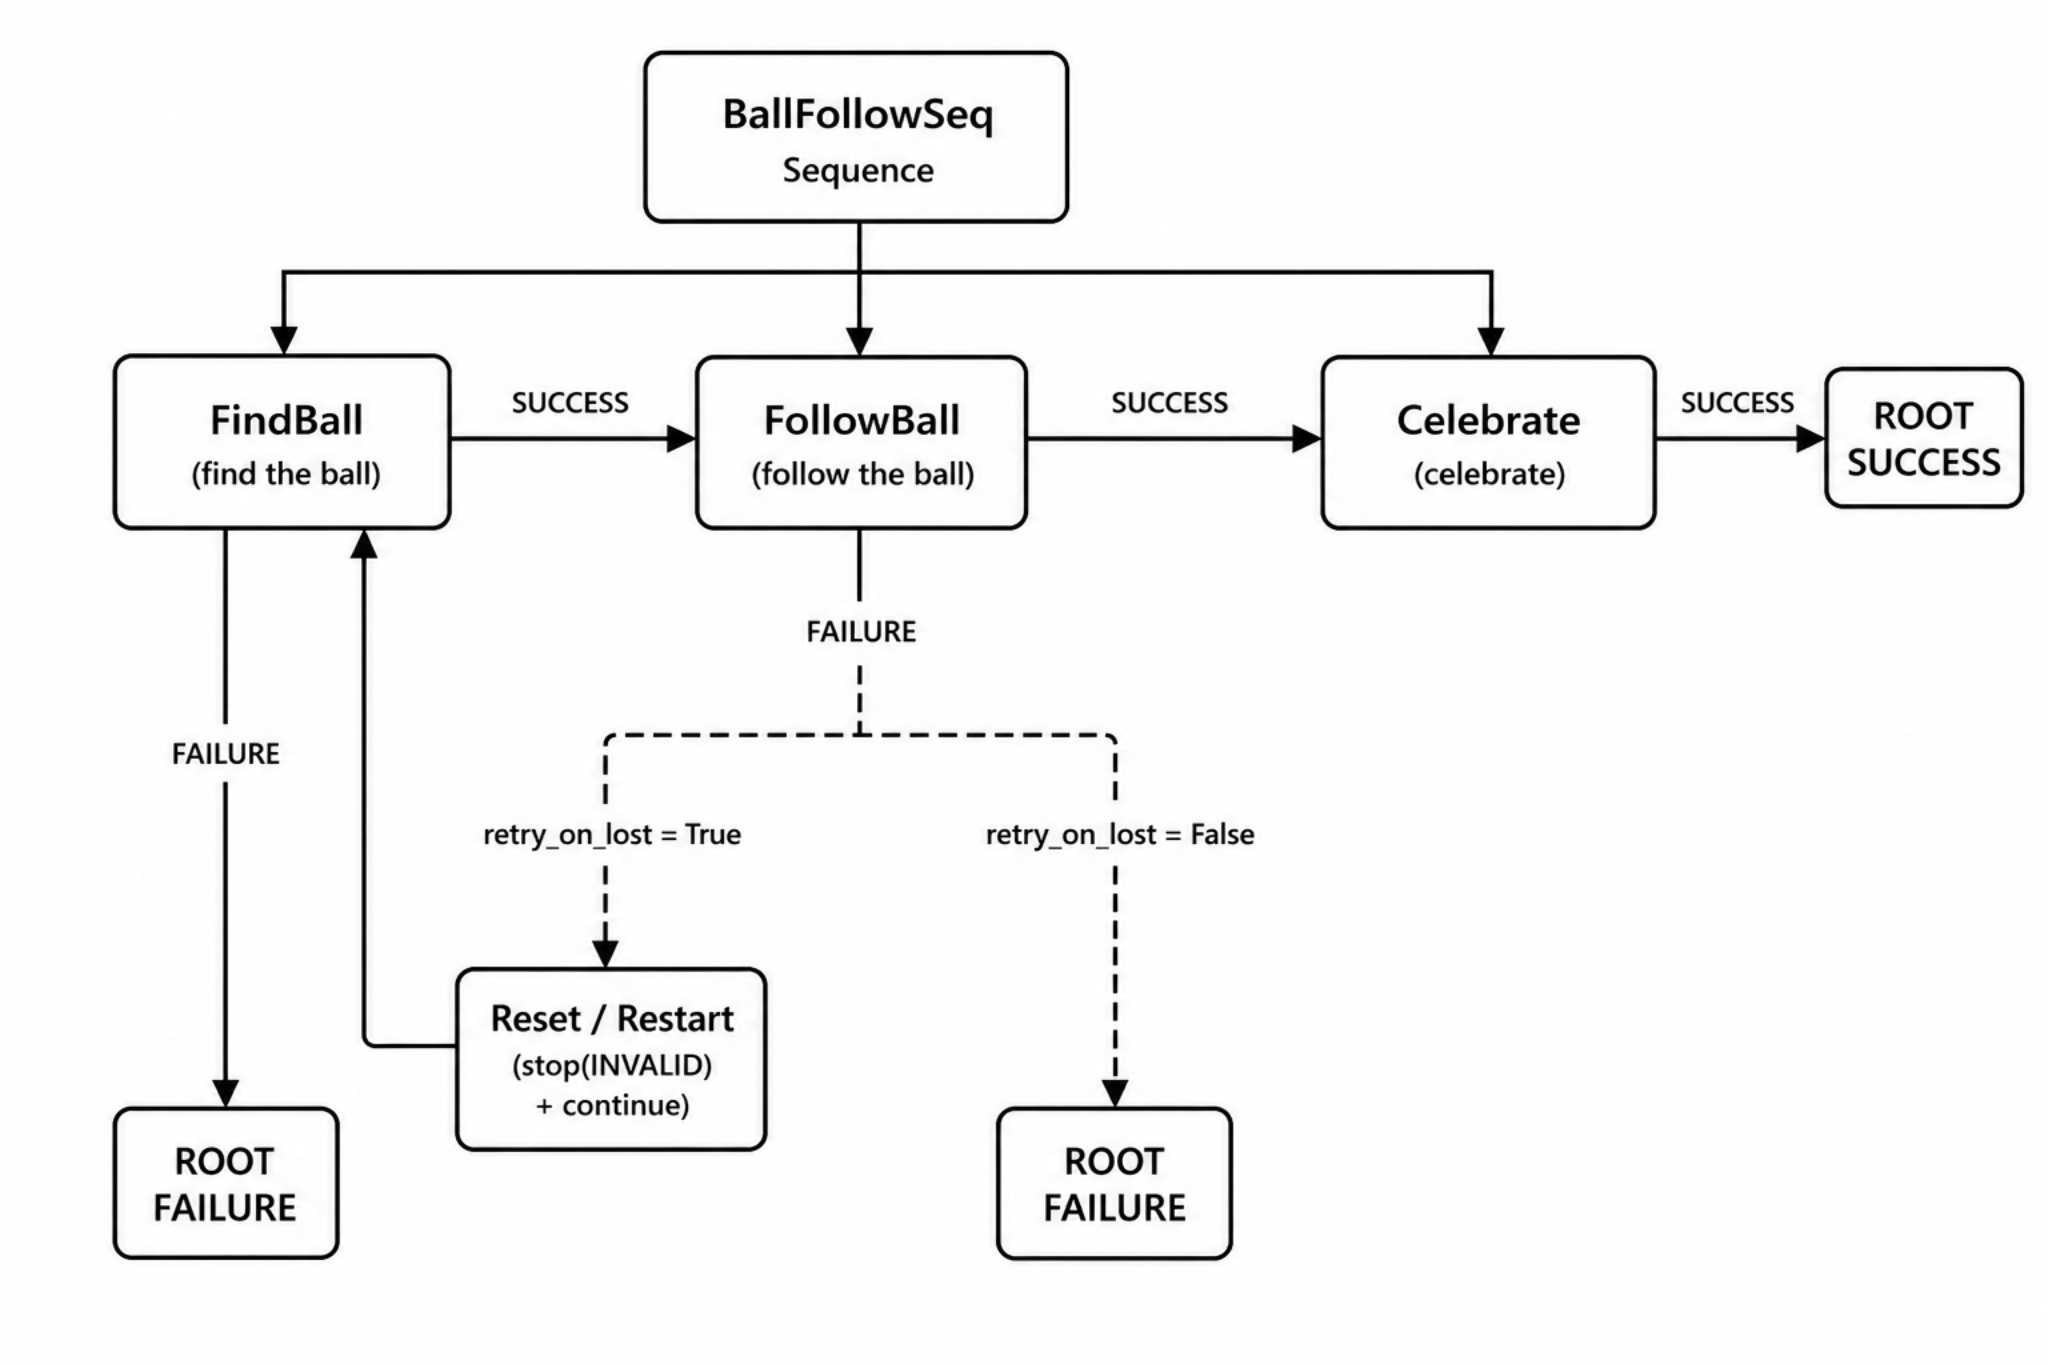
\includegraphics[width=0.7\textwidth]{obrazky/bt_diagram.png}
          \caption[Behaviorálny strom sledovania lopty]{Strom uzla \texttt{ball\_follow\_bt\_runner} (\path{ball_follow/bt_runner.py})}
          \label{fig:ball-follow-bt-diagram}
        \end{figure}
      
        Koreň stromu je sekvencia, takže po úspešnom dokončení kroku sa pokračuje ďalším bez opätovného spúšťania predchádzajúcich fáz. V prípade zlyhania sledovania môže strom skončiť chybou alebo sa celý scenár resetuje a začne znova od \textbf{FindBall}, v závislosti od parametra \texttt{retry\_on\_lost}.
      
        Behaviorálny strom tak riadi makro priebeh úlohy a samotný regulátor BallController rieši krátkodobé výpadky detekcie na nižšej úrovni.
      
        \subsubsection*{Akčný server \texttt{follow\_ball}}
      
        Metóda \texttt{\_execute\_cb} v \path{action_node.py} obsluhuje vykonávanie cieľa. Po prijatí nastaví príznaky \texttt{\_goal\_busy} a \texttt{\_active} a v pravidelnej slučke  kontroluje zrušenie a podmienky úspechu alebo zlyhania.
      
        Pre režim \textbf{FindBall} (\texttt{stop\_when\_found=True}) je kritérium že akcia skončí úspešne hneď, ako sa objaví čerstvá detekcia . V režime \textbf{FollowBall}  môže byť zapnuté aj zlyhanie pri strate objektu.
      
        Úspech pri sledovaní sa vyhodnocuje vtedy, keď je detekcia čerstvá a $\texttt{radius\_px} \geq \texttt{stop\_radius\_px}$. Časová značka sa uloží do fronty \texttt{close\_times}.
      
        \subsubsection*{Implementácia a spustenie}
      
        Systém sa spustí pomocou \path{ball_follow_standalone.launch.py}, ktorý inicializuje motor, kameru, uzol \texttt{ball\_follower} a \texttt{bt\_runner}. Alternatívne sa dá použiť aj offboard spracovanie (\texttt{offboard\_cv:=true}).
      
        \section{Runtime stack, webové rozhranie a prevádzkové služby}
      
        Webové rozhranie som do systému pridal, aby bolo jednoduché ovládať robota bez potreby 
        priamej práce s ROS~2 nástrojmi.
      
        \subsection{Webové rozhranie}
        \label{sec:web-ui-prehlad}
        \label{sec:web-ui-detail}
      
        Frontend aplikácie je implementovaný ako jednostránkové rozhranie, ktoré komunikuje s ROS~2 prostredím prostredníctvom knižnice \emph{roslibjs}~\cite{roslibjs_github} nad serverom \emph{rosbridge\_suite}~\cite{rosbridge_suite_github}. 
      
        Rozhranie poskytuje informáciu o stave pripojenia, živý obraz z kamery, tlačidlá pre pohyb robota, tlačidlá pre prepínanie režimov a parametrov regulácie a tlačítko na vzdialené vypnutie.
      
        \begin{figure}[H]
            \centering
            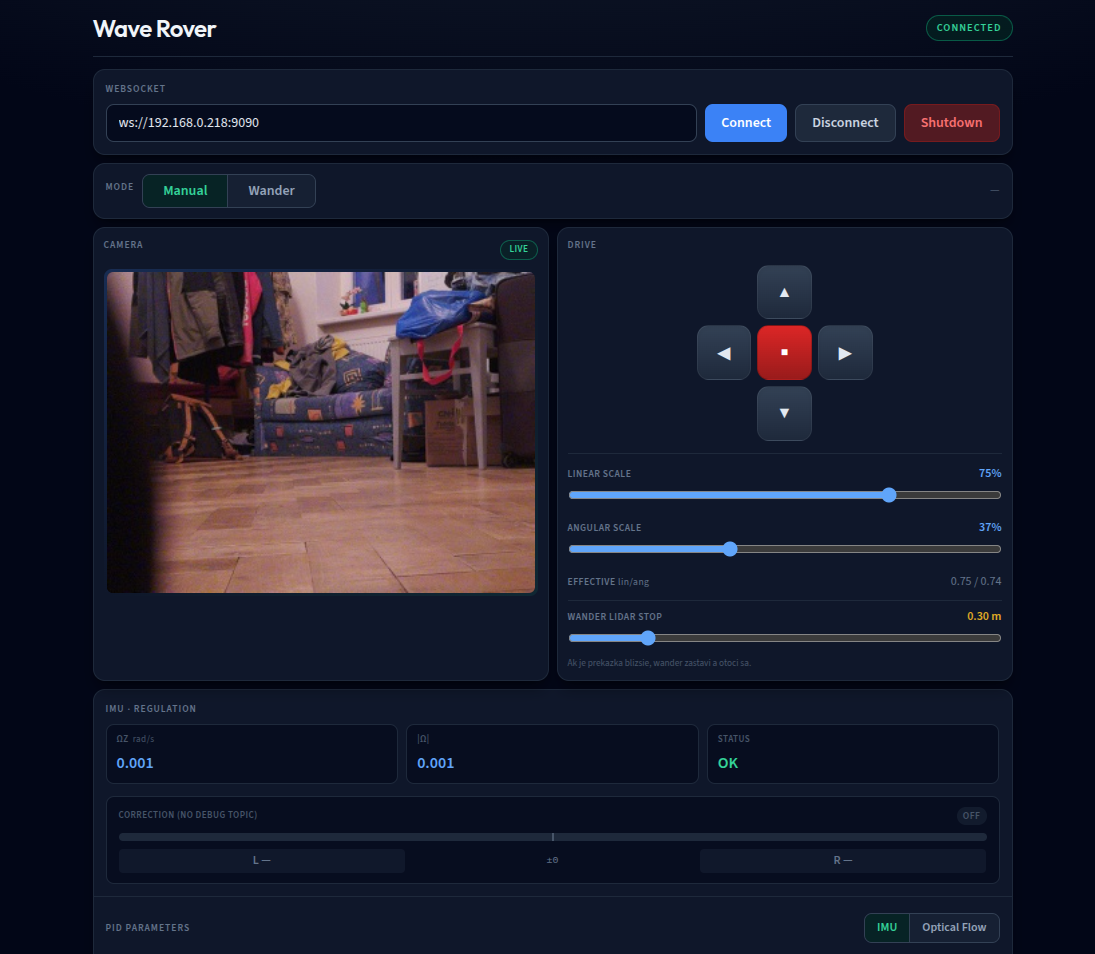
\includegraphics[width=0.75\textwidth]{obrazky/webui.png}
            \caption[Webové rozhranie robota]{Užívateľské rozhranie dostupné v prehliadači}
            \label{fig:web_ui_desktop}
        \end{figure}
      
        \subsection{Komunikačná vrstva.}
      
        Po nadviazaní WebSocket spojenia sa v klientovi vytvorí publisher na tému \rostopic{/teleop_cmd_vel}. Pohybové príkazy sa odosielajú opakovane s frekvenciou 30~Hz.
      
        Živý obraz z kamery v paneli rozhrania je riešený podľa časti~\ref{sec:web-camera-webrtc}.
      
        \subsection{Ovládanie pohybu.}
      
        Na zadávanie pohybu slúži smerový ovládač typu D-pad. Každé tlačidlo obsahuje definovanú lineárnu a uhlovú zložku pohybu. Na mobilných zariadeniach sú použité dotykové udalosti \texttt{touchstart} a \texttt{touchend}.
      
      
        \subsection{Runtime stack, prepínanie \texorpdfstring{manuál / wander}{manuál -- wander} a graf uzlov}
        \label{sec:mode_switch}
      
        Na plynulé prepínanie medzi manuálnym ovládaním a autonómnym režimom  som navrhol samostatný integračný uzol \texttt{robot\_mode\_switch}, ktorý zabezpečuje zmenu režimu za behu systému. Využíva klienta \texttt{AsyncParameterClient}, čím mení parametre iných bežiacich uzlov bez potreby ich reštartu.
        \begin{verbatim}
        self._motor = _RemoteParamClient(self, "/motor_hat_node")
        self._wander = _RemoteParamClient(self, "/lidar_wander_node")
      
        fut = self._motor.set_parameters([
            Parameter("control_mode",
                      Parameter.Type.STRING,
                      "manual")
        ])
        \end{verbatim}
      
      V ROS~2 sa dynamická rekonfigurácia rieši cez parametre uzlov. Uzol \texttt{robot\_mode\_switch} počas behu mení parametre ostatných uzlov pomocou \texttt{AsyncParameterClient}.

  Ďalšie nastavenia je možné meniť cez argumenty launch súborov a YAML konfigurácie (napr.\ voľba portu IMU, zapnutie offboard spracovania alebo výber korekcie jazdy), pričom prehľad hlavných uzlov a prepínačov je uvedený v tab.~\ref{tab:uzly-prehlad}.
      
        \subsection{Graf uzlov a dátových tokov.}
      
        Na obr.~\ref{fig:runtime-rqt-graph} je graf uzlov pri spustení \texttt{runtime\_stack.launch.py}. Je z neho vidiť prepojenie motorového uzla, uzla blúdenia, prepínača režimov, senzorických driverov a webového rozhrania.
      
        \begin{figure}[H]
            \centering
            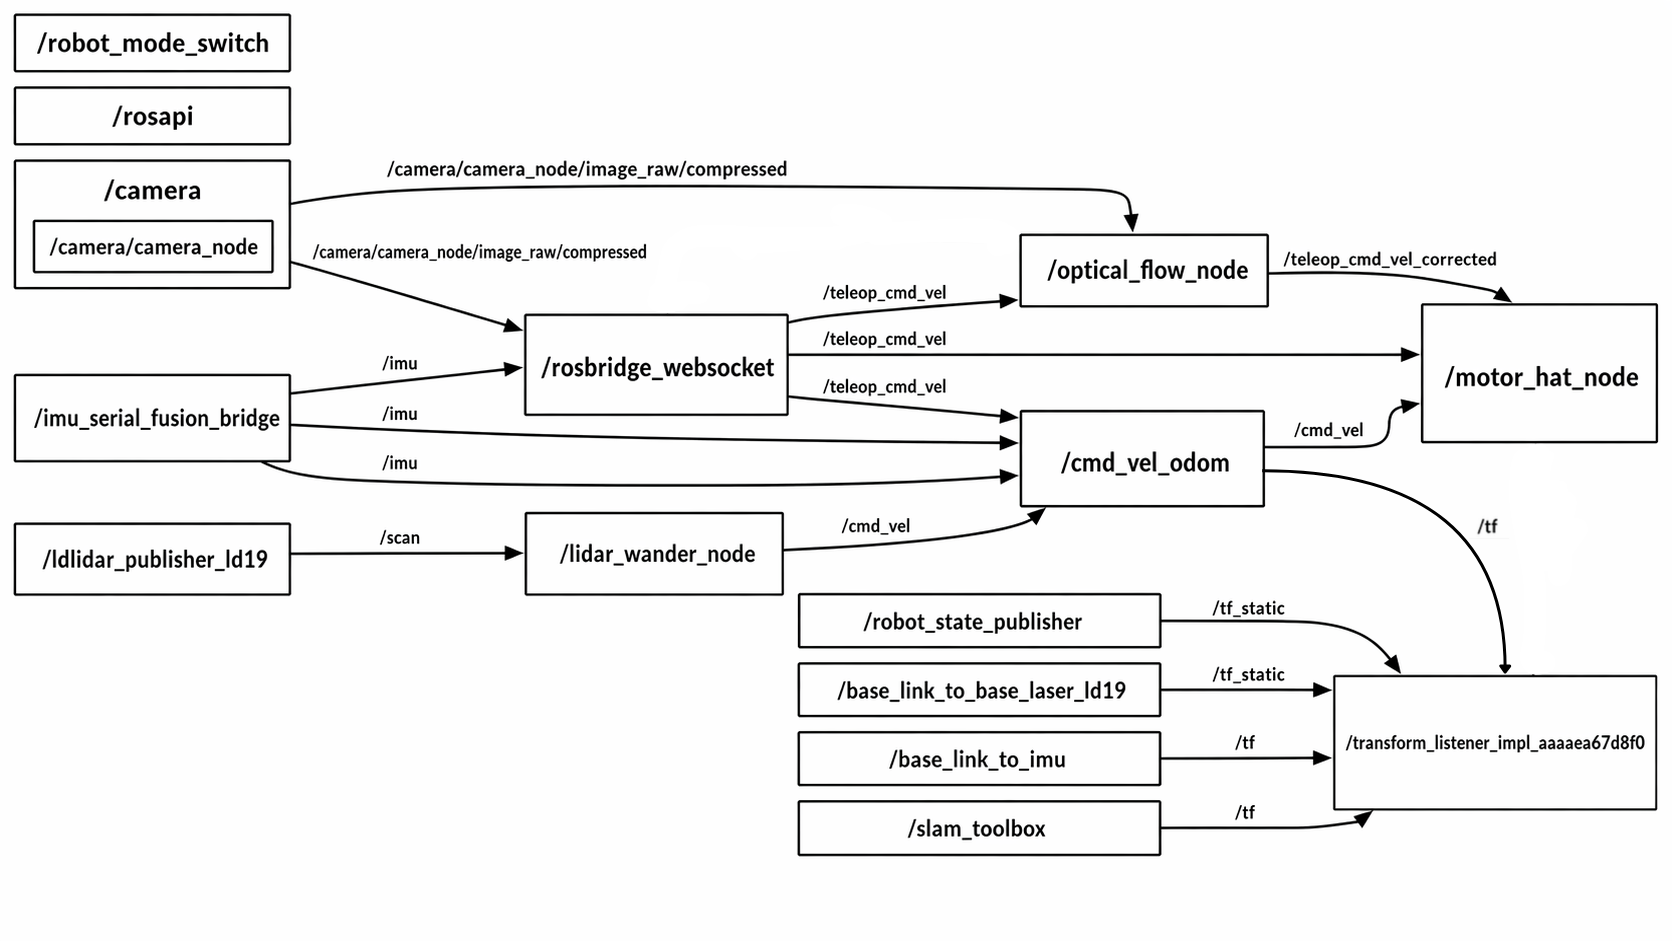
\includegraphics[width=0.98\linewidth]{obrazky/runtime_rqt.png}
            \caption[Graf uzlov pri runtime stacku]{Prepojenie hlavných uzlov, tém a služieb pri spustenej fyzickej platforme}
            \label{fig:runtime-rqt-graph}
        \end{figure}
      
      
        \subsection{Vzdialené vypnutie Raspberry Pi a tlačidlo Shutdown v používateľskom rozhraní}
  \label{sec:remote-shutdown}

  Pri používaní robota sa ukázalo ako praktické mať možnosť systém vypnúť na diaľku bez potreby pripájať klávesnicu alebo monitor.

  Túto funkcionalitu som implementoval v uzle \texttt{robot\_mode\_switch}, ktorý poskytuje službu \rostopic{/waverover/shutdown}. Po prijatí požiadavky uzol najprv odošle potvrdenie a následne vykoná príkaz \texttt{sudo systemctl poweroff}.

  \subsection{Integrita súborového systému pri výpadku napájania}
  \label{sec:fs-ro-fit}

  Pri mobilnej platforme som musel počítať aj s možnosťou náhleho odpojenia napájania. Z tohto dôvodu uprednostňujem korektné vypnutie systému cez službu \texttt{/waverover/shutdown}, ktoré znižuje riziko poškodenia dát.

  Napriek tomu sa takýmto situáciám nedá úplne vyhnúť, preto je dôležité aj vhodné nastavenie operačného systému. Jednou z možností je použitie read-only systémového oddielu, pri ktorom sa počas bežnej prevádzky nezapisuje na disk, čím sa zníži riziko poškodenia pri výpadku.

  Ak treba zapisovať dáta, dá sa využiť overlay vrstva, napríklad v RAM. Riešenie sa potom navonok správa štandardne, ale zmeny sa neukladajú priamo do úložiska.

  Ako doplnkové opatrenie sa dajú použiť aj odolnejšie pamäťové médiá~\cite{kingston_industrial_sd}, napríklad high-endurance alebo industrial microSD karty navrhnuté na časté prepisovanie dát a dlhodobú prevádzku. Oproti bežným kartám výrobcovia deklarujú vyššiu odolnosť voči zápisovým cyklom a vhodnosť pre dlhodobú prevádzku v náročnejších podmienkach. V tomto projekte sa mi však osvedčila aj bežná SD karta.
      
        \section{Overenie implementácie a prehľad uzlov}
        \label{sec:navrh-uzlov}
      
        Po návrhu a implementácii jednotlivých častí systému bolo potrebné overiť, ako sa správajú pri reálnom použití. V tejto kapitole preto opisujem testovanie robota, jeho jednotlivých režimov a vzájomnej spolupráce uzlov v ROS~2.
      
        \subsection*{Metodika testovania}
      
        Overenie systému prebiehalo praktickými jazdnými testami v domácom prostredí. Robot bol skúšaný na rôznych povrchoch a pri rôznych svetelných podmienkach. Cieľom bolo hlavne overiť, či jednotlivé režimy fungujú spoľahlivo v bežných podmienkach.
      
        Počas testovania som správanie systému sledoval pomocou nástrojov \texttt{rqt\_graph}, \texttt{rqt\_image\_view}, \texttt{rqt\_plot} a ROS~2 CLI. Pomocou \texttt{rqt\_graph} som kontroloval prepojenie uzlov a tém, \texttt{rqt\_image\_view} slúžil na sledovanie obrazových výstupov a debug streamov a \texttt{rqt\_plot} pomáhal analyzovať priebeh veličín pri korekcii smeru.
      
        \subsubsection{Ladenie IMU korekcie a PID v motorovom uzle}
      
        Ladenie IMU korekcie prebiehalo iteratívne. Najprv som overil, či sa korekcia správne aktivuje, a potom som postupne dolaďoval jednotlivé parametre. Pri rovnej jazde som riešil najmä filtráciu a mŕtvu zónu. Ak robot kmital okolo nuly, mierne som zvýšil \texttt{imu\_deadband} alebo znížil \texttt{imu\_yaw\_lowpass\_alpha}, čím sa odozva vyhladila.
      
        Parametre PID regulátora som dolaďoval postupne odhadom podľa pozorovania správania robota pri jazde.
      
        \subsubsection{Testovanie a ladenie optického toku}
      
        Optický tok som tiež ladil podľa správania robota a vizuálnej spätnej väzby. Ukázalo sa, že funguje spoľahlivo len pri dostatočnej textúre a osvetlení. Na jednofarebnom pozadí alebo pri slabom svetle bol počet sledovaných bodov nízky a odhad pohybu bol nespolahlivý.
      
        Parametre \texttt{correction\_gain} a \texttt{max\_correction} určovali silu korekcie, ktorých hodnotu som tiež ladil hlavne od sledovania jazdy, aby neboli zásahy malé ani príliš trhané.
      
        \subsubsection{Testovanie sledovania objektu}
      
        Sledovanie objektu bolo založené na HSV segmentácii a výbere kontúry podľa tvarových vlastností. Najprv som nastavoval prahy offline podľa debug obrazu, potom som testoval správanie počas jazdy.
      
        Intervaly HSV som upravoval tak, aby maska pokrývala loptu, ale nezachytávala okolie. Najcitlivejšie boli parametre $V_{\min}$ a $S_{\min}$, ktoré sa museli meniť podľa osvetlenia. Konkrétne v mojej zatienenej izbe sa maska často rozpadala, takže bolo potrebné nájsť kompromis medzi presnosťou a flexibilitou.
      
        Morfologické operácie som ladil podľa šumu masky. Tvarové parametre ako kruhovitosť, solidita a vyplnenie som najprv nastavil prísnejšie, aby som eliminoval falošné detekcie, a potom mierne uvoľňoval, aby systém zvládal aj čiastočne zakrytý objekt. Na záver som doladil \texttt{min\_confidence}, ktorý pomáhal vybrať najlepšiu kontúru.
      
        \subsubsection{Limity platformy}
      
        Jedným z hlavných obmedzení platformy je absencia enkodérov na kolesách. Odometria sa preto odhadovala bez priamej spätnej väzby z kolies. Poloha $x,y$ vznikala spracovaním odosielaného \texttt{cmd\_vel} a orientácia \texttt{yaw} bola preberaná z IMU. Systém tak predpokladal ideálne vykonanie príkazov, čo však neplatilo vždy a bolo to viditeľné pri pohybe modelu v RVize aj fyzického robota.
      
        Ďalším zdrojom nepresnosti je gyroskop. Vo wander režime sa tento problém prejavoval napríklad pri otočkách, kde uhol odhadoval integráciou uhlovej rýchlosti $\omega_z$, ktorá je citlivá na chyby merania. V dôsledku toho sa robot niekedy otočil o trochu viac alebo menej, než bolo zamýšľané; pri dlhšom behu sa drift môže prejaviť aj pomalou zmenou odhadu natočenia aj v pokoji.
      
        \subsection{Výsledky testov}
      
        Testovanie ukázalo, že systém je schopný spoľahlivo fungovať vo všetkých hlavných režimoch. Prepínanie medzi manuálnym a autonómnym riadením prebiehalo plynulo, bez potreby reštartu uzlov, čo potvrdzuje správny návrh komunikačnej vrstvy a mechanizmu prepínania režimov.
      
        Režim wander dokázal reagovať na prekážky a pokračovať v pohybe bez zásahu používateľa. V meraniach odchýlky jazdy vychádza najlepšie optical flow, no jeho kvalita je citlivá na osvetlenie a textúru prostredia. Z pohľadu prevádzkovej stability musím ako lepšiu variantu vyhodnotiť IMU korekciu, ktorá fungovala použiteľne aj pri rôznych svetelných podmienkach a rozmanitosti prostredia.
      
        Sledovanie lopty fungovalo po doladení HSV prahov a geometrických podmienok pomerne stabilne, pričom problémy sa opäť objavovali pri zmenách svetelných podmienok alebo v tieni. To ale patrí medzi bežné obmedzenia jednoduchých farebných segmentačných metód.
      
        \subsection{Diskusia výsledkov a ďalší vývoj}
      
        Získané výsledky potvrdili, že ROS~2 architektúra je vhodná pre modulárny návrh robotického systému. Jednotlivé komponenty bolo možné samostatne testovať, upravovať a kombinovať, čo uľahčilo vývoj aj ladenie.
      
        Zároveň sa ukázalo, že presnosť celého systému je ovplyvnená hardvérovými obmedzeniami. Absencia enkodérov spôsobuje nepresnú odometriu, drift IMU ovplyvňuje stabilitu smeru a kamera je citlivá na zmeny osvetlenia. Tieto faktory sa navzájom kombinujú a priamo ovplyvňujú kvalitu jazdy aj detekcie objektov.
      
        Získané poznatky naznačujú, že ďalší vývoj by sa mohol zamerať na doplnenie enkodérov, ktoré by poskytli presnejšiu spätnú väzbu o pohybe robota.  Zlepšenie by v tomto ohľade priniesla aj pokročilejšia fúzia senzorov.

  V oblasti kamery a spracovania obrazu by som do budúcna nahradil jednoduchú farebnú segmentáciu modernejšími prístupmi založenými na strojovom učení.
      
        \subsection{Uzly a ich funkcie v systéme}
      
        Pre lepší prehľad slúži tabuľka~\ref{tab:uzly-prehlad}. Ide o zhrnutie uzlov, ktoré priamo zodpovedajú funkcionalite opísanej v tejto kapitole.
      
        % longtable: rozdelenie na viac strán (tabularx v table[H] spôsobovalo prázdnu stranu a orezanie cez pätičku)
        \begin{longtable}{@{}>{\raggedright\arraybackslash}p{0.36\textwidth}>{\raggedright\arraybackslash}p{0.56\textwidth}@{}}
          \caption{Hlavné ROS~2 uzly používané v práci}
          \label{tab:uzly-prehlad} \\
          \toprule
          Uzol (ROS meno) & Účel \\
          \midrule
          \endfirsthead
          \caption[]{Hlavné ROS~2 uzly používané v práci (pokračovanie)} \\
          \toprule
          Uzol (ROS meno) & Účel \\
          \midrule
          \endhead
          \midrule
          \multicolumn{2}{r}{\small\itshape Pokračuje na nasledujúcej strane} \\
          \endfoot
          \bottomrule
          \endlastfoot
          LD19 (\texttt{ldlidar\_ros2}) &
            Ovládač LiDARu, publikuje sken na \rostopic{/scan}. \\
          \midrule
          \texttt{imu\_serial\_fusion\_bridge} &
            Most z Arduino IMU do ROS~2, publikuje \rostopic{/imu}. \\
          \midrule
          \texttt{camera\_node} (\texttt{camera\_ros}) &
            Kamerový vstup, publikuje obraz a \texttt{camera\_info}. \\
          \midrule
          \texttt{webrtc\_camera} (\path{webrtc_camera_node.py}) &
            Prenáša obraz do webového rozhrania cez WebRTC. \\
          \midrule
          \texttt{motor\_hat\_node} (\texttt{waverover\_motor}) &
            Riadi motory robota podľa príkazov rýchlosti. \\
          \midrule
          \texttt{lidar\_wander\_node} (\path{lidar_wander.py}) &
            Jednoduché autonómne blúdenie podľa LiDARu, výstup na \rostopic{/cmd_vel}. \\
          \midrule
          \texttt{robot\_mode\_switch} (\path{robot_mode_switch.py}) &
            Prepína režimy robota cez ROS~2 služby (manual/wander/nav). \\
          \midrule
          \texttt{teleop\_twist\_keyboard} &
            Klávesnicové manuálne ovládanie robota. \\
          \midrule
          \texttt{optical\_flow\_node} (\texttt{optical\_flow}) &
            Vizuálna korekcia smeru jazdy podľa optického toku. \\
          \midrule
          \texttt{cmd\_vel\_odom} (\path{cmd_vel_odom.py}) &
            Odhad odometrie z príkazov rýchlosti, publikuje \rostopic{/odom} a TF. \\
          \midrule
          \texttt{base\_link\_to\_imu} (\texttt{static\_transform\_publisher}) &
            Statická transformácia medzi telom robota a IMU. \\
          \midrule
          \texttt{slam\_toolbox} (\texttt{async\_slam\_toolbox\_node}) &
            Tvorba 2D mapy a lokalizácia v mape (SLAM). \\
          \midrule
          \texttt{ekf\_filter\_node} (\texttt{ekf\_node}) &
            Fúzia senzorových dát cez EKF (\texttt{robot\_localization}). \\
          \midrule
          \texttt{odom\_to\_base\_link} (\texttt{static\_transform\_publisher}) &
            Núdzová statická transformácia \texttt{odom}$\rightarrow$\texttt{base\_link}. \\
          \midrule
          \texttt{robot\_state\_publisher} &
            Publikuje TF strom robota z URDF/Xacro modelu. \\
          \midrule
          \texttt{rviz2} &
            Vizualizácia dát, mapy a TF počas testovania. \\
          \midrule
          \texttt{rosbridge\_websocket}, \texttt{rosapi} &
            Prepojenie webového rozhrania s ROS~2 cez WebSocket API. \\
          \midrule
          \texttt{simple\_nav\_node} (\path{simple_nav_node.py}) &
            Jednoduchá bodová navigácia na zadaný cieľ. \\
          \midrule
          \texttt{ball\_follower} (\path{action_node.py}) &
            Deteguje a sleduje farebný objekt, riadi robot pri sledovaní lopty. \\
          \midrule
          \texttt{ball\_follow\_bt\_runner} (\path{bt_runner.py}) &
            Vyššia logika úlohy sledovania lopty pomocou behaviorálneho stromu. \\
        \end{longtable}
      
  \chapter{Záver}

  Cieľom práce bolo navrhnúť a implementovať riadiaci softvér pre mobilnú platformu Wave Rover s využitím ROS~2 na Raspberry Pi. Počas práce sa mi podarilo vytvoriť funkčný systém, ktorý prepája jednotlivé hardvérové aj softvérové časti do jedného celku a umožňuje jeho ďalšie rozširovanie. Na základe implementácie a praktického testovania možno konštatovať, že stanovené ciele práce sa podarilo splniť.

  Výsledkom je vlastný balík \texttt{waverover}, v ktorom som postupne implementoval riadenie pohonu, spracovanie dát zo senzorov, kamerový subsystém aj rôzne režimy riadenia. Systém som testoval na fyzickom robote aj v simulácii, čo mi umožnilo lepšie pochopiť rozdiely medzi ideálnym modelom a reálnym správaním platformy.

  Počas implementácie a testovania som si všimol, že najväčšou výzvou nebolo samotné naprogramovanie jednotlivých častí, ale ich vzájomné prepojenie a ladenie. Mnohé problémy sa prejavili až pri jazde robota, napríklad nestabilita smeru alebo nepresnosti v odometrii, čo viedlo k postupným úpravám parametrov a celkového návrhu.

  Praktické testovanie zároveň ukázalo aj limity použitej platformy. Absencia enkodérov sa prejavuje v nepresnej odometrii, IMU bez magnetometra vykazuje drift a optický tok je citlivý na osvetlenie a štruktúru prostredia. Tieto obmedzenia sú však typické pre jednoduchšie riešenia a bolo zaujímavé sledovať, ako sa navzájom ovplyvňujú.

  Aj napriek objaveným nedostatkom je s touto platformou možné vytvoriť funkčný a modulárny robotický systém, ktorý je vhodný na experimentovanie a overovanie rôznych prístupov v prostredí ROS~2. Práca mi zároveň poskytla praktickú skúsenosť s návrhom a ladením robotického systému v reálnych podmienkach.

  Do budúcna by sa projekt dal rozšíriť napríklad o enkodéry pre presnejšiu odometriu, lepšiu fúziu senzorových dát alebo pokročilejšie metódy spracovania obrazu, napríklad detekčné modely YOLO\footnote{\url{https://arxiv.org/abs/1506.02640}}. Navrhnutý systém tak predstavuje dobrý základ pre ďalšie experimentovanie a rozvoj v oblasti mobilnej robotiky.
      